\documentclass[a4paper, 11pt, twoside]{book}

% including package
\usepackage{times}
\usepackage{makeidx}
\usepackage{fancyhdr}
\usepackage{amsmath, amsthm, mathtools}
\usepackage[dvipdfmx]{graphicx}
\usepackage[top=25truemm,bottom=25truemm,left=22.5truemm,right=22.5truemm]{geometry}
\usepackage[nottoc, notlot, notlof]{tocbibind}
\usepackage{CJKutf8}
\usepackage[titletoc]{appendix}
\usepackage{float}
\usepackage{subcaption}
\usepackage[dvipdfmx, colorlinks=true, 
			linkcolor=blue, citecolor=red,
			bookmarks=true, bookmarkstype=toc]{hyperref}
\usepackage{url}
\usepackage[font=small]{caption}
\usepackage{setspace}
\setstretch{1.28}
%\setlength{\textheight}{41\baselineskip}
%\addtolength{\textheight}{\topskip}

\pagestyle{fancy}
%\fancyhf{}
%\fancyhead[EL]{\slshape \nouppercase \leftmark}
%\fancyhead[OR]{\slshape \nouppercase \rightmark}
%\fancyhead[ER,OL]{\thepage}
\fancyhead{}
\fancyhead[RO, RE]{\slshape \nouppercase \rightmark}
\fancyhead[LE, LO]{\slshape \nouppercase \leftmark}
\cfoot{\thepage}

\renewcommand{\bibname}{References}

\makeatletter
\def\@biblabel#1{(#1)}
\def\@cite#1{\textsuperscript{(#1)}}
\makeatother

\begin{document}

 \frontmatter
  \begin{titlepage}
 
 \begin{figure}[htbp]
  
\includegraphics[clip, width=3.3cm]{./others/fig/kyushulogo.pdf}
 \end{figure}
 
 \null
 \vfill
 
 \begin{center}
  \Large{\sc Master Thesis}

  \vspace{10truemm}

  \LARGE{\bf Radiation study on the Superconducting Solenoid Magnet for $\mu^- \rightarrow e^-$ Conversion Experiment}\\
  
  \Large{\begin{CJK}{UTF8}{min}$BOBLu!'%_%e!<%*%sEE;RE>49C5:w<B83$K$h$kJ|<M@~4D6-2<$K$*$1$kD6EAF3%=%l%N%$%I<'@P$K4X$9$k8&5f(B\end{CJK}}\\

  \vspace{10truemm}
  
  \Large{Ye, YANG}\\
  \it Radiation Physics and Measurement,  \\
  \it Department of Applied Quantum Physics and Nulcear Engineering, \\
  \it Kyushu University  \\
 \end{center}
 \vfill
 \begin{flushright}
  \begin{tabular}{rl}
   Supervisor:         &  \it Kenji, ISHIBASHI (Kyushu University)  \\
   					   &  \it Nobuhiro, SHIGYO (Kyushu University)  \\
					   &  \it Toru, OGITSU (KEK)  \\
				 	   &  \it Mokoto, YOSHIDA (KEK)  \\
   Registration date:  &  \\
   Submission date:    &  \\
  \end{tabular}
 \end{flushright}
\end{titlepage}

\clearpage
\thispagestyle{empty}
%\cleardoublepage

%\chapter*{\centering Abstract}



\tableofcontents

\listoffigures

\listoftables


 \mainmatter
  \chapter{Introduction}
~~~~~~Although the Higgs boson has been found in 2012 by CMS and ATLAS collaboration~\cite{higgs}, there are no clues of new physics in last running with 3.5 TeV per beam.
the Standard Model still remains many unsolved problems such as neutrino oscillation, the lack of dark matter candidate, fine-tuning and matter anti-matter asymmetry.
On the other hand, it is known that the quarks and neutrinos are mixing as the Cabibbo-Kobayashi-Maskawa (CKM) matrix and Pontecorvo-Maki-Nakagawa-Sakata (PMNS) matrix, respectively~\cite{mark}.
However, as the same family with neutrino, it is strange that charged lepton flavor violation (cFLV) is still not founded.
As the prediction of lower branching ratio from the physics beyond the Standard model (BSM), new physics is possible to be probed through the cLFV.

Coherent muon to electron transition (COMET) experiment is planning to seek the cLFV channel of $\mu^- N \rightarrow e^- N$ from 2017.
To achieve the better sensitivity, the most intense muon beamline in J-PARC is under designing and construction.

\section{Charged lepton flavor violation}
~~~~~~In Standard Model, the neutrino oscillation is constricted and massless, in addition, the lepton number is totally conserved when they decay, like
\begin{eqnarray*}
 & \mu^- & \rightarrow  e^-  +  v_\mu  +  \bar v_e  \\
 L_\mu: & 1 & \quad\; 0 \qquad 1 \qquad\! 0 \\
 L_e: & 0 &   \quad\; 1 \qquad 0 \quad -1 
\end{eqnarray*}
where the electron lepton number $L_e$ and muon lepton number $L_\mu$ on left side is conserved on right side.
This decay is the ordinary muon decay and also called Michel decay.
However this is not the only decay for muon, all kinds of muon decay is listed in table~\ref{mudecay}~\cite{pdg}.

Unlike to the michel decay, decay mode of charged lepton like $\mu^- \rightarrow e^- \gamma$ has very tiny probability of decay, observely, its electron and muon lepton number are not conserved on two sides.
The branching ratio predicted by standard model is less than 10$^{-54}$, which the details are described in Appendix.
Otherwise, the physics beyond the standard model such as SUSY-Seasaw, SUSY-GUT etc. predicts the branching ratio higher than 10$^{-15}$, which is possible to be obversed.
The reaction like this is called charged lepton flavor violation.
\begin{table}[H]
 \centering
 \begin{tabular}{cccc} \hline \hline
  Decay modes & Fraction ($\Gamma_i/\Gamma$) & Confidence level & Reference \\ \hline
  $\mu^- \rightarrow e^- \bar\nu_e \nu_\mu$ & $\approx$100 \% & & \\
  $\mu^- \rightarrow e^- \bar\nu_e \nu_\mu \gamma$ & 1.4$_{\pm 0.4}$ \% &  & \cite{critt} \\
  $\mu^- \rightarrow e^- \bar\nu_e \nu_\mu e^+ e^-$ & 3.4$_{\pm 0.4}\times$10$^{-5}$ & &  \\ \hline
  Flavor violating modes & & & \\ \hline
  $\mu^- \rightarrow e^- \nu_e \bar\nu_\mu$ & \textless 1.2 \% & 90 \% & \cite{free} \\
  $\mu^- \rightarrow e^- \gamma$ & \textless 2.4$\times$10$^{-12}$ & 90 \% & \cite{bolton} \\
  $\mu^- \rightarrow e^- e^+ e^-$ & \textless 1.0$\times$10$^{-12}$ & 90 \% & \cite{bertl} \\
  $\mu^- \rightarrow e^- \gamma \gamma$ & \textless 7.2$\times$10$^{-11}$ & 90 \% & \\ \hline \hline
 \end{tabular}
 \caption{Decay modes and branching ratio of muon.}
 \label{mudecay}
\end{table}


\section{Searches for cLFV with muon}
~~~~~$\mu \rightarrow e\gamma$, $\mu \rightarrow eee$ and $\mu \rightarrow e$ conversion are three main decay modes for cFLV seeking, and each mode has its different view in $\mu \rightarrow e$ transition.
In these modes, $\mu \rightarrow e\gamma$ and $\mu \rightarrow eee$ belong to a dipole-type like interaction, however, $\mu \rightarrow e$ conversion is a four-fermion like interaction.
The effective Lagrangian which includes both dipole-type and four-fermion operators is given by~\cite{degou}.
\begin{equation}
 \mathcal{L} = \frac{1}{1+\kappa}\frac{m_\mu}{\Lambda^2}\bar{\mu}_R\sigma^{\mu\nu}e_LF_{\mu\nu} + \frac{\kappa}{1+\kappa}\frac{1}{\Lambda^2}(\bar\mu_L\gamma^\mu e_L)(\bar q_L\gamma_\mu q_L)
 \label{phtoeq}
\end{equation}
%\begin{figure}[H]
% \centering
% 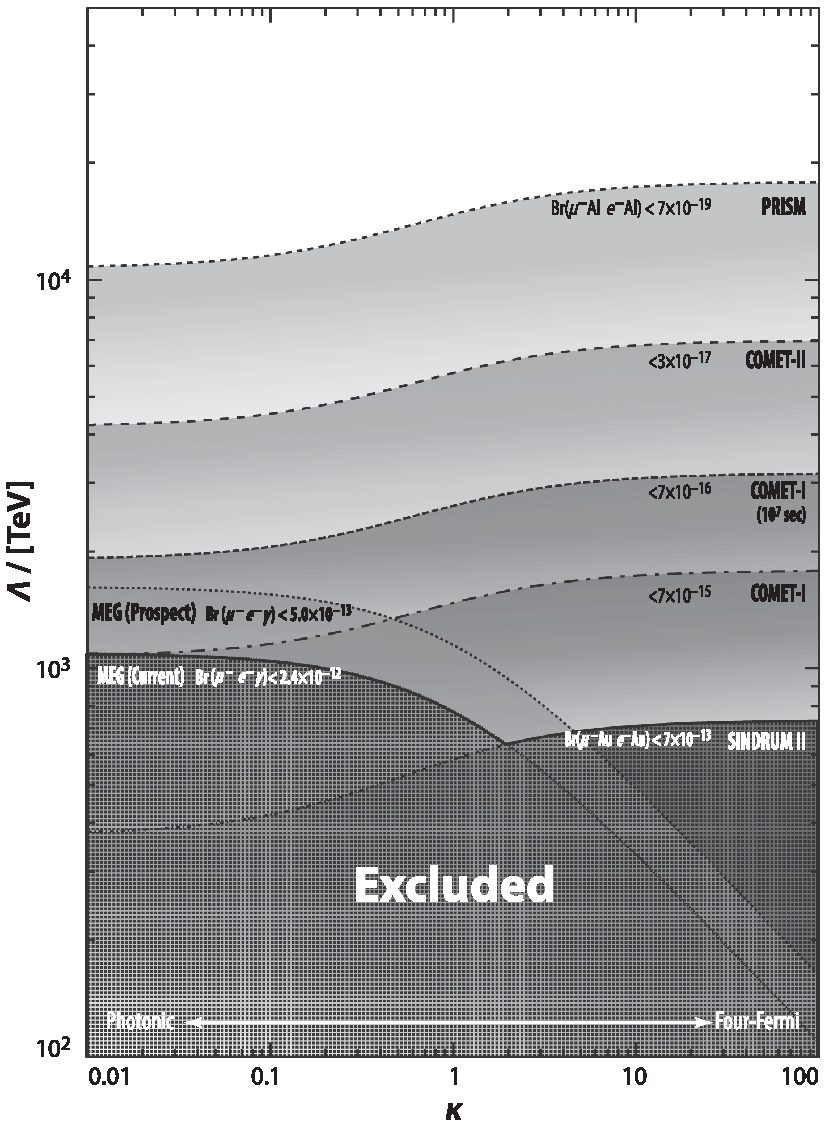
\includegraphics[scale=0.45]{chapter1/fig/photonic.pdf}
% \caption{\it Relation between dipole-like and four-fermion contribution in cLFV.}
% \label{photonic}
%\end{figure}
where $\kappa$ is a parameter which governs the relative size of dipole-type and four-fermion operators.
Parameter $\Lambda$ represents the effective mass (energy) scale of new physics.
The first and second term of this equation are meant to the dipole-like ($\kappa \ll 1$) and four-fermion interaction ($\kappa \gg 1$), which correspond to $\mu \rightarrow e\gamma$ and $\mu \rightarrow e$ conversion, respectively.
%As the result of equation~\ref{phtoeq} shown in figure~\ref{photonic}, the energy scale of new physics is possible to be explored in the TeV range, which exceeds to the range of LHC.

\subsection{$\mu \rightarrow e \gamma$}
~~~~~$\mu \rightarrow e\gamma$ is a 2-body back-to-back decay with monoenergetic $e$ and $\gamma$.
The way to search this decay is to reconstruct these back-to-back monoenergetic $e$ and $\gamma$.
The earliest $\mu \rightarrow e\gamma$ search dates back to 1947 with branching ratio of 0.1 (90\% C.L.)~\cite{1947}, and the most recent experiment for seeking this mode is the MEG experiment.

MEG experiment searches the $\mu^+ \rightarrow e^{+}\gamma$ in Paul Scherrer Institute (PSI) with 3$\times$10$^7$ $\mu^+/sec$.
The data is taken from 2009 to 2010, and MEG experiment is now under upgrading to the phase-II experiment.
As the result, MEG collaboration presents a new upper limit on the branching ratio of this decay of 5.7$\times$10$^{-13}$ (90\% C.L.) with 3.6$\times$10$^{14}$ stopped muons on target~\cite{meg}.

Unfortunately, with the branching ratio of 5.7$\times$10$^{-13}$, there is no signal of interest founded finally.
The MEG-II experiment will start data-taking from 2016 to 2019 with 180 days per year and aim to reach the branching ratio of 6$\times$10$^{-14}$~\cite{megtdr}.

\subsection{$\mu \rightarrow eee$}
~~~~~The first experiment for searching $\mu \rightarrow eee$ decay is taken in 1958 at Nevis cyclotron with the branching ratio of 3.0$\times$10$^{-5}$~\cite{lyn}.
Recent best branching ratio is 10$^{-12}$ which is measured by SINDRUM-I experiment.
A new experiment called Mu3e purposes to start from 2016 to reach a branching ratio of $\textless$ 10$^{-16}$ with the requirement of muon stop rate of about 2$\times$10$^9$ $\mu^+$/sec.
Mu3e has two phases, which phase-I and phase-II will taken in $\pi$E5 beamline and HiMB beamline of PSI respectively.

Unlike to $\mu \rightarrow e\gamma$ decay, $\mu^+ \rightarrow e^+e^+e^-$ is a 3-body decay.
The reconstruction of signal of positron and electron must be from the same vertex.
Thus, the challenges of Mu3e are the vertex, timing and momentum resolution~\cite{mu3e}.

\subsection{$\mu \rightarrow e$ conversion}
~~~~~$\mu \rightarrow e$ conversion is a different process from the other two, because the processes of $\mu \rightarrow e\gamma$ and $\mu \rightarrow eee$ are detector-limited owing to accidental background, whilst, the $\mu \rightarrow e$ conversion has no accident background but the background from beam, which depends on the beam qualities.
The past experiments for searching $\mu^- \rightarrow e^-$ conversion is listed in table~\ref{muehis}.
\begin{table}[H]
 \centering
 \begin{tabular}{cccc} \hline \hline
  Target & Upper limit & Place/Collaboration & Year \\ \hline
  Cu & $\textless$ 1.6$\times$10$^{-8}$ & SREL & 1972 \\
  $^{32}$S & $\textless$ 7$\times$10$^{-11}$ & SIN & 1982 \\
  Ti & $\textless$ 1.6$\times$10$^{-11}$ & TRIUMF & 1985 \\
  Ti & $\textless$ 4.6$\times$10$^{-12}$ & TRIUMF & 1988 \\
  Pb & $\textless$ 4.9$\times$10$^{-10}$ & TRIUMF & 1988 \\
  Ti & $\textless$ 4.3$\times$10$^{-12}$ & PSI/SINDRUM II & 1993 \\
  Pb & $\textless$ 4.6$\times$10$^{-11}$ & PSI/SINDRUM II & 1996 \\
  Ti & $\textless$ 6.1$\times$10$^{-13}$ & PSI/SINDRUM II & 1998 \\
  Au & $\textless$ 7$\times$10$^{-13}$ & PSI/SINDRUM II & 2006 \\ \hline \hline
 \end{tabular}
 \caption{History of $\mu^- \rightarrow e^-$ conversion experiments.}
 \label{muehis}
\end{table}
The most precision branching ratio is measured by SINDRUM-II experiment with gold target at PSI.
As shown in figure~\ref{sind}, there is one event found at high momentum region, but it just outside the region of interest.
\begin{figure}[H]
 \centering
 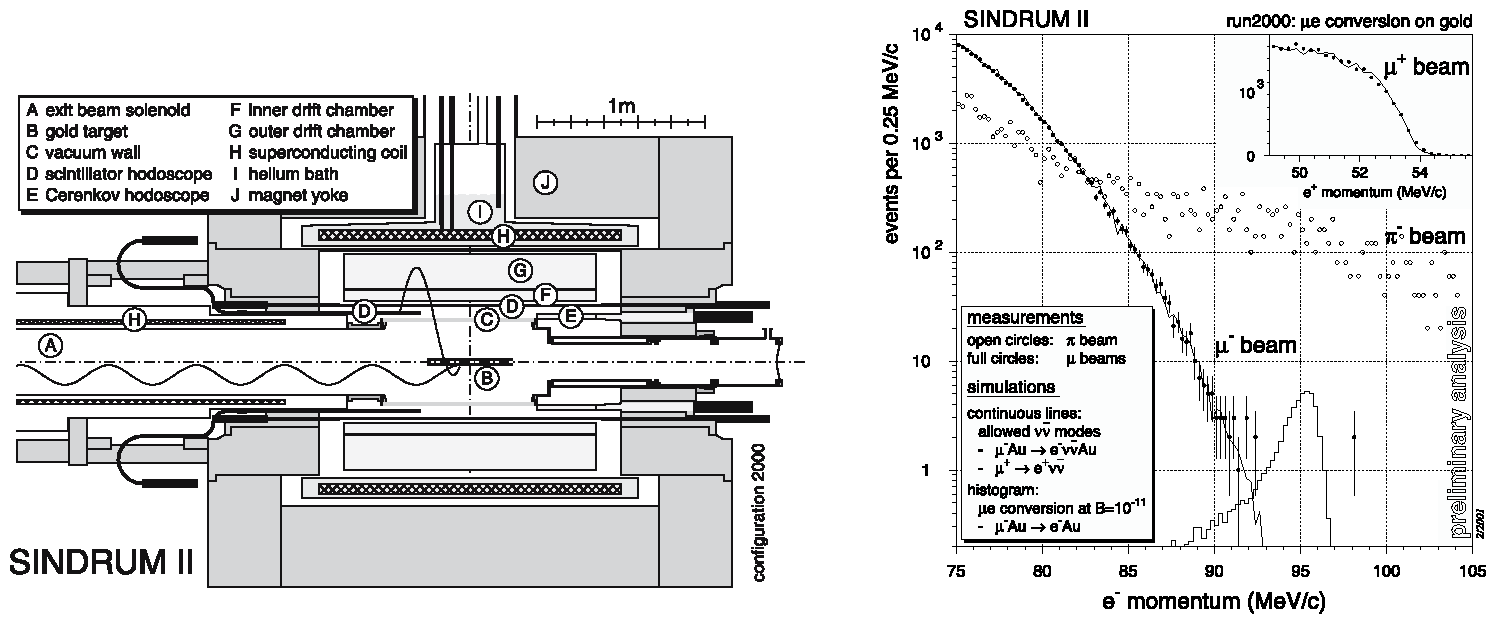
\includegraphics[scale=0.5]{chapter1/fig/sindrum.pdf}
 \caption{SINDRUM-II experiment observes a $\mu^- + Ti \rightarrow e^- + Ti$ conversion with branching ratio of 7$\times$10$^{-13}$. Two signal is founded in high energy region but it is out of the range of $\mu^- \rightarrow e^-$ signal.}
 \label{sind}
\end{figure}
COMET and Mu2e experiment are aiming to achieve the branching ratio less than 10$^{-17}$, which is 4 orders less than the previous experimental result.

\section{COMET experiment}
~~~~~~The COMET experiment is designed to search the following $\mu \rightarrow e$ conversion and be carried out at J-PARC.
\begin{equation}
 \mu^- + N(A, Z) \rightarrow e^- + N(A, Z)
\end{equation}
It has two steps for serching cLFV, which are phase-I and phase-II.
phase-I experiment is to measure the background and search for cLFV because the $\mu \rightarrow e$ conversion totally depends on the beam qualities.
phase-II experiment is to seach the $\mu \rightarrow e$ conversion with the sensitivity of 3$\times$10$^{-17}$.
As shown in figure~\ref{comet}, 8 GeV proton hits the target to produce pions, then these pions are captured by magnetic field and transported to the stopping target to generate the signal of $\mu \rightarrow e$ conversion.
The background measurement is taken at the end of 90 degree bending.

To achieve the experimental sensitivity of 3$\times$10$^{-17}$ which corresponds to the branching ratio, a total 2$\times$10$^{18}$ muons stopped in stopping target is needed.
Thus, the high intense muon source with about 10$^{11}$ $\mu^-$/sec is required for COMET experiment.
As for COMET experiment, one COMET dedicated beamline is under construction in J-PARC.
\begin{figure}[H]
 \centering
 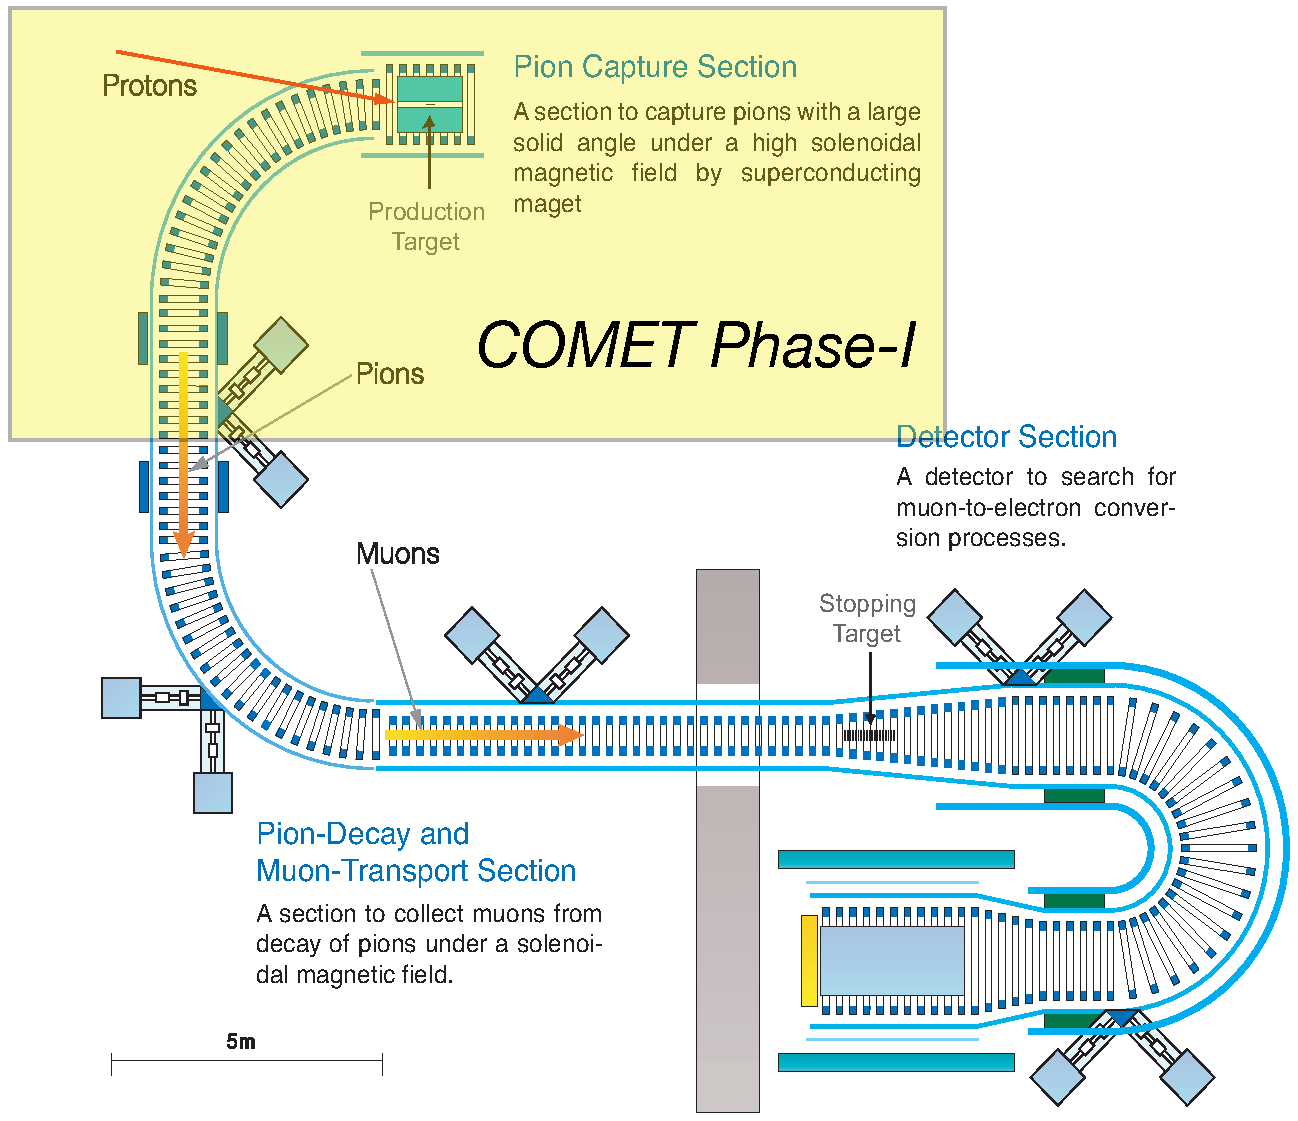
\includegraphics[scale=0.55]{chapter1/fig/comet.pdf}
 \caption{A schematic layout of COMET. 8 GeV proton from B-line hits the target and produce pion first, these pions are captured by pion capture solenoid, and decays to muons in muon transport solenoid. Then, the muon with low momentum is captured by stopping target, meanwhile, an electron with 105 MeV/c from $\mu \rightarrow e$ conversion will be transported to E-cal to take a measurement by detector solenoid.}
\label{comet}
\end{figure}

\subsection{Proton beamline}
~~~~~~To obtain the more precision branching ratio of $\mu \rightarrow e$ conversion, more stopped muon is required.
Stopped muon can be gained from two ways, increasing the operating time and increasing the muon beam intensity.
Since the most intense muon beamline over the world is located in PSI, and it only provides the muon with 4$\times$10$^8$, a new high intense muon beamline is necessary for future particle physics.
Table~\ref{protonbeam} lists the current and future muon beamline, apparently, COMET muon beamline will be the most intense muon beamline over the world in future.
\begin{table}[H]
 \centering
 \begin{tabular}{llll} \hline \hline
 Lab/Beamline & Energy and power & Present $\mu$ rate [Hz] & Future $\mu$ rate [Hz] \\ \hline
 \textbf{PSI:} & & & \\
 LEMS & 590 MeV, 1.3 MW, DC & 4$\times$10$^8$ & \\
 $\pi$E5 & 590 MeV, 1.3 MW, DC & 1.6$\times$10$^8$ & \\
 HiMB & 590 MeV, 1 MW, DC & & 4$\times$10$^{10}$ ($\mu^+$) \\ \hline
 \textbf{J-PARC:} & & & \\
 MUSE D-line & 3 GeV, 1 MW, Pulsed & 3$\times$10$^7$ & \\
 MUSE U-line & 3 GeV, 1 MW, Pulsed & & 4$\times$10$^8$ ($\mu^+$) \\
 COMET & 8 GeV, 56 kW, Pulsed & & $\textgreater$ 10$^{11}$ ($\mu^-$) \\ \hline
 \textbf{FNAL:} & & & \\
 Mu2e & 8 GeV, 25 kW, Pulsed & & 5$\times$10$^{10}$ ($\mu^-$) \\ \hline
 \textbf{TRIUMF:} & & & \\
 M20 & 500 MeV, 75 kW, DC & 2$\times$10$^6$ & \\ \hline
 \textbf{KEK:} & & & \\
 Dai Omega & 500 MeV, 2.5 kW, Pulsed & 4$\times$10$^5$ & \\ \hline
 \textbf{RAL-ISIS:} & & & \\
 RIKEN-RAL & 800 MeV, 160 kW, Pulsed & 1.5$\times$10$^6$ & \\ \hline
 \textbf{RCNP:} & & & \\
 MUSIC & 400 MeV, 400 W, Pulsed & 10$^8$ ($\mu^+$) & \\ \hline
 \textbf{DUBNA:} & & & \\
 Phasatron Ch: I-III & 660 MeV, 1.65 kW, Pulsed & 3$\times$10$^4$ & \\ \hline \hline
 \end{tabular}
 \caption{Current running muon beamline around the world. Current most intense muon beamline is in PSI, COMET muon beamline will be 3 orders higher than PSI muon beamline.}
 \label{protonbeam}
\end{table}

\begin{figure}[H]
 \centering
 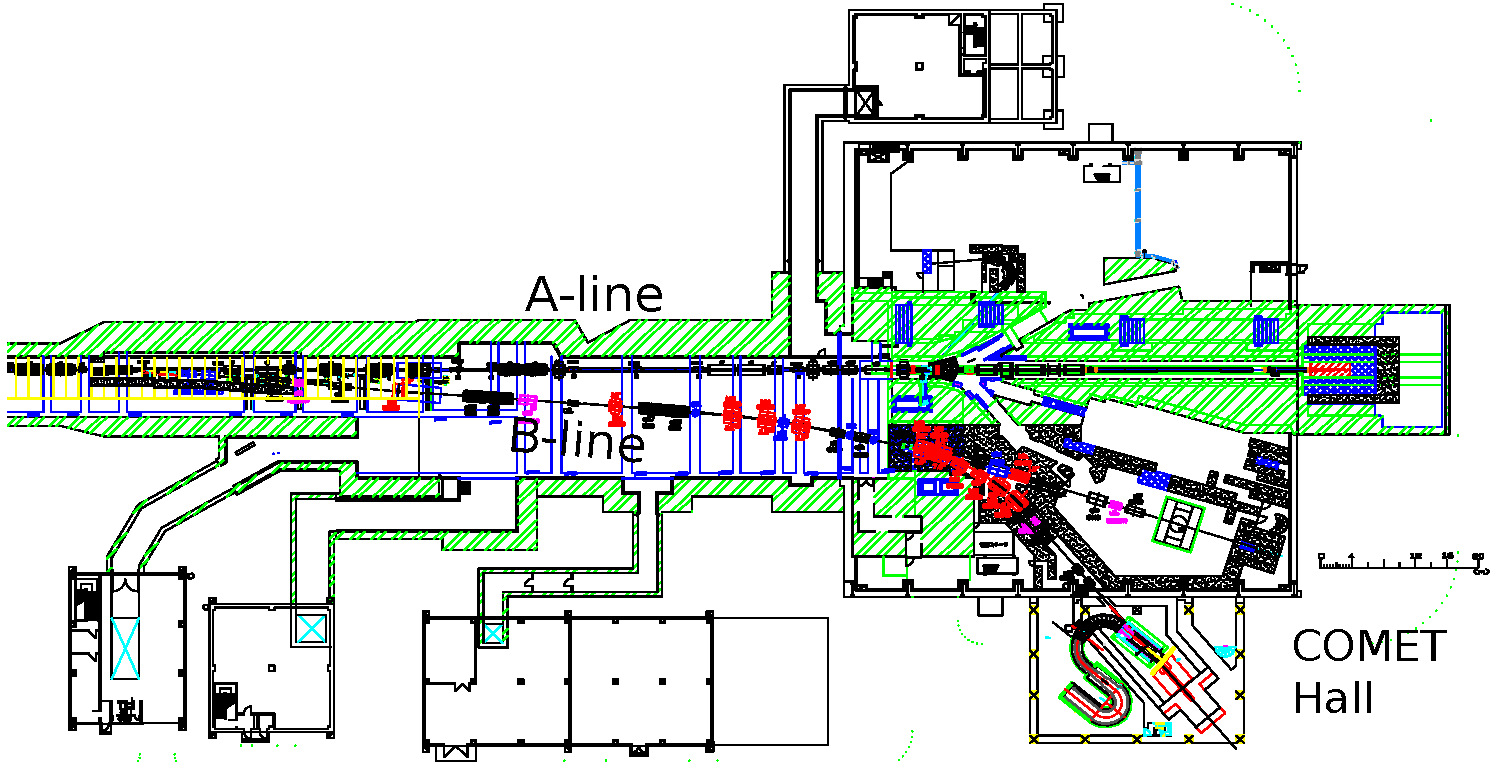
\includegraphics[scale=0.5]{chapter2/fig/beamline.pdf}
 \caption{Dedicated proton beamline for COMET experiment. A new proton beamline, B-line is under construction. COMET Hall is located beside Hadron Hall.}
 \label{bline}
\end{figure}
To accommodate the COMET experiment, a new beamline (B-line) is under construction.
As shown in figure~\ref{bline}, A-line is the existing beamline from the main ring into the Nuclear and Particle Physics (NP) Hall.
B-line is a dedicated proton for COMET experiment.

Both phase-I and phase-II require a pulsed, 8 GeV proton beam slow-extracted from the J-PARC main ring into COMET experimental hall.
The proton beam intensity and production target for phase-I and phase-II is different, which is shown as follows.
In table~\ref{intens}, the requirement of COMET is compared with Mu2e as well.
%Mu2e has a plan to operate for two years to take data, however, COMET only needs 280-day operation to reach the same sensitivity as Mu2e.
\begin{table}[H]
 \centering
 \begin{tabular}{cccccc} \hline \hline
  COMET & Target &  Beam intensity [pps] & Power [kW] & stopped muon [$\mu^-$/sec] & Sensitivity \\ \hline
  phase-I & graphite & 2.5$\times$10$^{12}$ & 3 & 1.30$\times$10$^9$ & 3.1$\times$10$^{-15}$ \\
  phase-II & tungsten & 4.4$\times$10$^{13}$ & 56 & $\textgreater$ 10$^{11}$ & $\textless$3$\times$10$^{-17}$ \\ \hline \hline
%  Mu2e & tungsten & 6$\times$10$^{12}$ & 8 & 2$\times$10$^{10}$ & $\approx$ 10$^{-16}$ \\ \hline \hline
 \end{tabular}
 \caption{Different requirement of proton beam in phase-I and phase-II.}
 \label{intens}
\end{table}


\subsection{Signal of $\mu^-N \rightarrow e^-N$ conversion}
~~~~~~When the $\mu^-N \rightarrow e^-N$ conversion is occurred, the event signal of electron is mono-energetic with energy
\begin{equation}
 E_{\mu e} = m_\mu - B_\mu - E_{rec}
\end{equation}
where $m_\mu$ and $B_\mu$ are mass of muon and bind energy of the 1s monic atom respectively.
$E_{rec}$ is the nuclear recoil energy, which is given by $E_{rec} \approx (m_\mu - B_\mu)^2/2m_N$.
It is very small and can be neglected.
The signal depends on the nuclei, for instance, it is 105.0 MeV for Al stopping target.
This mono-energtic signal is beyond the background, and one tail behind electron background can be observed in $\mu^-N \rightarrow e^-N$ conversion.

Since the muon in aluminum have lifetimes of about 864 nsec, a pulsed proton beam with interval time of 1.17 $\mu$sec is employed to eliminate the prompt background.
As shown in figure~\ref{time}, the prompt background like $\pi^-$ decay is occurred after 100 nsec beyond the proton beam.
Due to the long lifetime of muonic atoms, the time window is opened from 700 nsec to distinguish the background events and signal events.
\begin{figure}[H]
 \centering
 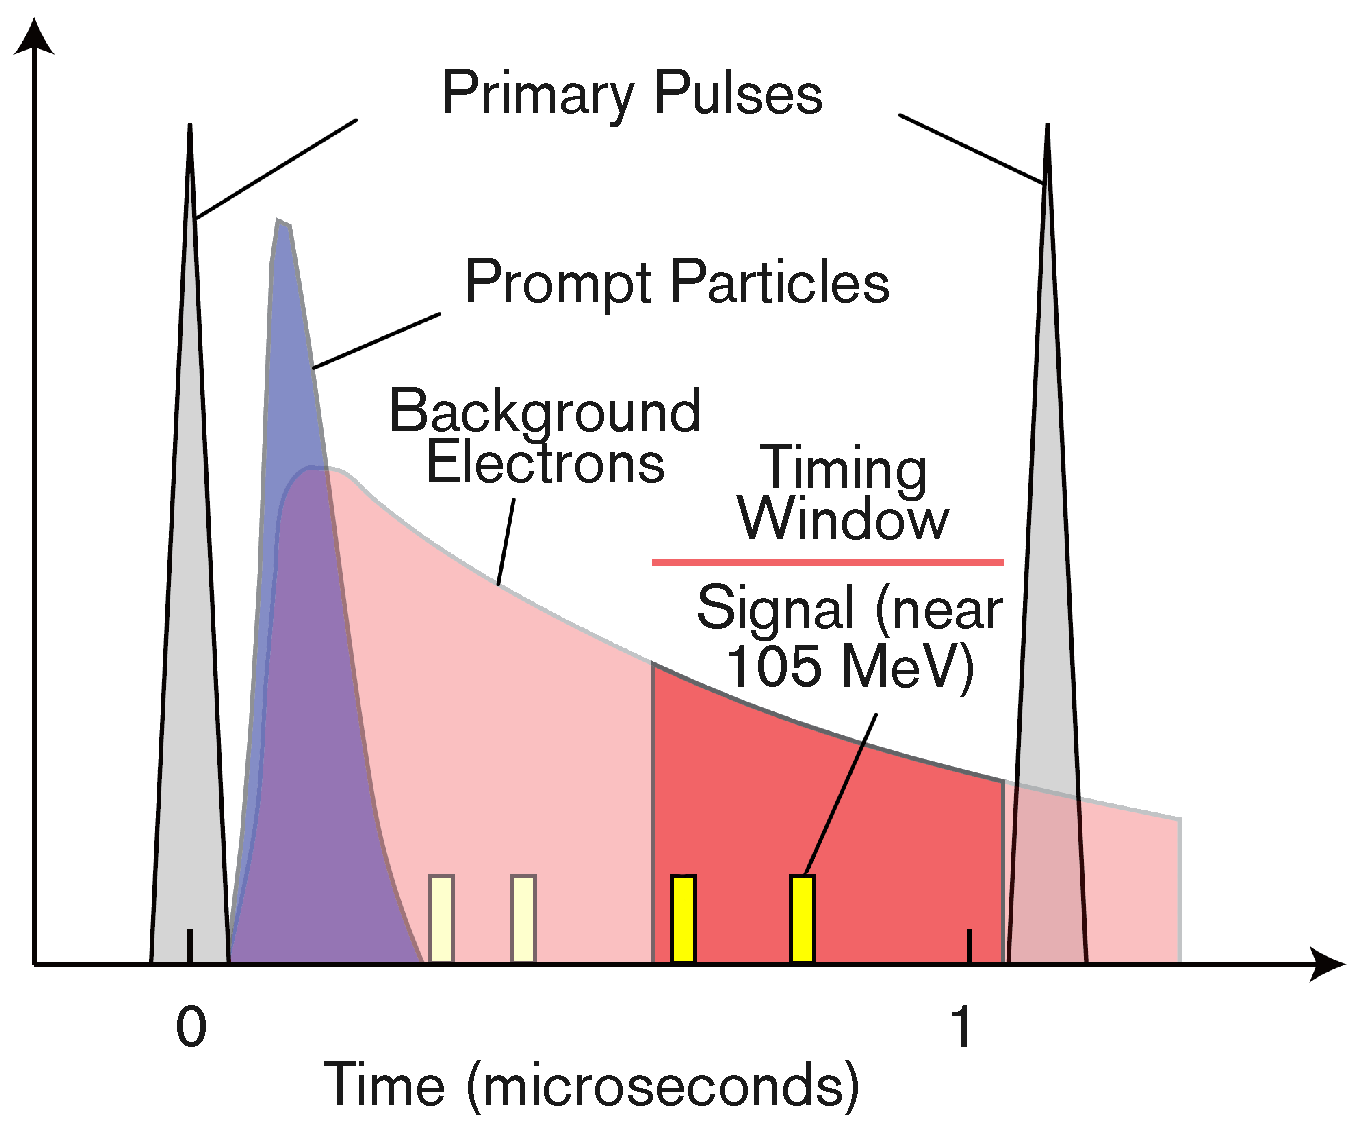
\includegraphics[scale=0.37]{chapter1/fig/time.pdf}
 \caption{The time concept of proton beam. The time window will open from 700 nsec to take data.}
 \label{time}
\end{figure}
The proton beam energy requires a pulsed beam with low production of antiproton and extinction, which will produce the backgrounds.
Therefore, the best choice is 8 GeV for COMET experiment, and the its limit intensity is 4.4$\times$10$^{13}$ pps.
Antiproton can produce the signal like electron and tracked by CDC when it hits the material.
The proton extinction factor is defined as
\begin{equation}
 R_{Ext} = \frac{N_{leak}}{N_{pulse}}
\end{equation}
where $N_{leak}$ is the proton leaked from the pulse, it becomes the background if it comes into the time window, and $N_{pulse}$ is the proton number in the pulse.

\subsection{Background of $\mu^-N \rightarrow e^-N$ conversion}
~~~~~~In COMET experiment, once a $\mu^-$ with low momentum is captured by nuclei, $\mu^-$ will transit to the ground state of 1s.
During this transition, the specific X-ray is emitted from muonic atom.
In addition, the Michel decay in orbit (DIO) emits a electron and dominates the intrinsic background of $\mu \rightarrow e$ conversion.
Without the direct background like DIO, there are many background such as beam related background listed in table~\ref{backg} will cause the indistinguishable signal in CDC during the reconstruction of signal.
\begin{table}[H]
 \centering
 \begin{tabular}{cc} \hline \hline
  Intrinsic physics backgrounds & \\ \hline
  Muon decay in orbit & $\mu^- \rightarrow e^-\nu_\mu\bar\mu_e$ \\
  Radiative muon capture (external) & $\mu^- + A \rightarrow \nu_\mu + A' + \gamma$ \\
  Radiative muon capture (internal) & $\mu^- + A \rightarrow \nu_\mu + A' + e^+ + e^-$ \\
  Neutron emission & $\mu^- + A \rightarrow \nu_\mu + A' + n$ \\
  Charged particle emission & $\mu^- + A \rightarrow \nu_\mu + A' + p (or d or \alpha)$ \\ \hline
  Beam related backgrounds & \\ \hline
  Radiative pion capture (external) & $\pi^- + A \rightarrow \gamma + A', \gamma \rightarrow e^- + e^+$ \\
  Radiative pion capture (internal) & $\pi^- + A \rightarrow e^+ + e^- + A'$ \\
  Beam electrons & $e^-$ scattering \\
  Muon decay in flight & $\mu^-$ decays in flight to produce $e^-$ \\
  Pion decay in flight & $\pi^-$ decays in flight to produce $e^-$ \\
  Neutron induced backgrounds & neutrons hit material to produce $e^-$ \\
  Anti-proton induced backgrounds & anti-proton hit material to produce $e^-$ \\ \hline
  Other background & \\ \hline
  Cosmic-ray induced background & \\
  Room neutron induced background & \\
  False tracking \\ \hline \hline
 \end{tabular}
 \caption{Potential backgrounds for searching $\mu^-N \rightarrow e^-N$ conversion.}
 \label{backg}
\end{table}

\subsubsection{Requirement of magnetic field}
Because the background depends on the muon beam quality, to eliminate the background, the muons must be captured and transported to stopping target efficiently, which can be carried out by using superconducting solenoid magnet system.
The COMET superconsucting magnets must be designed with requirements
\begin{itemize}
 \setlength{\itemsep}{-5pt} 
 \item high magnetic field around the production target to capture the pions.
 \item appropriate magnetic field to transport the low momentum muons to stopping target.
 \item low magnetic field for detector to track the signal electron.
 \item smooth magnetic field to eliminate the trapping of charged particles.
\end{itemize}
The details of magnetic field and superconducting magnet design will be explained in next chapter.

\section{Objetive}
~~~~~~The branching ratio of $\mu^- \rightarrow e^-$ conversion is predicted to around 10$^{-15}$ by the physics beyond the Standard model such as SUSY-GUT, SUSY-Seasaw.
To obtain that experimental sensitivity for searching $\mu^- \rightarrow e^-$ conversion less than 10$^{-17}$, a 8 GeV, 4.4$\times$10$^{13}$ pps proton beam is employed to produce high intense muon beam of 10$^{11}$ $\mu^-$/sec with low momentum.

As the significant part of COMET muon beamline, the pion capture solenoid in superconducting magnet system surrounds a production target with high magnetic field of 5 Tesla and small radius of 672 mm.
Its main issue is the radiation, which cause the over-heat and quench of superconducting magnet due to the thermal conductivity degradation of cooling path and stabilizer.
%which must be designed for working under the high magnetic field and high radiation environment to produce amounts of pion.
%Because the conduction cooling is employed in whole superconducting system, considering the cooling path of superconducting magnets will degrade under high radiation, in this thesis, effects of radiation on superconducting magnet and its radiation resistance have been studied.
Thus, the radiation effects on COMET superconducting solenoid are studied in this thesis.

In chapter 2, the design details of superconducting magnets for COMET phase-I experiment, pion capture solenoid, muon transport solenoid and detector solenoid, will be explained.

In chapter 3, to investigate how much radiation will be produced in COMET experiment, Monte Carlo code is modified to carry out the calculation with COMET condition.
Using the real geometry of COMET experiment, the prompt radiation for phase-II and the residual radiation after phase-I experiment is estimated.
In addition, one radiation shield is designed for protecting the superconducting coils of pion capture solenoid.

In chapter 4, the radiation resistance of the material and device, GFRPs, quench protection diode, insulation tape and pure aluminum, which are used in COMET superconducting magnet system has been tested.

In chapter 5, considering the thermal conductivity will degrade after irradiation, the most important CS1 coils where close to the production target is under risk of quench and over-heat.
Thus, the cooling and quench simulation is estimated.



  \chapter{Superconducting solenoid system for COMET experiment}
~~~~~~COMET phase-I experiment is aiming to measure the background and search the $\mu \rightarrow e$ conversion with the sensitivity of 10$^{-14}$.
Its superconducting magnet system consists of pion capture solenoid, muon transport solenoid and detector solenoid.
In phase-II experiment, nowadays' 90 degree bent transport solenoid will be extended to 180 degree curved solenoid, and another spectrometer solenoid will be added.
 
\section{Superconducting magnet system}
~~~~~~Superconducting magnet system plays a key role in pion capture, muon transport and signal tracking.
In the case of COMET phase-I experiment, the 8 GeV proton with high intensity is injected into superconducting magnet and hits the target to produce pion, then these backward pions are captured by pion capture solenoid, which provides 5 Tesla magnetic field at peak.
\begin{figure}[H]
 \centering
 \includegraphics[scale=0.45]{chapter2/fig/solenoid.pdf}
 \caption{Schematic layout of superconducting magnet system for COMET phase-I experiment.}
 \label{solenoid}
\end{figure}
Muons with low momentum from the decay of captured pions are transported to stopping target by the muon transport solenoid with 3 Tesla.
Because the high momentum muon and the other particles will cause the background on detector, the muon transport solenoid is designed with 90 degree curve to throw out these particles.
After the muon captured by stopping target, the emitted electron from stopping target will be bent by detector solenoid which provides 1 Tesla magnetic field and tracked in cylindrical drift chamber (CDC).

The schematic layout of COMET superconducting solenoid is given in figure~\ref{solenoid}.
Pion capture solenoid consists of CS0, CS1, MS1, MS2 and TS1a-TS1f superconducting coils.
Meanwhile, muon transport solenoid includes TS2, TS3 and BS coils, and detector solenoid has 12 DS coils.

 \section{Pion capture solenoid}
~~~~~~Pion capture solenoid is most critical magnet for capturing the pions from production target with a large solid angle.
Considering the valleys of magnetic field causes the trapping of charged particle, the magnetic field distribution must be smooth.
The details of the magnetic field of pion capture solenoid is shown in table~\ref{magfldcs}.
\begin{table}[H]
 \centering
 \begin{tabular}{ccccccc} \hline \hline
  Coils & B$_z$ & Inner radius & Outer radius & Length & Current & Current density \\
   & [T] & [mm] & [mm] & [mm] & [A] & [A/mm$^2$] \\ \hline
  CS0 & 4.0 & 662 & 806 & 175 & 2700 & 33.75 \\
  CS1 & 5.0 & 662 & 806 & 1350 & 2700 & 33.75 \\
  MS1 & 4.0 & 662 & 742 & 1425 & 2700 & 33.75 \\
  MS2 & 3.0 & 662 & 774 & 700 & 2700 & 33.75 \\
  TS1a & 3.0 & 250 & 266 & 200 & 2700 & 33.75 \\
  TS1b & 3.0 & 250 & 298 & 240 & 2581 & 32.26 \\
  TS1c & 3.0 & 250 & 314 & 200 & 2700 & 33.75 \\
  TS1d & 3.0 & 250 & 314 & 200 & 2619 & 32.74 \\
  TS1e & 3.0 & 250 & 298 & 200 & 2538 & 31.73 \\
  TS1f & 3.0 & 400 & 496 & 350 & 2916 & 36.45 \\ \hline \hline
 \end{tabular}
 \caption{Details of coils for pion capture solenoid.}
 \label{magfldcs}
\end{table}
All of the superconducting coils in pion capture solenoid is connected together with the same current provided by one power supply.
Furthermore, conduction cooling is employed in whole COMET superconducting magnet system due to the tritium production under high radiation environment by reaction of $^3$He(n,p)$^3$H.
Also the direct cooling needs helium vessel and the coils must be enlarged, the more radiation and stored energy deposits in larger coils.
From all aspect, the conduction cooling is the best choice for COMET superconducting magnet system.
aluminium-stabilized conductors is used in all the coils for reducing the heat load and preventing the over heat of coils after quench.

\subsection{Coils structure}
~~~~~~To reduce the energy deposition in coils, superconducting wires are all merged with 5N aluminium (0.1\% Ni) due to its low density.
The reason why 
0.1\% nickel is mixed to enhance the mechanical property of conductor.
\begin{figure}[H]
 \centering
 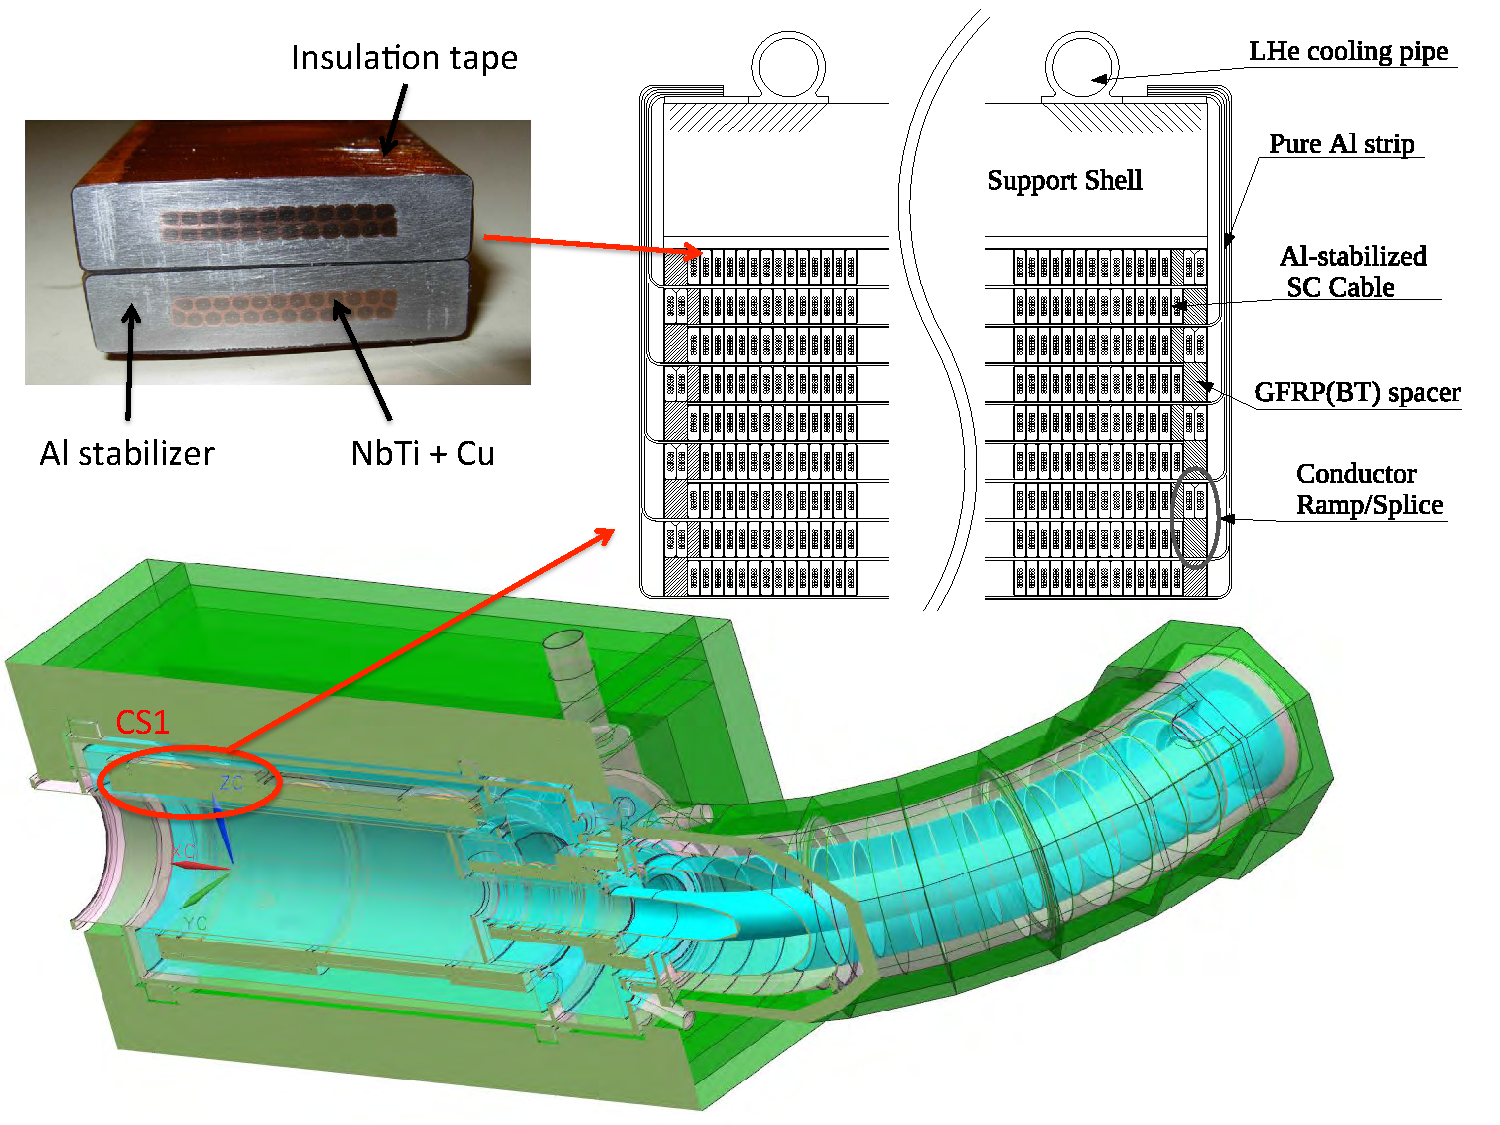
\includegraphics[scale=0.45]{chapter2/fig/coil.pdf}
 \caption{ Coil and conductor structure of CS1.}
 \label{cssrtu}
\end{figure}

The aluminium-stabilized conductor with the size of 15.0 $\times$ 4.7 mm$^2$ is wound with two layers of insulation tape, which is made of polyimide film covered by boron free glass with BT and epoxy resin.
Here, The reason why BT and epoxy resin is used because it has good mechanical property under the high radiation.
In addition, the insulated conductor is impregnated by the BT and epoxy resin mixed with silica filler during the coils winding.

The coil structure of CS1 and detail of design parameters are shown in figure~\ref{cssrtu} and table~\ref{desip} respectively.
There are 9 layers superconducting coils totally, and each layer is cooled by inserting 1 mm thick pure aluminium strip with RRR of 2000.
Each aluminium strip is installed between two conductor layers, and connected to the liquid helium cooling pipe.
Support shell with 5 cm thick is located on the top of superconducting coils to suppress the deformation of coils.
\begin{table}[H]
 \centering
 \begin{tabular}{ll} \hline \hline
  Item & Value \\ \hline
  Conductor & aluminium stabilized SC cable \\
   & Al:Cu:NbTi = 7.3:0.9:1 \\
  Cable dimensions & 15.0 $\times$ 4.7 mm$^2$ (without insulation) \\
   & 15.3 $\times$ 5.0 mm$^2$ (with insulation) \\
  Cable insulation & Polyimide film/Boron-free glass cloth \\
   & /BT-epoxy prepreg \\
  Magnet length & $\sim$ 6 m \\
  Number of coils & 10 \\
  Operation current & 2700 A \\
  Max. field on conductor & 5.5 T (T$_{cs}$ = 6.5 K) \\
  Stored energy & 47 MJ \\
  Coil layer & 9 (CS0+CS1), 5 (MS1), 7 (MS2), \\
   & 1$\sim$6 (TSa$\sim$TS1f) \\
  Quench protection & NA \\ \hline \hline
 \end{tabular}
 \caption{Details of design parameters for capture solenoid magnet.}
 \label{desip}
\end{table}

\subsection{Production target}
~~~~~~Production target is to make amounts of pions in the capture solenoid.
Phase-I is going to use the IG-43 graphite target rod with length of 60 cm, radius of 2 cm and density of 1.82 g/cm$^3$.
3.2 kW proton beam will deposit a heat load of approximately 100 W in the graphite target.
The temperature of target grows up to 190$^{\circ}$C at peak when 100 W energy is deposited in target.
A target support system accurately locates the target within the solenoid inner shield.

To achieve more pion production in COMET phase-II experiment, the target will be changed to pure tungsten rod with length of 16 cm and radius of 0.3 cm after the implementation of phase-I.
In addition, due to 56 kW proton beam power, phase-II target must be cooled on low temperature.
The proton beam also has to be fitted to a gaussian beam with 0.2 cm radius.

\subsection{Radiation shield}
~~~~~~A radiation shield is installed inside the CS and MS coils to protect superconducting coils from radiation.
This radiation shield has to be designed for both phase-I and phase-II experiment due to the high residual radiation.
The neutron came from production target directly is about 3$\times$10$^{12}$ n/cm$^2$/sec in COMET phase-II experiment, which corresponds to 10$^{24}$ n/m$^2$.
Both NbTi superconducting cable and stabilizers degrade if they are irradiated by neutrons with this order.
Therefore, due to a small radius of capture solenoid, a powerful radiation shield is needed to stop or decrease the radiation in short distance.
The most ideal radiation shield is made of pure tungsten with density of 19.25 g/cm$^3$.

However, to reduce the costs, a new composited radiation shield is designed and the details will be described in next chapter.

\subsection{Quench protection system}
~~~~~~Quench is caused by a hot spot in superconducting magnet.
When a hot spot quenches, temperature will rise suddenly, and propagate to all magnet.
Superconducting magnets has a risk of burn-out at temperature of quench.

Because the current becomes the joule heat after quench, decreasing the current quickly can suppress the temperature rise after quench.
There are two ways to speed up the current decay.
As shown in figure~\ref{dump}, one is to use the dump resistor in superconducting magnet circuit.
Once the quench is detected, the power supply will be turned off and current will flow towards to the dump resistor.
One quench protection diode is a switch for the quench protection circuit.
It is connected with superconducting wire and cooled to 4.2 K during operation.
The time constant is written as
\begin{equation}
 \tau = \frac{L}{R_{dump}}
\end{equation}
where $L$ is the inductance of magnets and $R_{dump}$ is the resistance of dump resistor respectively.
Higher resistance of dump resistor makes current decay quicker.
In the case of the pion capture solenoid, it is covered by the aluminium stabilizer.
Once quench is occurred, the current will flow into the aluminium stabilizer and copper matrix.
The current must decay more quickly due to the self resistance of stabilizer and matrix.
The time constant is written as
\begin{equation}
 \tau = \frac{L}{R_{dump} + R_{self}}
\end{equation}

Another way is to make the superconducting magnet quench to increase the self resistance by external heater.
It needs external power supply to heat the heater.
\begin{figure}[H]
 \begin{subfigure}{0.3\textwidth}
 \centering
 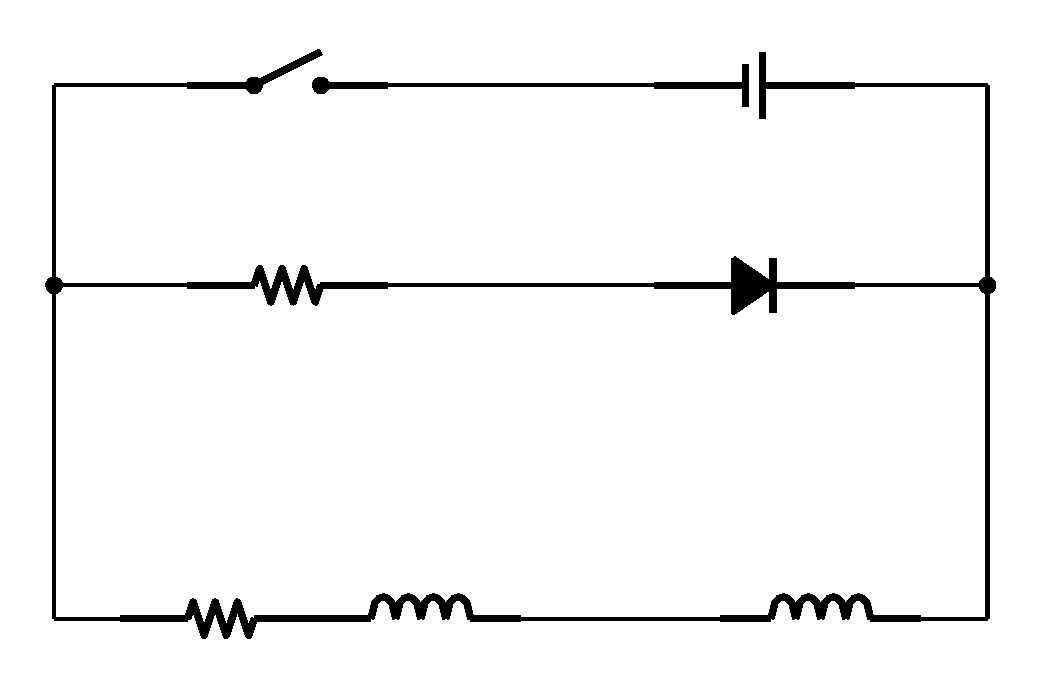
\includegraphics[scale=0.4]{chapter2/fig/dump.pdf}
 \end{subfigure}
 \hspace{0.2\textwidth}
 \begin{subfigure}{0.3\textwidth}
 \centering
 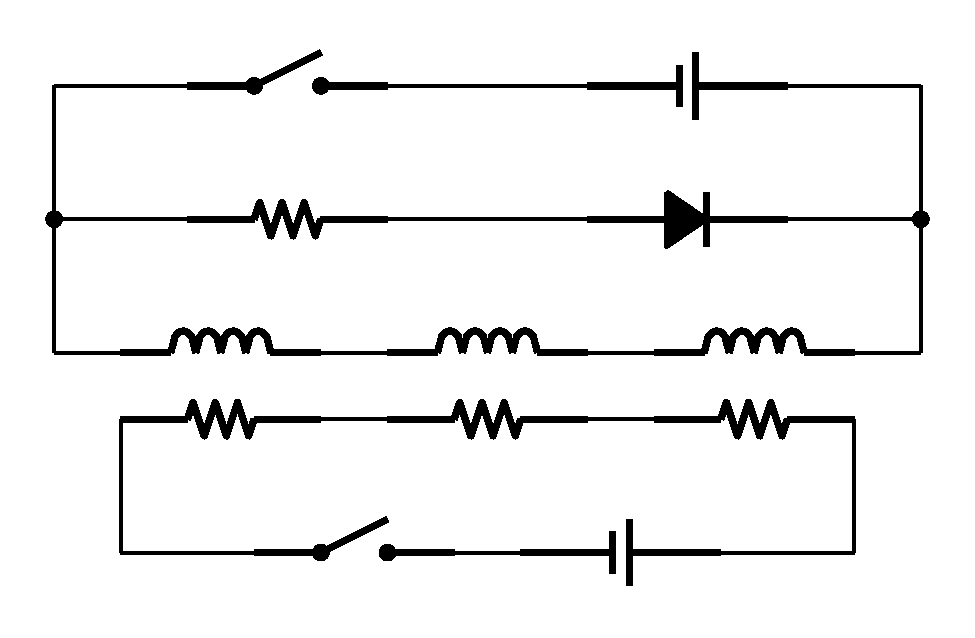
\includegraphics[scale=0.4]{chapter2/fig/heater.pdf}
 \end{subfigure}
 \caption{Schematics of quench protection circuit.}
 \label{dump}
\end{figure}

The quench protection system for pion capture solenoid is shown in figure~\ref{capture}.
All superconducting magnets in pion capture solenoid are connected together.
The power supply for capture solenoid is 2700 A, and 4 reserve trim power supplies and dump resistors are to reduce the current for TS1b, TS1d, TS1e and TS1f.
A dump resistor for capture solenoid is 0.185 $\Omega$, supposed the power supply is 500 V.
Once quench is occurred in one of the superconducting magnet of pion capture solenoid, the power supply will be turned off, and quench back heater will heat the all magnets.
Total resistivity of pion capture solenoid increases after heated, thus, the current will decay to zero in 1 min.
\begin{figure}[H]
 \centering
 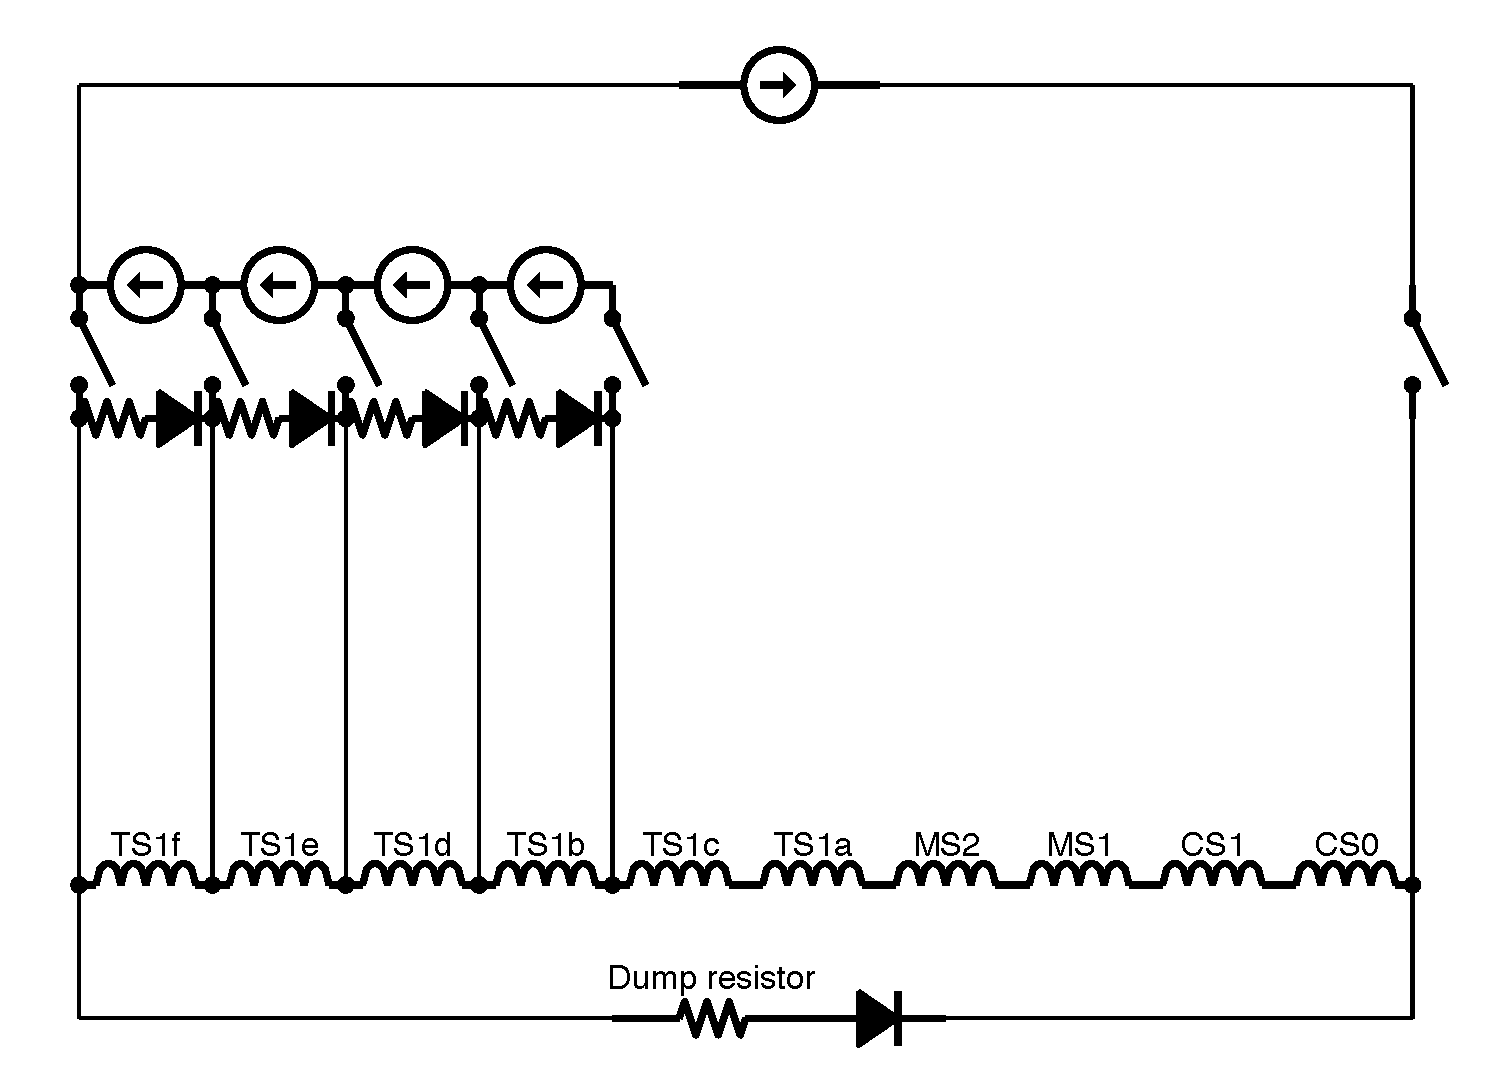
\includegraphics[scale=0.4]{chapter2/fig/capture.pdf}
 \caption{Schematics of quench protection system for pion capture solenoid.}
 \label{capture}
\end{figure}

 \section{Muon transport solenoid}
~~~~~~Muons are transported to the stopping target through the muon transport solenoid, which consists of curved superconducting magnets.
The muon transport solenoid must be designed to select the muons with low momentum and eliminate muons with high momentum ($p_{\mu^-} \textgreater$ 75 MeV/c), in addition, it also must be long enough for the pion decay.
Due to the beam dispersion in muon transport solenoid, the selection of charged particle depends on their momentum.
The magnitude of drift is given by
\begin{equation}
 D = \frac{1}{qB}(\frac{s}{R})\frac{p_L^2 + p_T^2/2}{p_L} = \frac{1}{qB}(\frac{s}{R})\frac{p}{2}(cos\theta + \frac{1}{cos\theta})
\end{equation}
where $q$ is the electric charge of particle, $B$ is the magnetic field, $s$ and $R$ are the path length and the radius of curvature of solenoid respectively.
$s/R$ is the bending angle, $p_L$ and $p_T$ [GeV/c] are longitudinal and transverse momentum.
To keep the center of the helical trajectories of muons in the bending plane, a compensating dipole field parallel to the drift direction is applied, which is given by
\begin{equation}
 B_{comp} = \frac{1}{qR} \frac{p_0}{2} (cos\theta_0 + \frac{1}{cos\theta_0})
\end{equation}

The muon transport solenoid consists of 16 coils without stabilizer and a dipole coil with 0.056 Tesla compensating field is attached on the outer surface of each solenoid.
Details of each coil and design parameters are listed in table~\ref{tscoil} and \ref{designts}.
\begin{table}[H]
 \centering
 \begin{tabular}{ll} \hline \hline
  Item & Value \\ \hline
  Conductor & NbTi/Cu wire \\
   & Cu:NbTi = 6:1 \\
  Cable dimensions (solenoid) & $\phi$ 1.5 mm (without insulation) \\
   & $\phi$ 1.56 mm (with insulation) \\
  Cable dimensions (dipole) & $\phi$ 1.2 mm (without insulation) \\
   & $\phi$ 1.3 mm (with insulation) \\
  Cable insulation & Polyimide-imide enamel (AIW), \\
   & PVF (TS2-15, TS3) \\
  Magnet length & $\sim$ 6 m \\
  Curvature radius & 3 m \\
  Number of solenoid coils & 18 \\
  Number of dipole coils & 16 pairs \\
  Operation current & 210 A (solenoid) \\
   & 165 A (dipole) \\
  Field on axis & $\sim$ 3 T (solenoid) \\
   & $\sim$ 0.056 T (dipole) \\
  Stored energy & 5.6 MJ \\
  Total inductance & 254 H \\
  Refrigeration & conduction from forced flow 2-phase \\
   & LHe piping (7-10 g/sec) \\
  Quench protection & semi-active quench back heater \\ \hline \hline
 \end{tabular}
 \caption{Design parameters of transport solenoid.}
 \label{designts}
\end{table}

\begin{table}[H]
 \centering
 \begin{tabular}{cccccccc} \hline \hline
  Coil & B$_z$ & B$_y$ & Length & Inner radius & Outer radius & Current & Current density \\
   & [T] & [T] & [mm] & [mm] & [mm] & [A] & [A/mm$^2$] \\ \hline
  TS2a & 3 & NA & 255 & 234 & 249 & 210 & 72 \\
  TS2-1 & 3 & 0.06 & 205 & 234 & 264 & 210 & 95 \\
  TS2-2$\sim$15 & 3 & 0.06 & 205 & 234 & 272 & 210 & 95 \\
  TS2-16 & 3 & 0.06 & 205 & 234 & 254 & 210 & 94 \\
  TS3 & 3 & NA & 600 & 400 & 437 & 190 & 85.5 \\ \hline \hline
 \end{tabular}
 \caption{Coils parameters for muon transport solenoid.}
 \label{tscoil}
\end{table}



\section{Detector solenoid}
~~~~~~The detector solenoid consists of 14 DS coils and 5 BS collimator coils with 1 and 1.57 Tesla magnetic field respectively.
The superconducting wires of BS and DS have diameter of 1.26 mm with copper ratio of 4.2, and RRR of copper is higher than 60.
Superconducting cable is insulated by PVF with 30 $\mu$m thick.
The stored energy of DS and BS are about 4.45 MJ and 0.166 MJ respectively.
Inductance of these two solenoids are 240 H and 13.8 H.
The detector solenoid is cooled by GM refrigerators independently.
%\begin{table}[H]
% \centering
% \begin{tabular}{cccccccc} \hline \hline
%  Coil & B$_x$ & Length & Inner radius & Outer radius & Location & Current & Current density \\
%   & [T] & [mm] & [mm] & [mm] & [mm] & [A] & [A/mm$^2$] \\ \hline
%  BS1 & 1.57 & 300 & 230 & 241.1 & 10382.39 & 155 & 111 \\
%  BS2 & 1.57 & 150 & 230 & 245.5 & 10657.39 & 155 & 111 \\
%  BS3 & 1.57 & 240 & 310 & 320 & 10902.39 & 155 & 111 \\
%  BS4 & 1.57 & 180 & 310 & 320 & 11162.39 & 155 & 111 \\
%  BS5 & 1.57 & 180 & 310 & 320 & 11422.39 & 155 & 111 \\
%  DS1 & 1 & 170 & 1070 & 1078 & 11397.39 & 191 & 131 \\
%  DS2 & 1 & 170 & 1070 & 1078 & 11607.39 & 191 & 131 \\
%  DS3 & 1 & 170 & 1070 & 1078 & 11817.39 & 191 & 131 \\
%  DS4 & 1 & 170 & 1070 & 1078 & 12027.39 & 191 & 131 \\
%  DS5 & 1 & 170 & 1070 & 1078 & 12237.39 & 191 & 131 \\
%  DS6 & 1 & 170 & 1070 & 1078 & 12447.39 & 191 & 131 \\
%  DS7 & 1 & 170 & 1070 & 1078 & 12657.39 & 191 & 131 \\
%  DS8 & 1 & 170 & 1070 & 1078 & 12867.39 & 191 & 131 \\
%  DS9 & 1 & 170 & 1070 & 1078 & 13077.39 & 191 & 131 \\
%  DS10 & 1 & 170 & 1070 & 1078 & 13287.39 & 191 & 131 \\
%  DS11 & 1 & 170 & 1070 & 1078 & 13497.39 & 191 & 131 \\
%  DS12 & 1 & 170 & 1070 & 1078 & 13707.39 & 191 & 131 \\
%  DS13 & 1 & 170 & 1070 & 1078 & 13917.39 & 191 & 131 \\
%  DS14 & 1 & 170 & 1070 & 1078 & 14127.39 & 191 & 131 \\ \hline \hline
% \end{tabular}
% \caption{Dtails of coil for the collimator and detector solenoids.}
% \label{dsbs}
%\end{table}



  \chapter{Radiation estimation}
~~~~~~Since the high energy and high intensity proton beam is used in COMET experiment, the radiation is an important issue for superconducting magnet design.
In this chapter, the details of prompt and residual radiation will be described.
Moreover, one radiation shield is designed for protecting the pion capture solenoid.

 \section{Hadronic models}
~~~~~~Monte Carlo code is usually used in high energy physics to simulate the physical process.
Recently, it is also playing increasingly role in the other studies, like heavy ion therapy~\cite{therapy}, nuclear fusion reactor et al.
The hadron model in some Monte Carlo codes which is used in the paper is introduced as follows.

  \subsection{PHITS}
~~~~~~Particle and Heavy Ion Transport code System (PHITS) is developed by Japan Atomic Energy Agency (JAEA)~\cite{phits}.
The PHITS code is written in FORTRAN, and it can deal with the transport of almost all particles over a wide energy range. 
\begin{figure}[H]
 \centering
 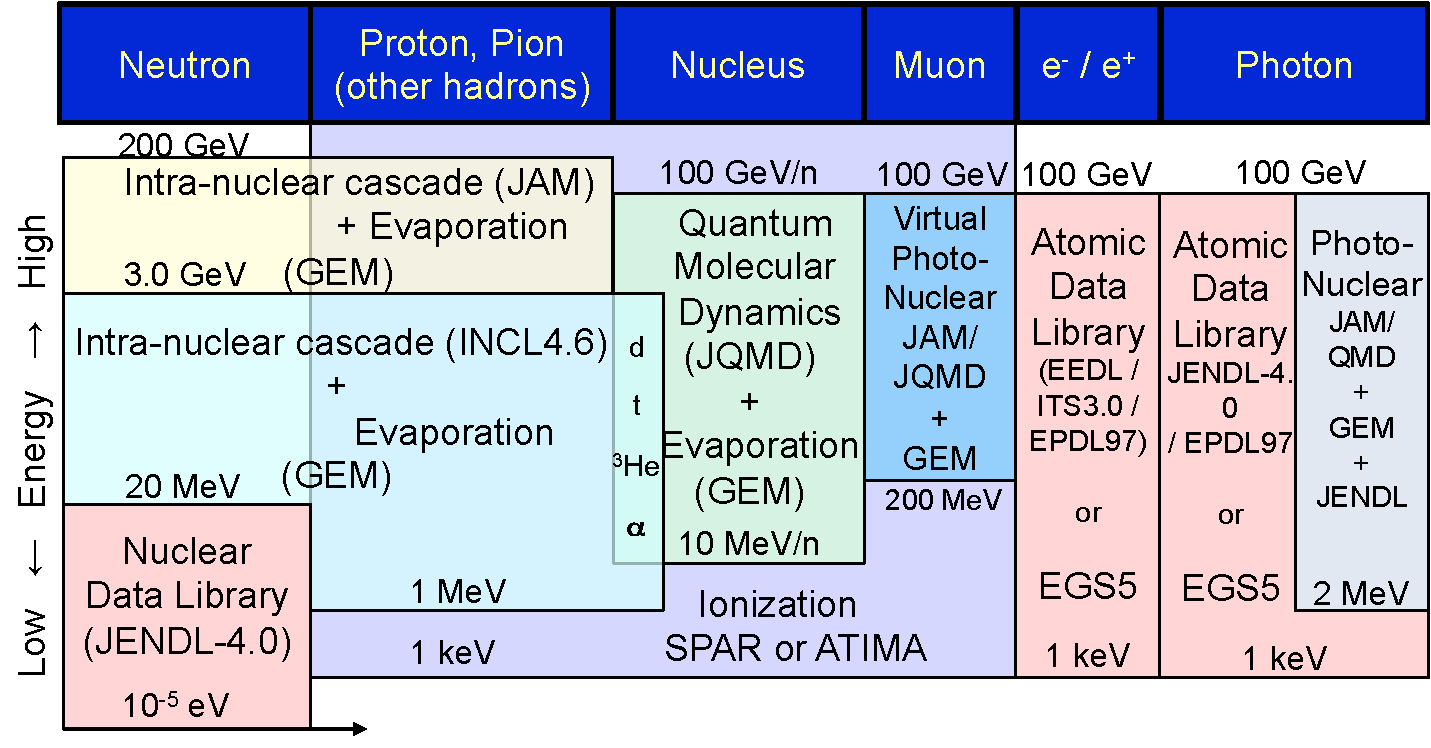
\includegraphics[scale=0.43]{chapter3/fig/physicalmodel.pdf}
 \caption{The physical model used in PHITS code. Default hadronic model is JAM\_INCL4.6\_JENDL, moreover, JAM\_BERT\_JENDL and JAM\_INC-ELF\_JENDL are able to be selected in PHITS code.}
 \label{phitsmodel}
\end{figure}
PHITS uses its own models for nuclear collisions and for hadron reactions.
The details of physical model in PHITS are shown in figure~\ref{phitsmodel}.
As for 8 GeV hadron collision, the Japanese nuclear library, JENDL-4.0, is employed in the low energy region ($\le$20 MeV).
Between 20 MeV and 3 GeV, there are three kinds of different model in hadron reaction, which are the INCL4.6~\cite{incl}, Bertini and INC-ELF~\cite{incelf}.

  \subsection{FLUKA}
~~~~~~FLUKA is a fully integrated particle physics Monte Carlo simulation package developed by CERN~\cite{fluka}.
Two hadronic models is included in FLUKA, the Generalized IntraNuclear Cascade (GINC) model in high energy region ($\ge$ 5 GeV) which is treated in the Glauber-Gribov formalism and PEANUT model in the low energy region~\cite{fluka2}.

  \subsection{GEANT4}
~~~~~~GEANT4 is the most powerful toolkit for simulation of high energy physics experiment~\cite{geant4}.
Like PHITS, GEANT4 is using the G4 neutron data library (G4NDL) in the energy less than 20 MeV.
Between 20 MeV and 5 GeV, three models, Binary, Bertini and INCL++, can be selected in G4.
G4 also provides the FTF String model from the range of 5 GeV to 20 TeV and QG String model to 100 TeV.
%\begin{table}[H]
% \centering
% \begin{tabular}{lcrr} \hline
%  Procss & MARS & GEANT4 & PHITS \\ \hline \hline
%  $\mu$ capture & Modified Fermi-Teller Law & None & CHIPS \\ \hline
%  $\pi$ capture & Modified Fermi-Teller Law & INCL 4.6 & QGSP\_BERT 4.0 \\ \hline
%  Radiative $\mu$ capture & & & CHIPS \\ \hline
%  Low energy hadron production & CEM95 & BERT, INCL4.6, INC-ELF & BERT\_HP \\ \hline
% \end{tabular}
%\end{table}

 \section{Modification of PHITS code}
~~~~~~Here, the modification of PHITS code will be introduced to achieve the realastic simualtion of COMET experiment.
The main optimization of PHITS code is listed as follows.
\begin{itemize}
 \setlength{\itemsep}{-5pt}
 \item Bridged PHITS and the accelerator simulation code TURTLE.
 \item Enable to read the external field map.
 \item The charged particle can be bended in user defined field.
 \item The output file from PHITS can be read into GEANT4 code.
 \item Enable to use the ROOT toolkit in PHITS.
\end{itemize}

 \subsection{Proton beam}
The proton beam source is simulated by the accelerator simulation code, called TURTLE in COMET experiment.
The simulation of TURTLE has been already shown in figure~\ref{beam}, and one bunch of the proton beam where locates in front of production target is gaussian distribution with size of 2 cm $\times$ 0.8 cm and momentum of 8.9 MeV/c.
PHITS can read the external file as the radiation source, but due to the different coordinate used in PHITS and TURTLE.
One script has been written to convert the coordinate and pretend the PHITS dump file to be read. 
The proton beam used in radiation estimation is TURTLE data for phase-I and gaussian beam for phase-II, respectively.
\begin{figure}[H]
 \centering
 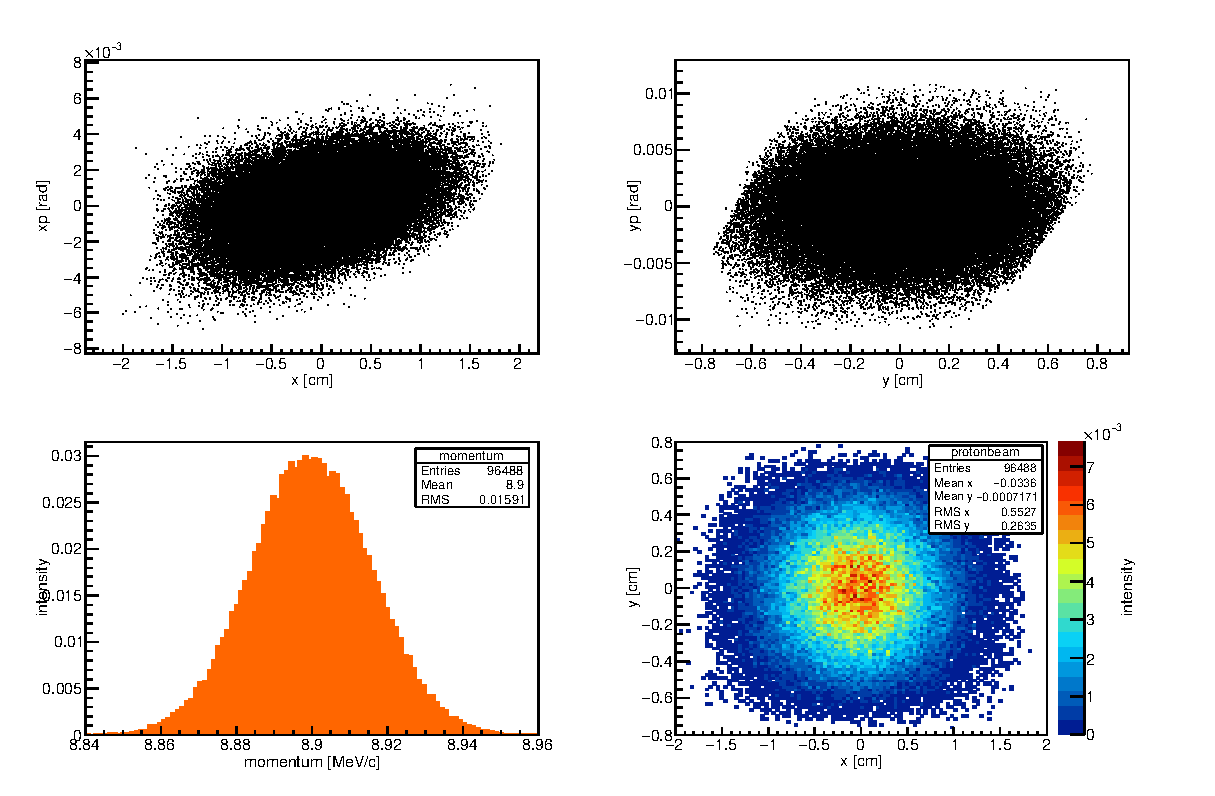
\includegraphics[scale=0.5]{chapter3/fig/beam.eps}
 \caption{Proton beam distribution simulated by TURTLE code. Top two are the momentum distribution of x and y axis, respectively. Bottom two are the momentum distribution and spatial distribution. Here, intensity means the normalized intensity.}
 \label{beam}
\end{figure}
 
 \subsection{Magnetic field}
~~~~~~As for nowadays' PHITS, it still cannot bend the charged particles in user's field map.
However, the radiation estimation is affected by the magnetic field sensitively.
To solve this issue, one magnetic field interpolation subroutine written by C is compiled with FORTRAN files.
The details of the magnetic field interpolation is described in appendix A.
The charged particles are bended with a circular path in the magnetic field which is written as
\begin{equation}
 R = \frac{p}{eB} = \frac{m\gamma \beta c}{eB} = p \cdot \frac{3.336}{B}
\label{beq}
\end{equation}
To enesure the magnetic field interpolation, the uniform field map with 5 Tesla has been tested and the tracking is shown in~\ref{2uniform}.
Following the equation~\ref{beq}, the bending radius of 0.1 GeV/c momentum electron in 5 Tesla is 6.6 cm.
The radius from the simualtion is totally agree with the calculation.
 \begin{figure}[H]
  \centering
  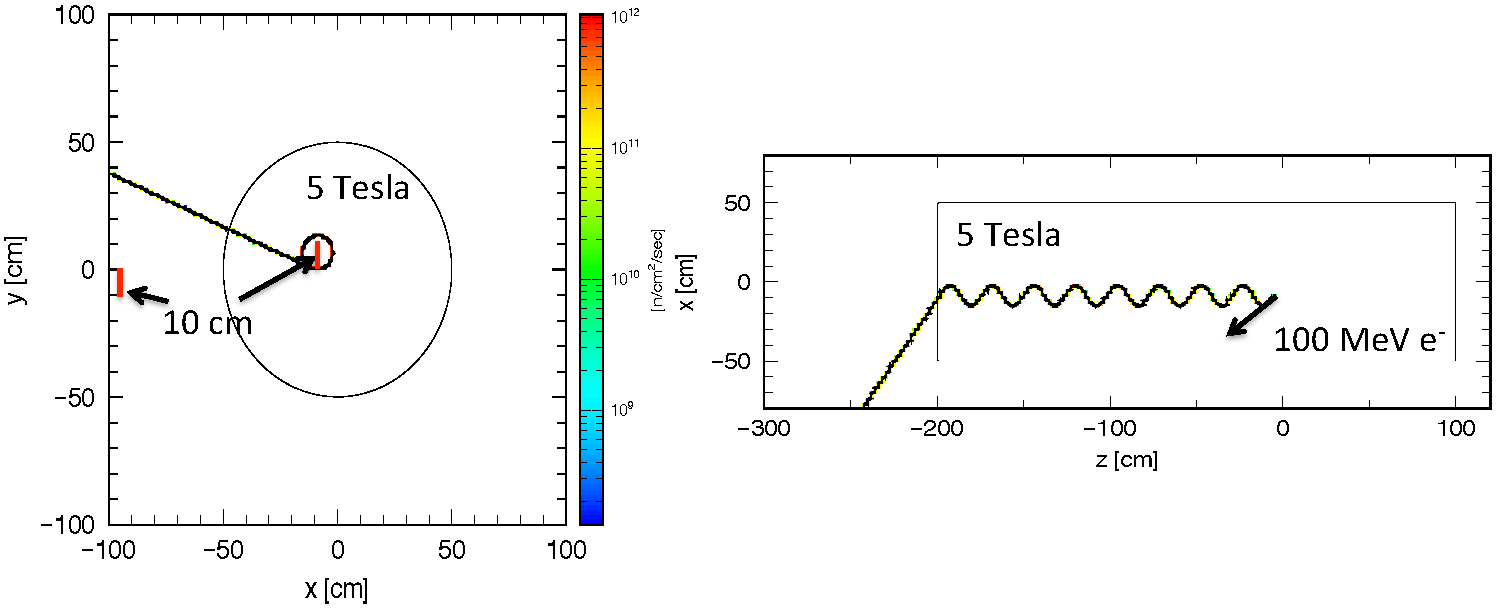
\includegraphics[scale=0.45]{chapter3/fig/magtest.pdf}
  \caption{Tracking of 100 MeV electron with uniform 5 Tesla field. One electron is injected with angle of 30 degree. Magnetic field is applied in a cylinder with radius of 50 cm and length of 300 cm.}
  \label{2uniform}
 \end{figure}
The field map included into COMET PHITS simulation is calculated by Finite Element Method (FEM) with iron yoke, which is shown in figure~\ref{field}.
There are still some missing part of field map, like the field around the iron yoke and proton beam transport pipe.
It will affect the proton beam transportation definitely, but this map is enough for the radiation study.

 \begin{figure}[H]
  \begin{subfigure}{0.3\textwidth}
   \centering
   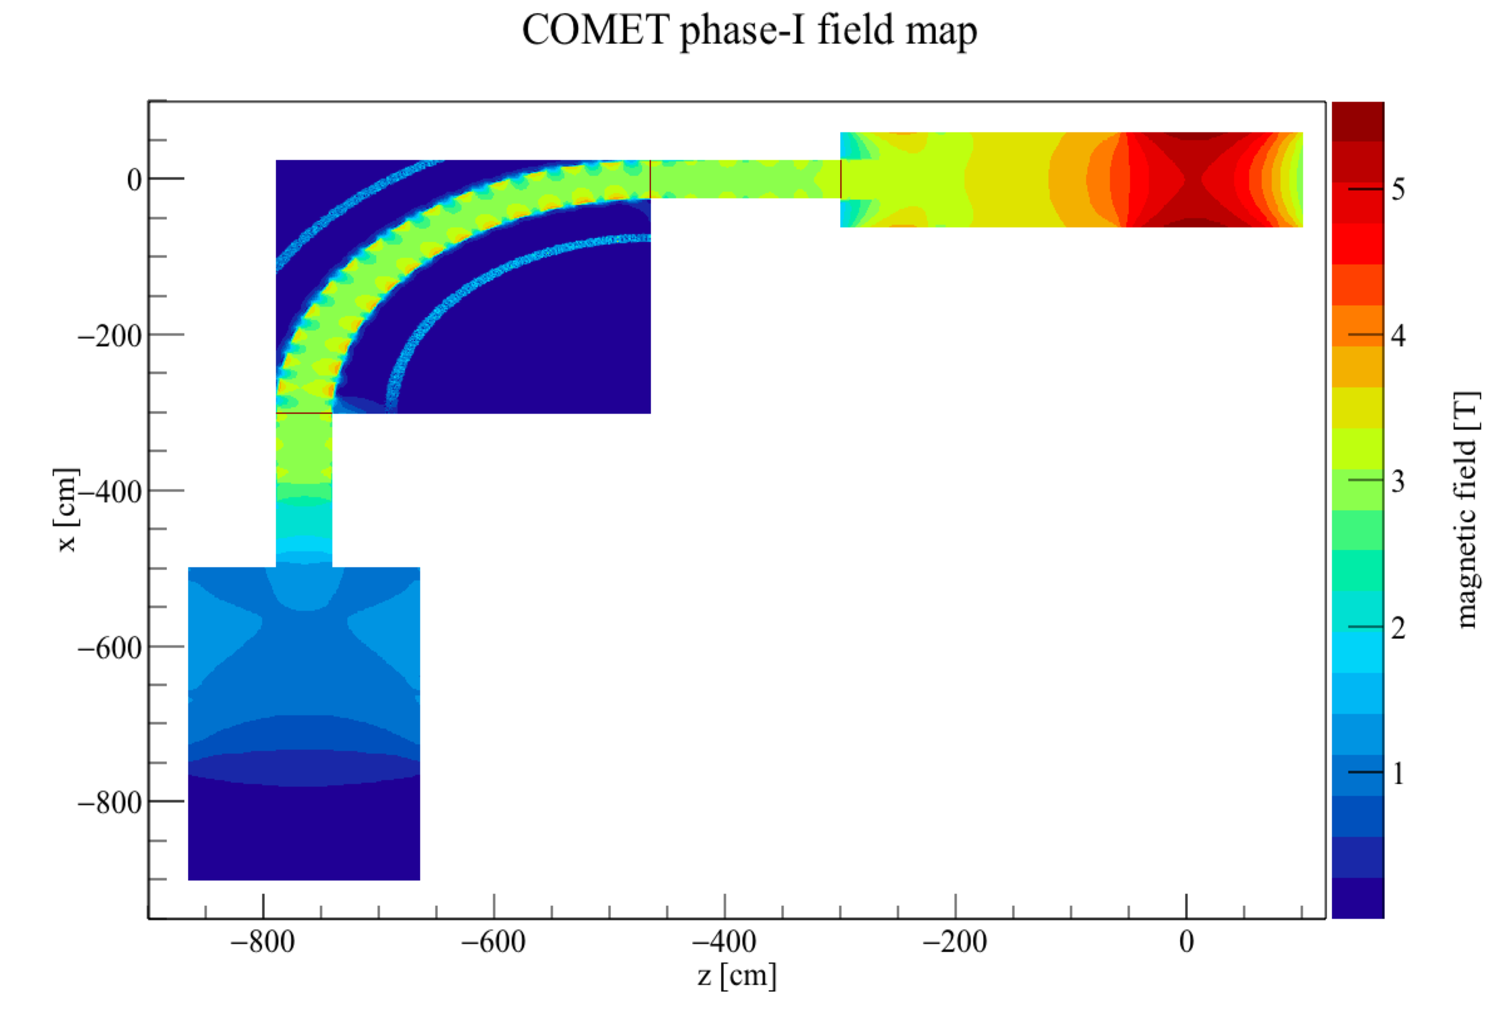
\includegraphics[scale=0.32]{chapter3/fig/fieldmap.pdf}
  \end{subfigure}
  \hspace{0.2\textwidth}
  \begin{subfigure}{0.3\textwidth}
   \centering
   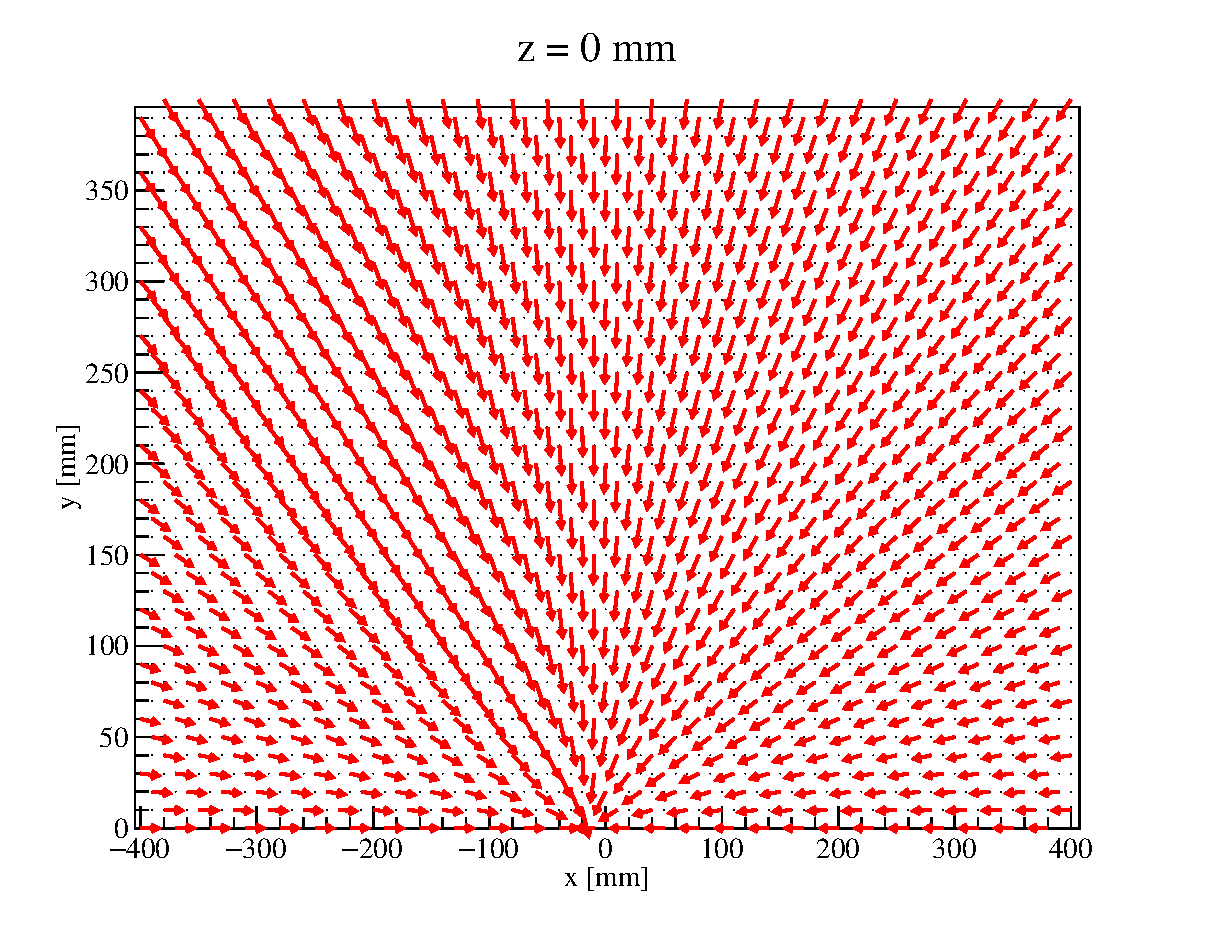
\includegraphics[scale=0.35]{chapter3/fig/fieldxy}
  \end{subfigure}
  \caption{Magnetic field map of phase-I experiment used in PHITS simulation. It is calculated by FEM with iron yoke. Mangetic field vector at z = 0 cm is shown on the right.}
  \label{field}
 \end{figure}

 \section{Prompt radiation}
  \subsection{Physical model comparison}
~~~~~~Since PHITS does not include a lot of physics model involved muon such as muon decay on the orbits, specific X-ray of muon capture, rate decay of muon et al., on the other hand, GEANT4 physics model is almost implement compared to PHITS, the comparison of particle yield between GEANT4 and PHITS is necessary to make sure the missing physics model can be neglected in radiation estimation.

The comparison is taken by using a very simple geometry, which is only one graphite target with 60 cm length and 2 cm radius.
Incident proton beam is 8 GeV with gaussian distribution.
Magnetic field is included in the region around target with 30 cm radius and 140 cm length.
As the result shown in figure~\ref{model} and table~\ref{2model}, the integral yield of pion and muon from target predicted by PHITS is higher than GENAT4's with factor 12.9\%.
For the neutron, the production yield has 17\% difference between GEANT4 and PHITS.
\begin{table}[H]
 \centering
 \begin{tabular}{cccccc} \hline \hline
  & $\mu^-$ [n/proton] & $\pi^-$ [n/proton] & $\mu^+$ [n/proton] & $\pi^+$ [n/proton] & neutron [n/proton] \\ \hline
  GEANT4 & 0.033 & 0.613 & 0.053 & 0.786 & 2.891 \\
  PHITS & 0.034 & 0.723 & 0.044 & 0.876 & 3.464 \\ \hline
  $\sigma$ & -3\% & -15\% & 21\% & -10\% & -17\% \\ \hline \hline
 \end{tabular}
 \caption{Comparison of PHITS with GEANT4. $\sigma$ represents (G4-PHITS)/PHITS.}
 \label{2model}
\end{table}
The backward production of muon and pion at high energy region is difficult to predict because of the lack of experimental data.
Especially for the COMET experiment which is employed the backward muon, prediction of backward muon and pion is quite different from the different physics model.
Thus, as the comparison of backward pion and muon at 1 m far from the target, compared with JAM\_BERT\_JENDL, the pion energy spectrum predicted by QGSP\_BERT\_G4NDL has high energy tail and lower peak.
Because the pion only comes from the high energy cascade model, the different must be between JAM and QGSP.
  \begin{figure}[H]
   \begin{subfigure}{0.3\textwidth}
    \centering
	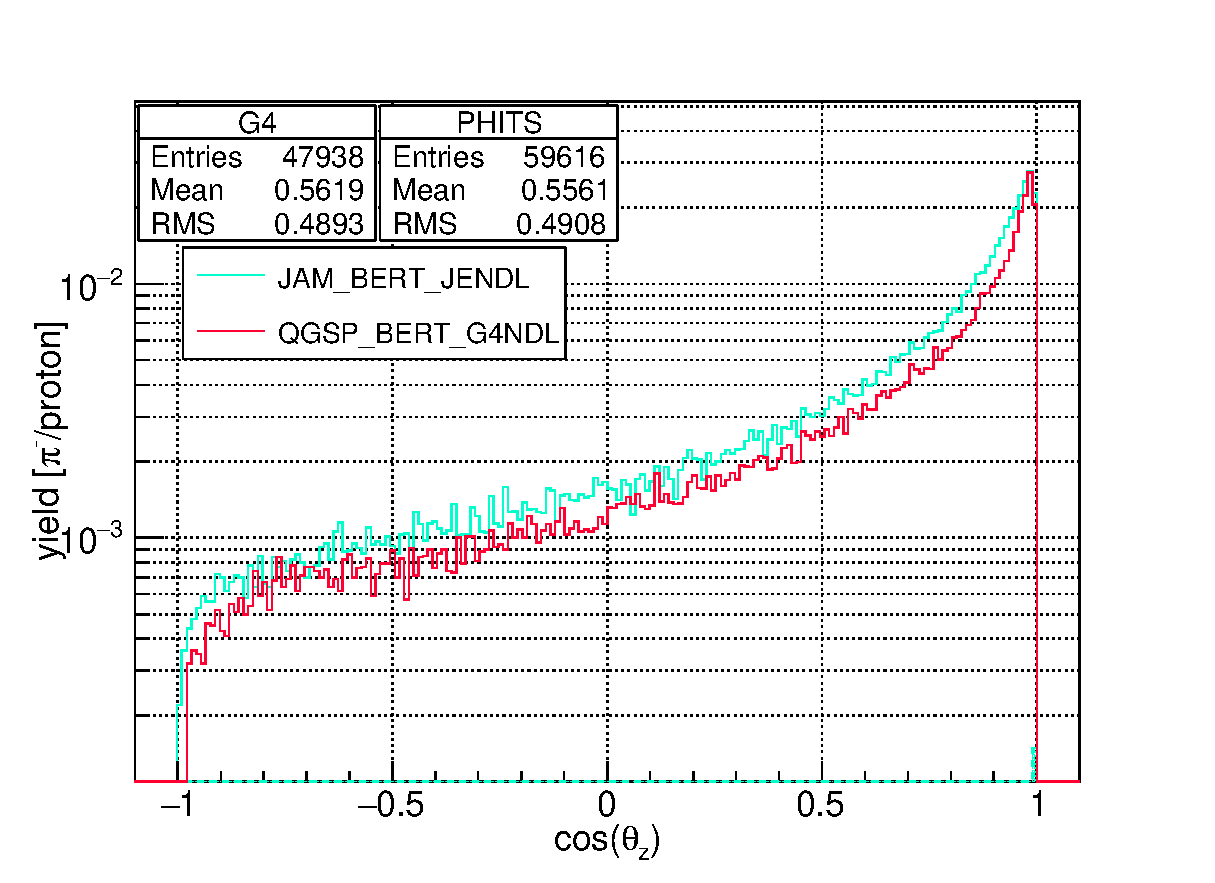
\includegraphics[scale=0.43]{chapter3/fig/backward.eps}
   \end{subfigure}
   \hspace{0.2\textwidth}
   \begin{subfigure}{0.3\textwidth}
    \centering
	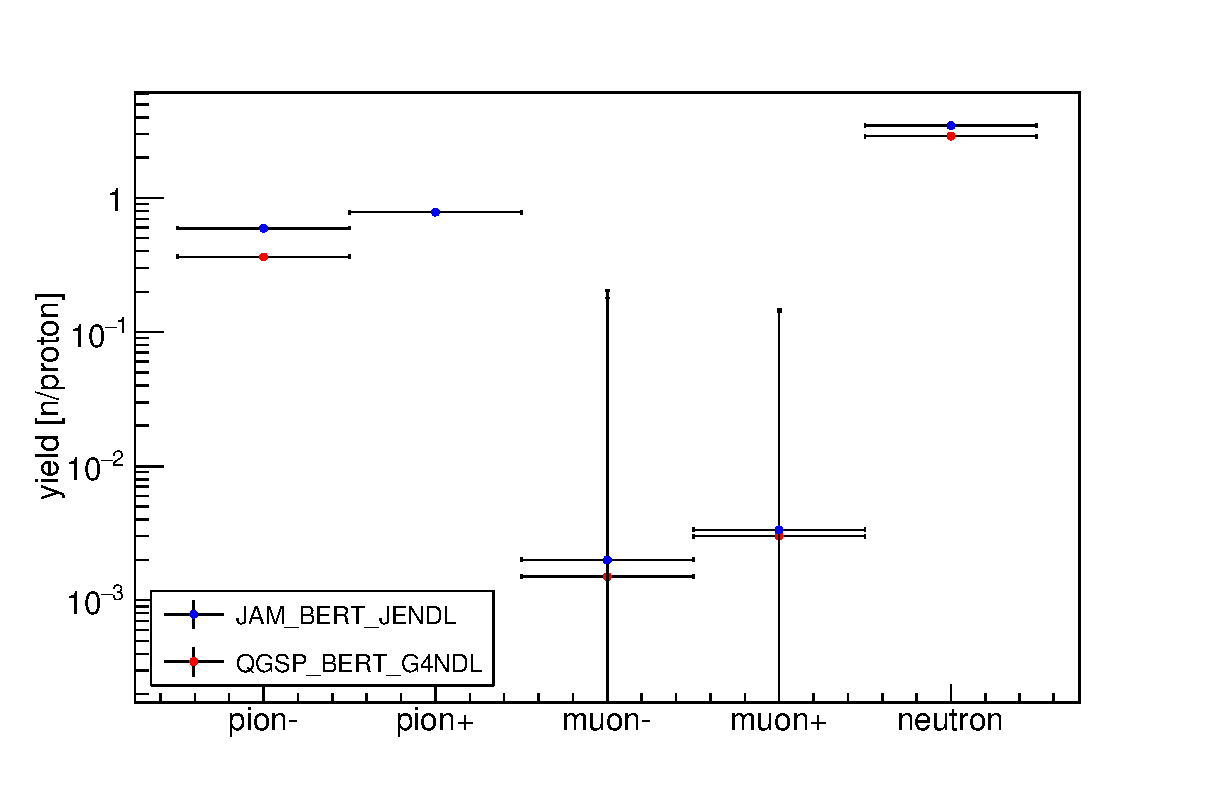
\includegraphics[scale=0.43]{chapter3/fig/production.eps}
   \end{subfigure}
   \caption{Compared the backward particle yield and integral yield with GEANT4 and PHITS. Left one is the backward pion and muon yield, red and blue line represent the yield calculated by QGSP\_BERT\_G4NDL and JAM\_BERT\_JENDL respectively. Right one shows the integral yield of pion and muon from target, red and blue point are the result of QGSP\_BERT\_G4NDL and JAM\_BERT\_JENDL.}
   \label{model}
  \end{figure}

  \subsection{Geometry}
~~~~~~The geometry plays an important role in radiation simulation, especially for the high energy physics.
Every detail of COMET phase-I geometry is established in PHITS simulation in terms of the design drawing from KEK.
 \begin{figure}[H]
   \centering
   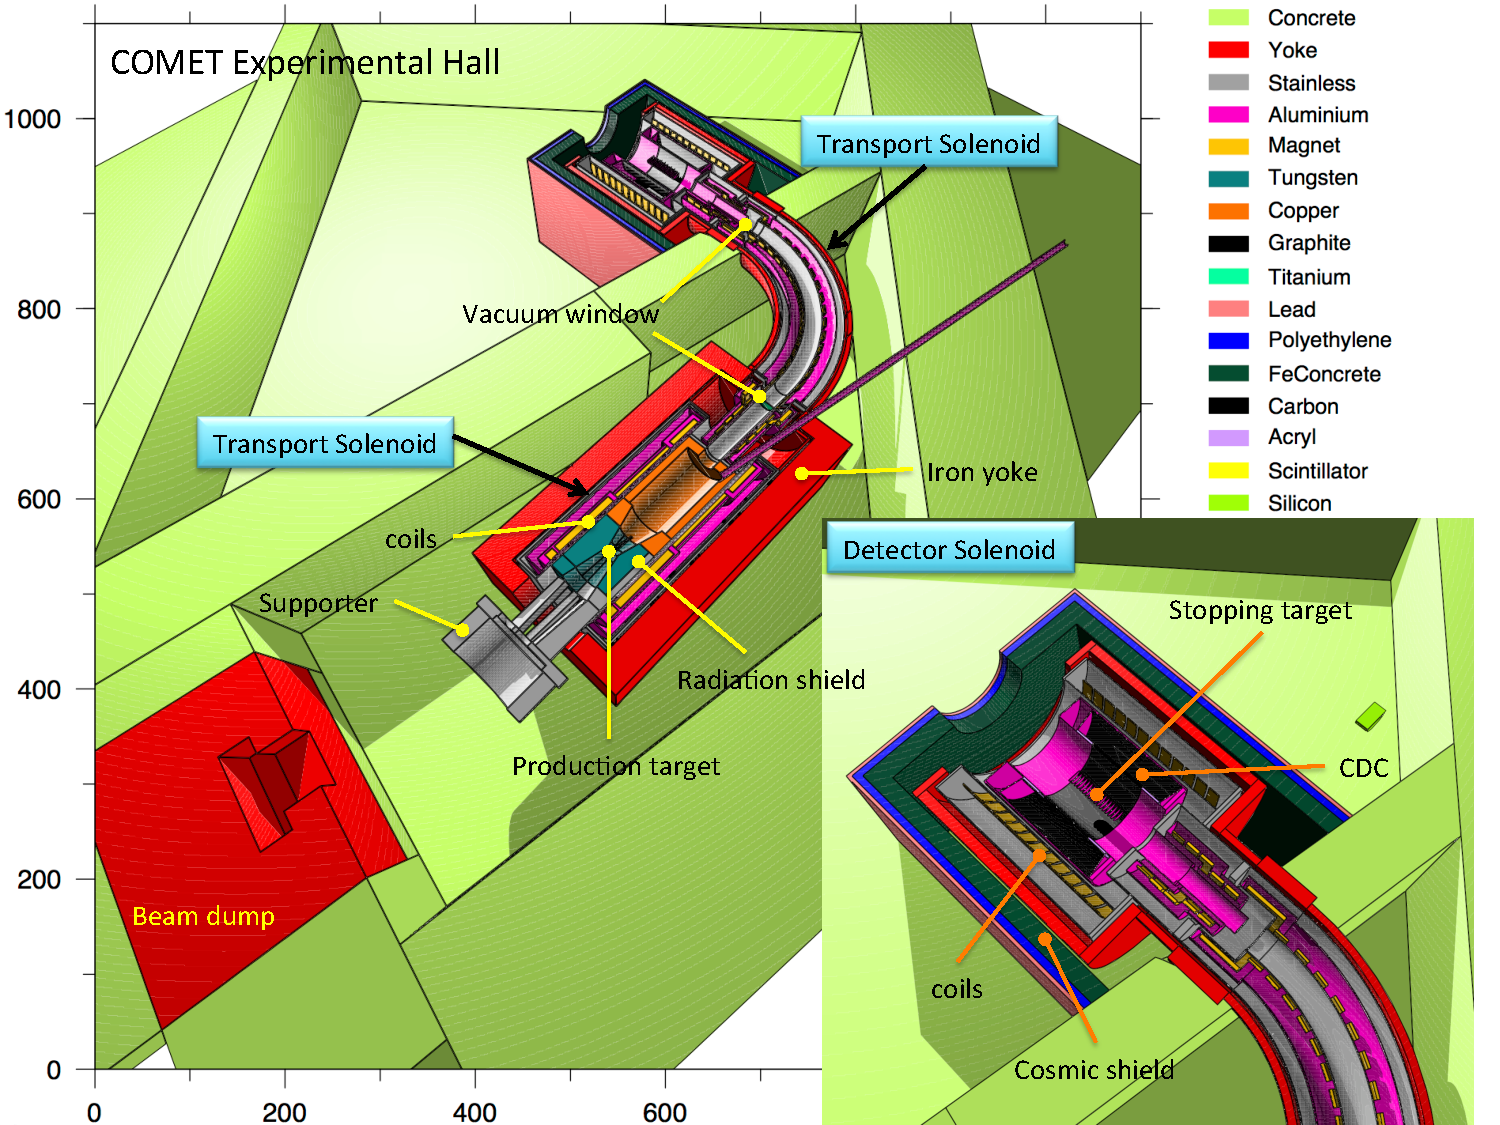
\includegraphics[scale=0.5]{chapter3/fig/geo.pdf}
   \caption{COMET phase-I experiment geometry in PHITS simulation.}
   \label{geom}
  \end{figure}
As shown in figure~\ref{geom}, the COMET experimental hall is seperated by concrete wall with 1 m thickness at end of 90 degree bending and 2 m at beam dump.
The concrete wall between experimental hall and control room and accelrator hall is with 3 m thickness to prevent the radiation leaking.
Beam dump consists of iron yoke with 1.5$\times$1.5$\times$1 m and 2.5$\times$2.5$\times$1 m holes which is same to the Mu2e beam absorber design and concrete~\cite{mu2ereport}.
Ceiling board is made of iron yoke with thickness of 0.6 m, gas (air) with thickness of 0.7 m and concrete with 3.7 m thickness.
Shielding supporter structure is made of stainless steel (SUS-304) with two holes for proton beam exit and target changing.
Radiation shield is employed the composit shield which will be described later.
In the muon beamline, two 1 mm titanium vacuum windows are set up in the end of pion capture solenoid and muon transport solenoid respectively.
Cosmic shield is consist of 20 cm concrete with 50\% iron, 10 cm polythylene and 10 cm lead.

  \subsection{Radiation estimation}
~~~~~~Since only backward pion is employed to create muon in high magnetic field, the main radiation is neutron and photon because they are not affected with magnetic field.
As implemented the geometry and magnetic field, the neutron and photon distribution is calculated and shown in figure~\ref{2photon}.
Because the geometry is only for phase-I experiment, the production target is replaced from graphite to pure tungsten target, and the proton beam intensity is changed to 4.4$\times$10$^{13}$ pps to estimate the radiation for phase-II experiment.
\begin{figure}[H]
   \begin{subfigure}{0.3\textwidth}
    \centering
    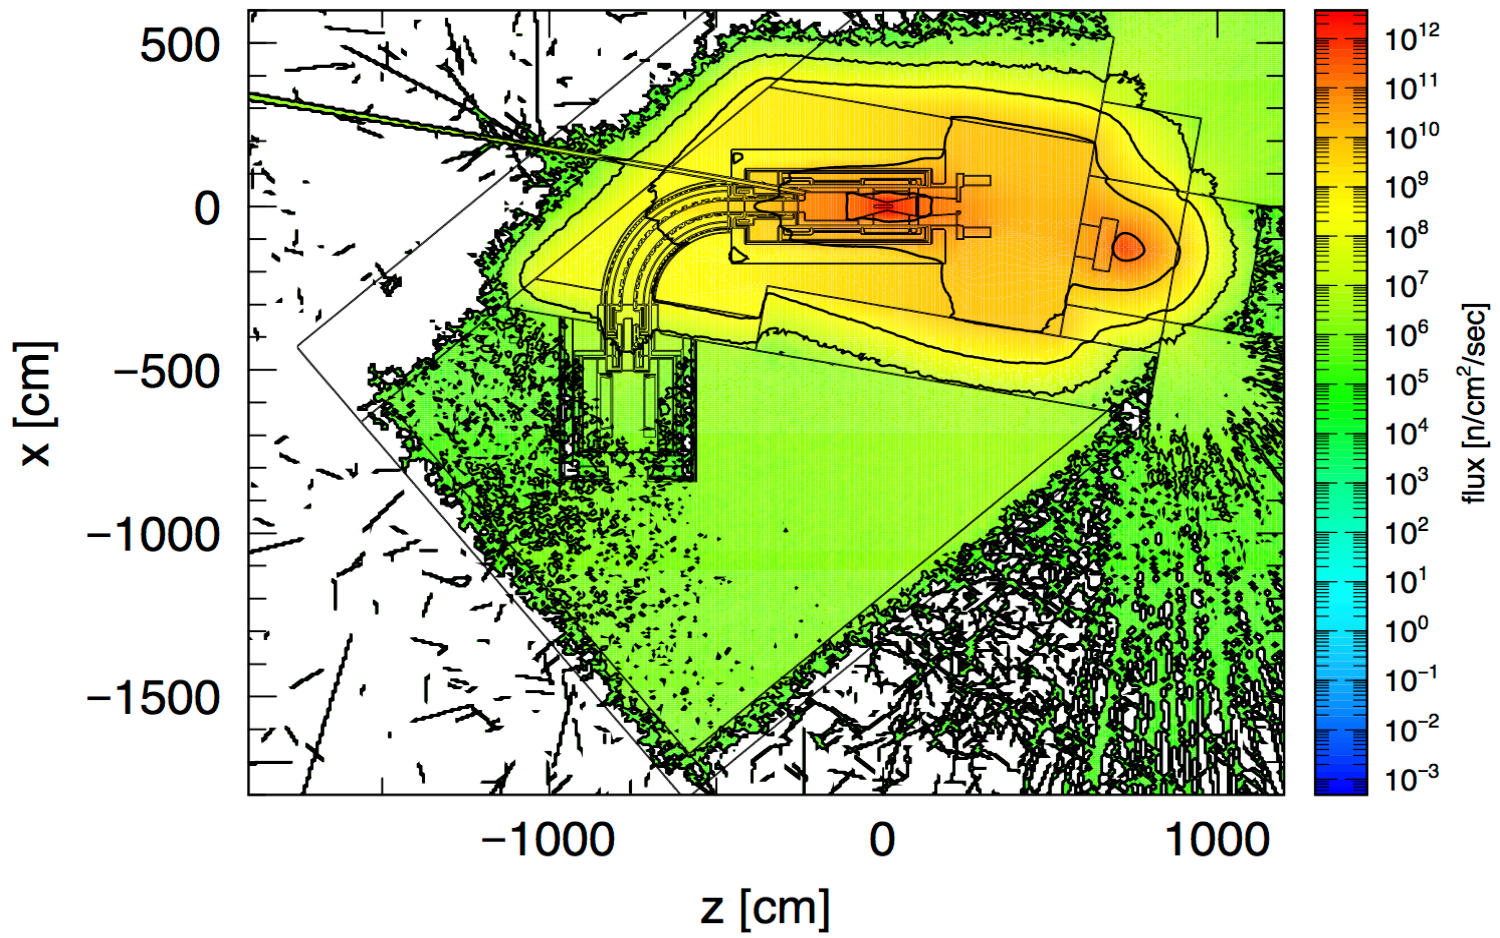
\includegraphics[scale=0.32]{chapter3/fig/neutronzx.pdf}
   \end{subfigure}
   \hspace{0.2\textwidth}
   \begin{subfigure}{0.3\textwidth}
    \centering
	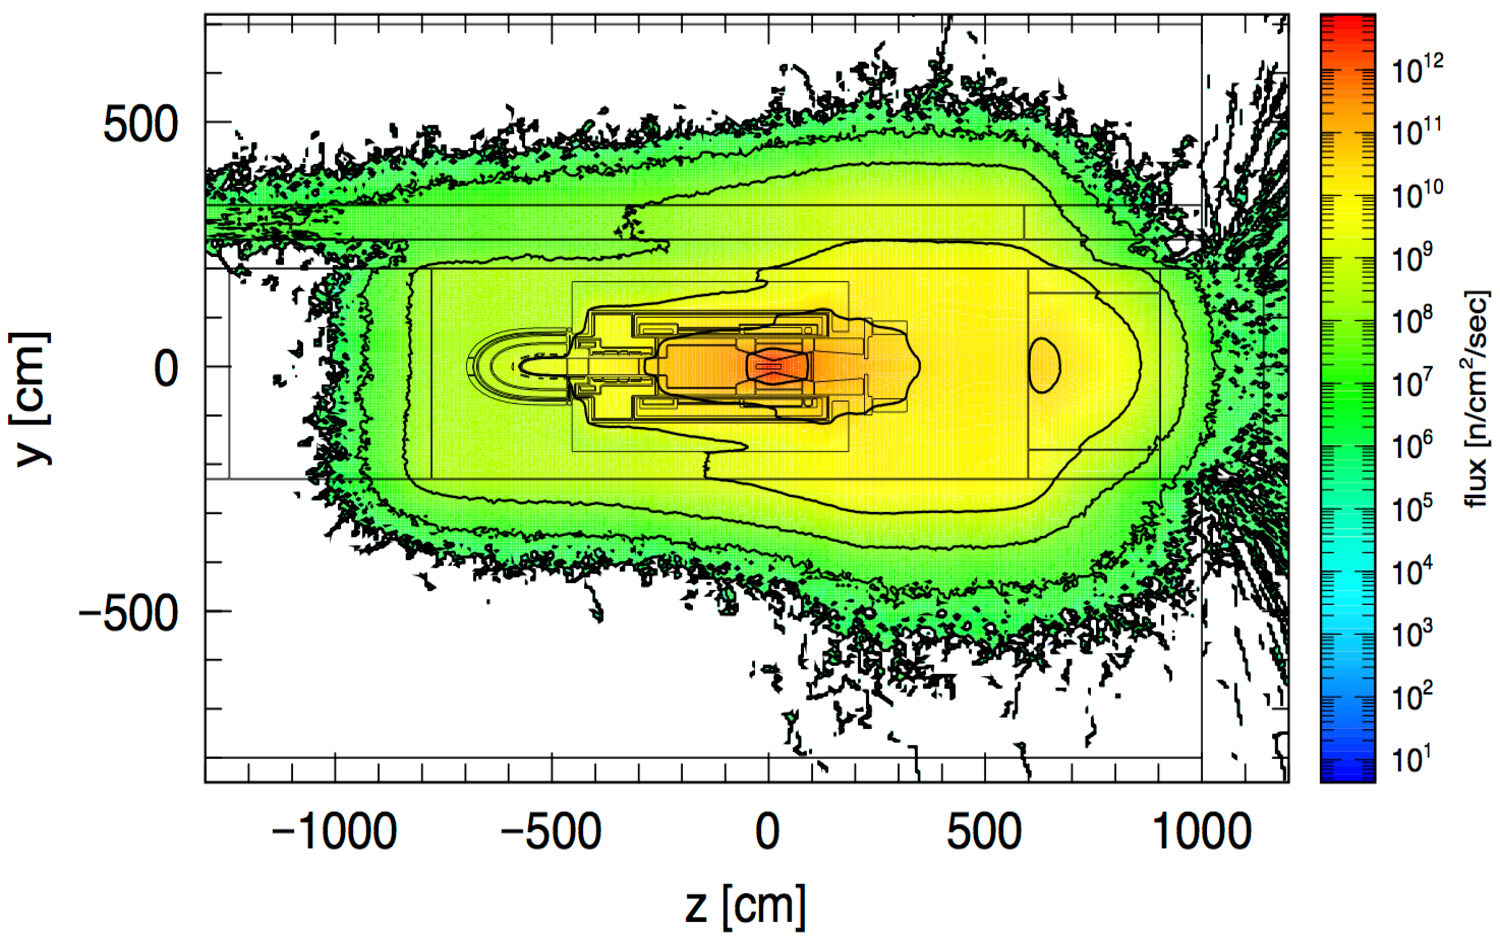
\includegraphics[scale=0.32]{chapter3/fig/neutronzy.pdf}
   \end{subfigure}
  % \caption{ The phase-II neutron distribution calculated with phase-II target and beam intensity.}
  % \label{neutrondist}
  \end{figure}
  \begin{figure}[H]
   \begin{subfigure}{0.26\textwidth}
   \centering
   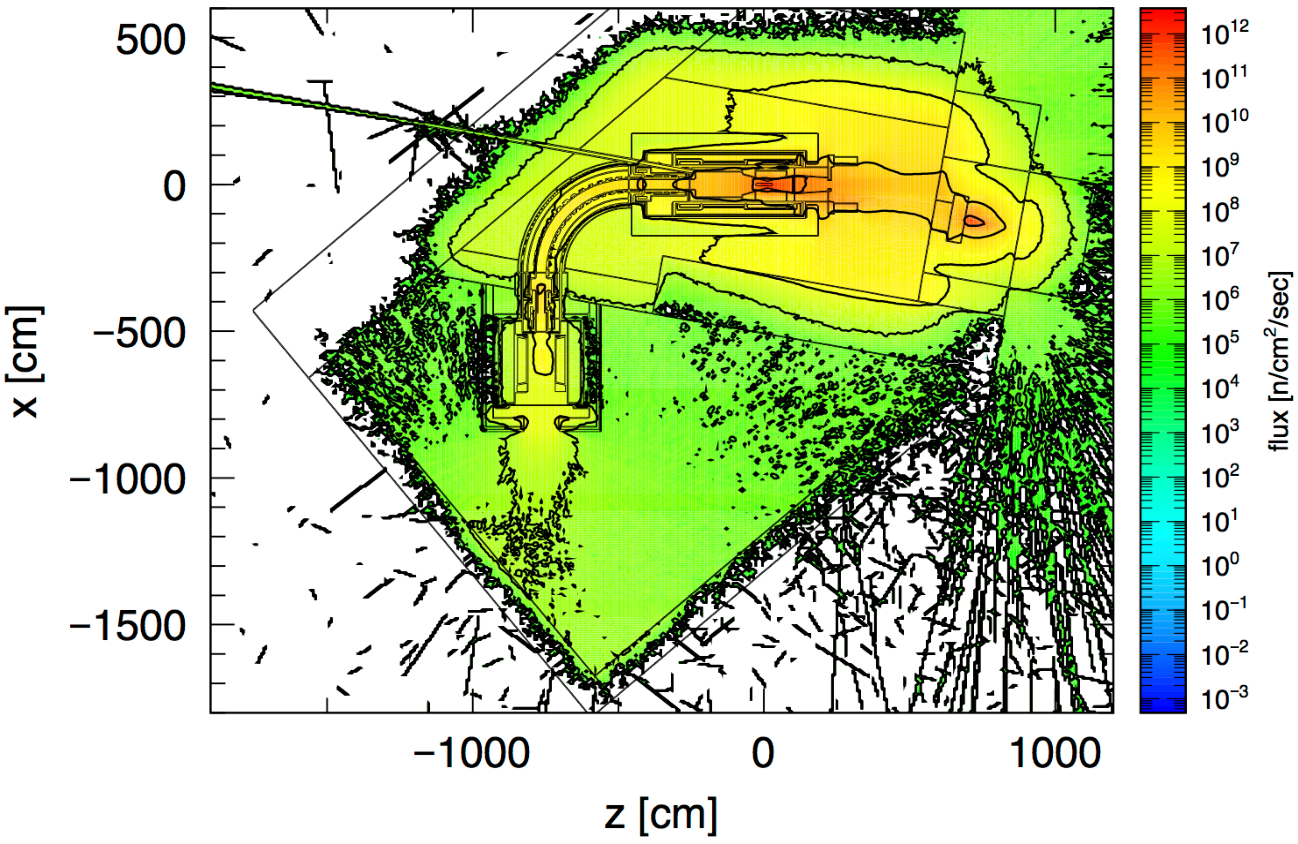
\includegraphics[scale=0.36]{chapter3/fig/photonzx.pdf}
   \end{subfigure}
   \hspace{0.2\textwidth}
   \begin{subfigure}{0.26\textwidth}
   \centering
   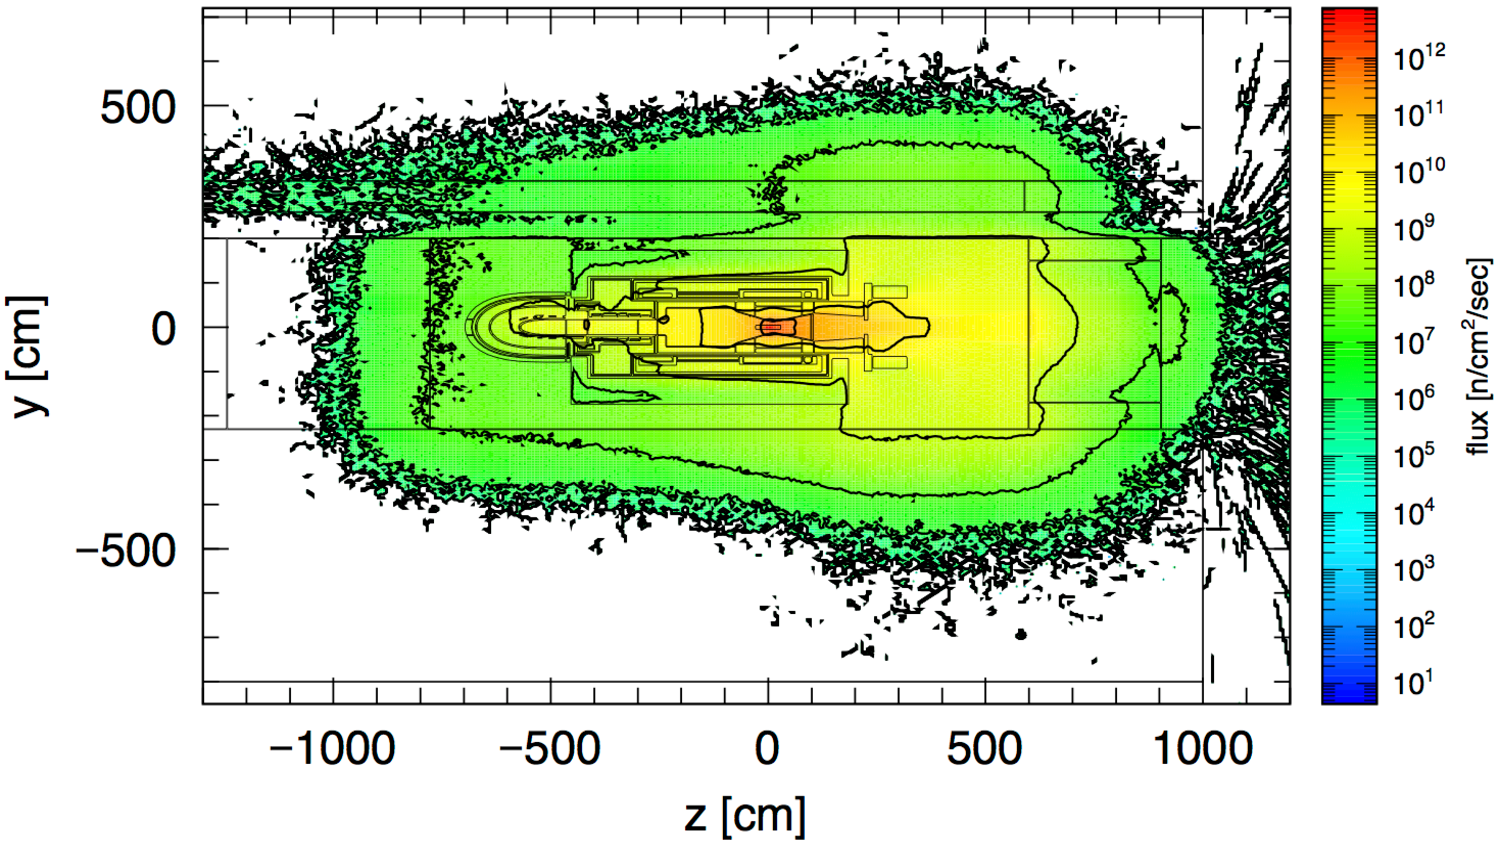
\includegraphics[scale=0.34]{chapter3/fig/photonyz.pdf}
   \end{subfigure}
   \caption{Neutron and photon distribution for COMET phase-II experiment. Top two show the neutron distribution from x-z and y-z view. Bottom two are the distribution of photon from x-z and y-z view.}
   \label{2photon}
  \end{figure}
Furthermore, to prevent neutrons leak to the detector room, the concrete wall with 2 m thick is replaced by iron yoke.
Even if the iron yoke is employed as a wall here, it still has 5$\times$10$^6$ n/cm$^2$/sec neutrons at least which leak from experimental room to detector room which is 5 times higher than phase-I exiperment.
The neutron along the muon beamline is with low energy and it is easy to be capture or scattered in the detector solenoid.
While, as for the photon, it comes from the neutron capture, muon capture, bremsstrahlung et al.
Thus, the photon in the detector solenoid is about 10$^9$ n/cm$^2$/sec at peak, which is 100 times higher than phase-I experiment at same place.

Figure~\ref{2bending} shows the energy spectrum of muon, photon and neutron for phase-II experiment at the end of 90 degree bending.
Compared with the other particle, neutron and photon is most dominated particle along the beamline.
Almost neutron is in the range of low energy, and photon is with energy from 0.01 MeV to 100 MeV.
  \begin{figure}[H]
   \centering
   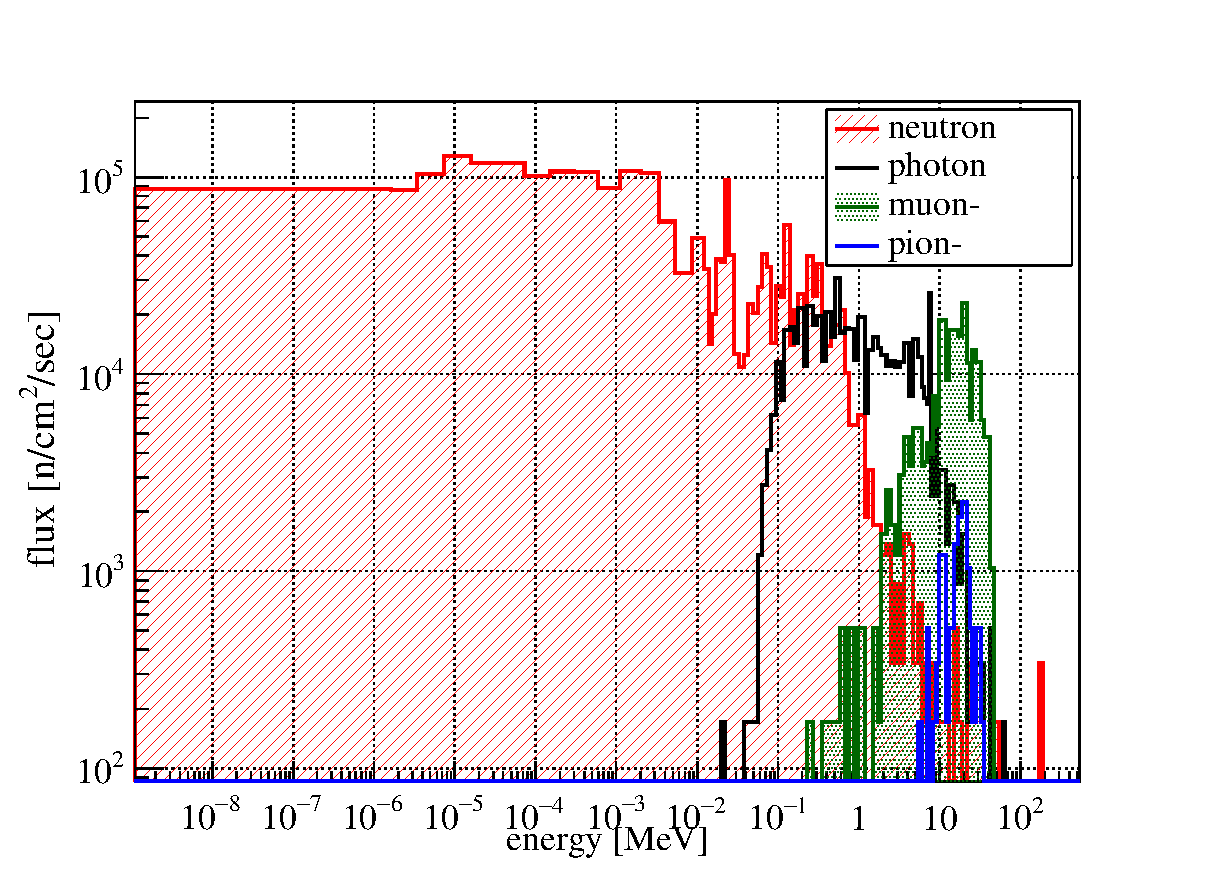
\includegraphics[scale=0.43]{chapter3/fig/Neutron.eps}
   \caption{Energy spectrum of muon, photon and neutron from both experimental hall and beamline at the end of 90 degree bending. Most of neutrons are at the low energy region, and photon are all higher than 10 keV.}
   \label{2bending}
  \end{figure}
  \begin{figure}[H]
   \centering
   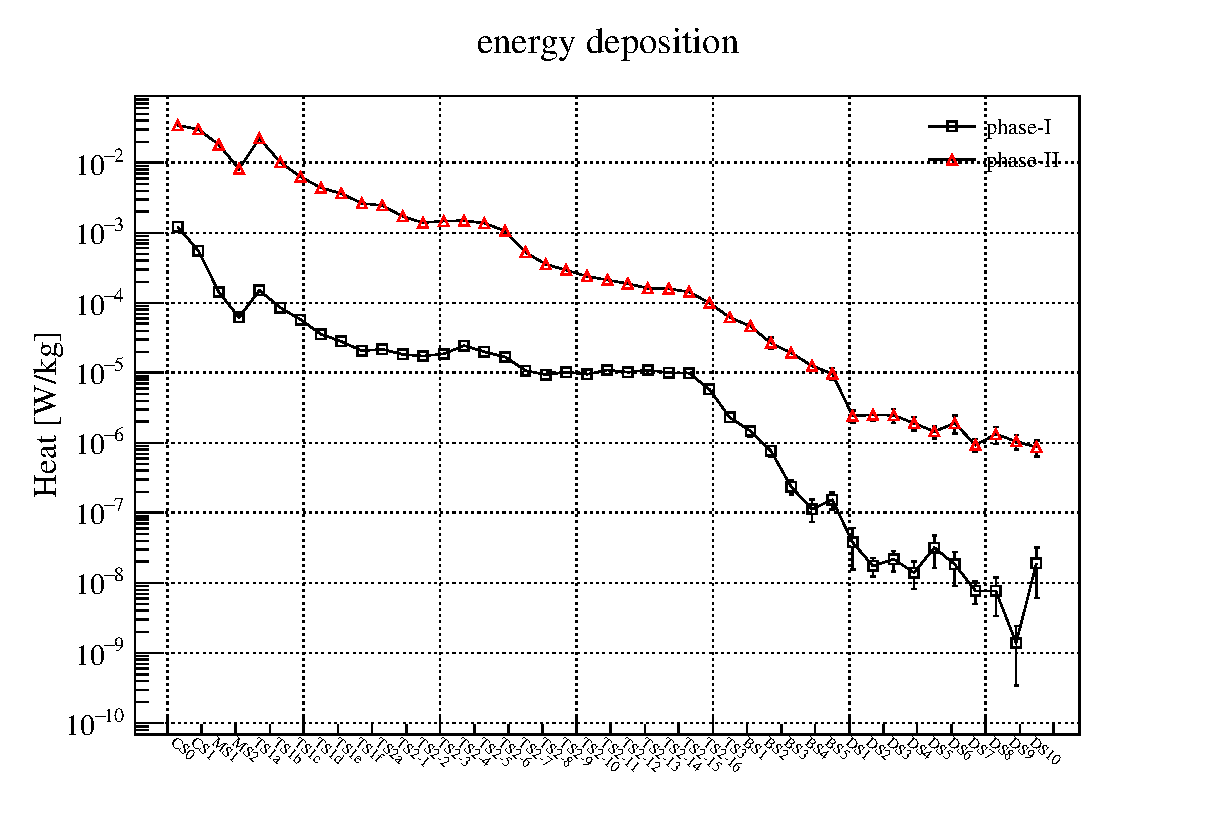
\includegraphics[scale=0.43]{chapter3/fig/heat.eps}
   \caption{The energy deposition of each magnets in phase-I and phase-II experiment. Black and red point represent the energy deposition of phase-I and phase-II experiment respectively. The energy deposition of phase-II is one order higher than phase-I's, and its peak is located in CS0 coil.}
   \label{2heat}
  \end{figure}
The radiation remains thier energy into superconducting coils, which will cause the hot spot inside the magnets.
Once the hot spot is generated in the superconducting magnet, these magnets are at risk from quench.
The heat load of each magnet for phase-I and phase-II experiment are shown in figure~\ref{2heat}.
Compared with phase-I experiment, heat load of phase-II experiment is 10 times higher than phase-I experiment at least.
The peak of heat load is at CS0 coil which 0.03 W/kg correspending to 0.73 MGy for 280-day operation.

 \section{Residual radiation estimation}
~~~~~~To achieve the muon with higher intensity, the graphite target will be replaced by pure tungten target after phase-I experiment finished.
Thus, the residual radiation plays an important role in target changing and maintainance of the superconducting magnets.
The residual radiation has been investigated by using FLUKA code and PHITS code.

%  \subsection{Cross section comparison}
%~~~~~~In order to ensure the calculation of residual radiation, the activation cross section in PHITS code has been compared with the experimental data.
%Considering that COMET experiment is using the 8 GeV proton beam, which covers the INCL and JAM physical model in PHITS, the selection of the experimental data must be higher than 3.5 GeV.
%The activation cross section at high energy region has been compared with the experimental data from JASMIN collaboration~\cite{jasmin}.
%As the comparison shown in figure~\ref{yashima}, PHITS code has good agreement with the experimental data.
%\begin{figure}[H]
% \begin{subfigure}{0.3\textwidth}
%  \centering
%  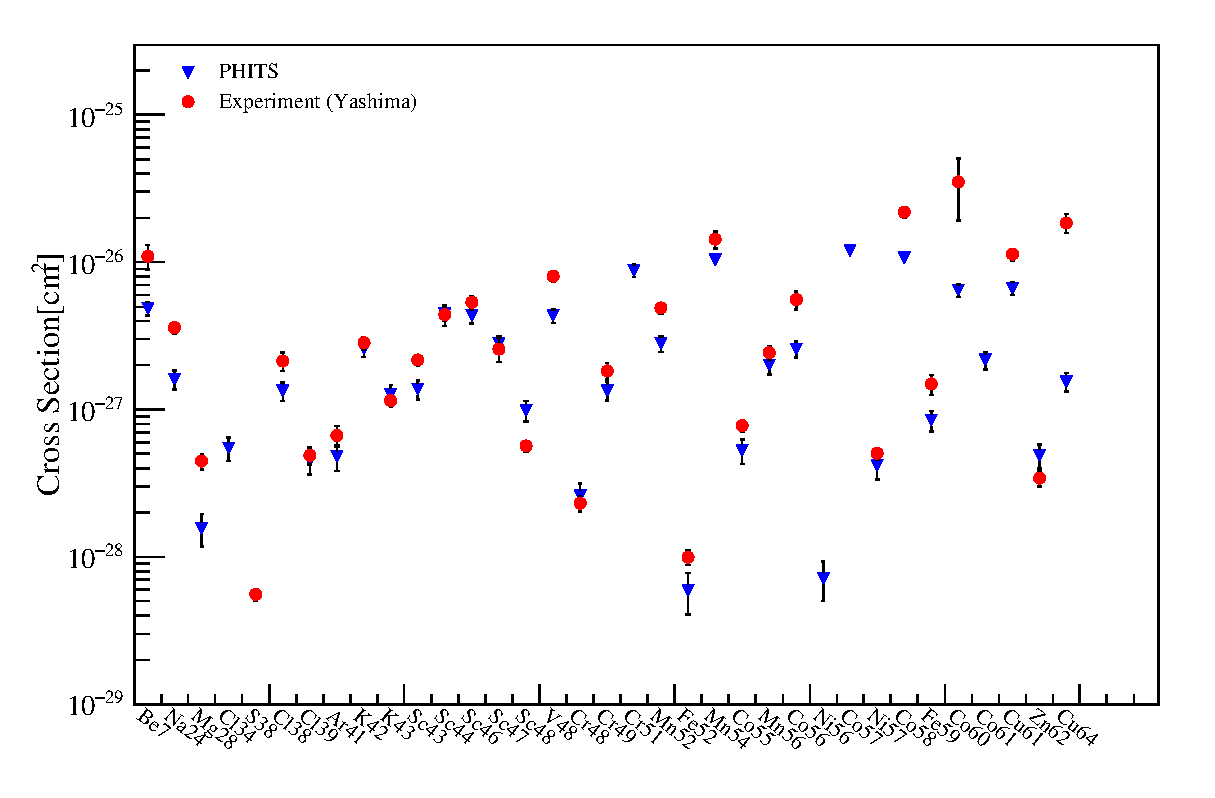
\includegraphics[scale=0.43]{chapter3/fig/copper}
  %\caption{ Copper}
  %\label{fig:cuyashima}
%  \end{subfigure}
%  \hspace{0.2\textwidth}
% \begin{subfigure}{0.3\textwidth}
%  \centering
%  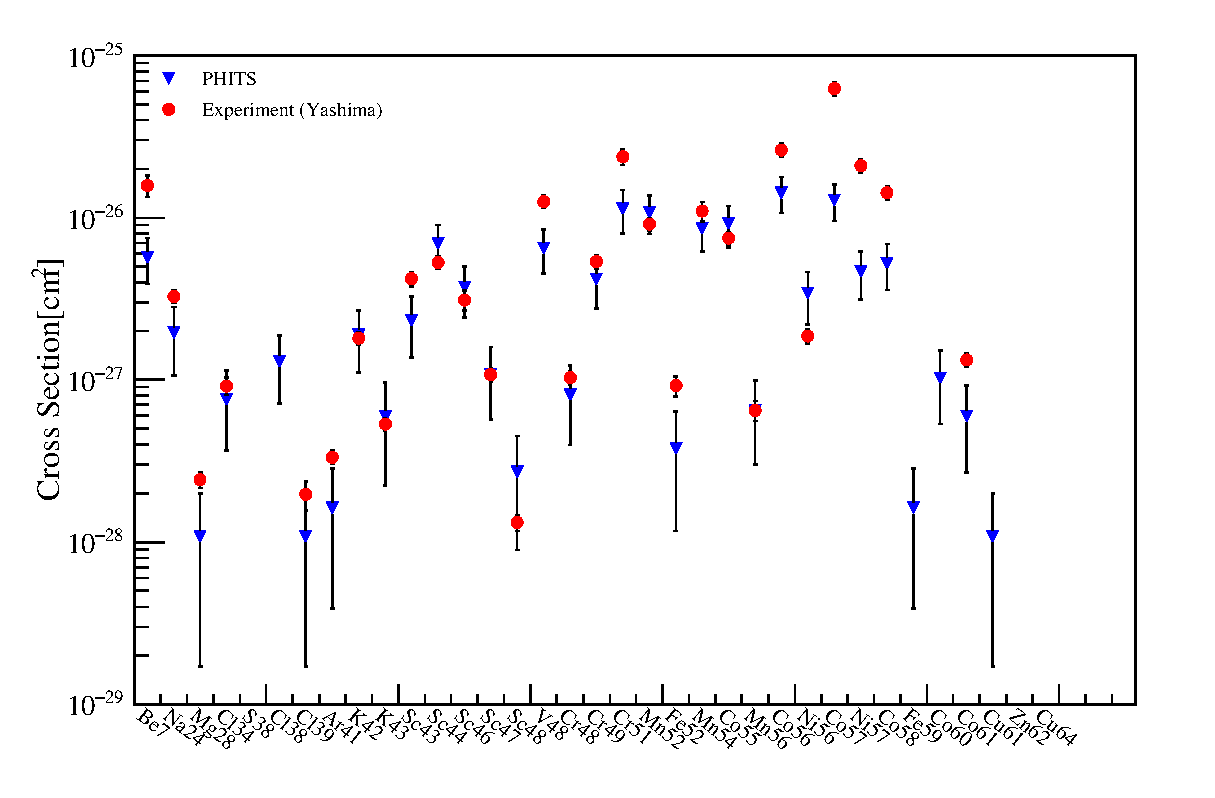
\includegraphics[scale=0.43]{chapter3/fig/nickel}
  %\caption{ Nickel}
  %\label{fig:coyashima}
%  \end{subfigure}
%  \caption{Comparison of the activation cross section from experiment with PHTIS. Figure on left and right show the activation cross section of copper and nickel. The activation cross section is measured in FermiLAB by HPGe detector, using 120 GeV, 1.0$\times$10$^9$ pps roton beam.}
%  \label{yashima}
%\end{figure}

  \subsection{Residual radiation}
~~~~~~The residual radiation of each part of solenoid is estimated by PHITS and DCHAIN-SP code~\cite{dchain}.
DCHAIN-SP code is a dedicated software for the residual radiation developed by JAEA.
Using the result of nucleus yield from PHITS code, the photon flux and its intensity is able to be calculated by DCHAIN-SP.
Then, the distribution of residual radiation is estimated by
\begin{equation}
 E(\epsilon) = f(\epsilon) \cdot \phi(\epsilon)
\end{equation}
where $E(\epsilon)$ and $\phi(\epsilon)$ are the effective dose and the gamma ray flux calculated in DCHAIN-SP.
The fluence-to-effective dose conversion coefficients $f(\epsilon)$ is shown in reference~\cite{flco} with unit of Sv/cm$^2$.

The operation time schedule used in calculation are 1-year cooling after 1-month running with intensity of 2.5$\times$10$^{12}$ pps, which are all base on the phase-I experiment.
Residual radiation of vacuum vessel, magnet, radiation shield and iron yoke are given by figure~\ref{2part}.
To reduce the residual radiation as much as possible, considering copper is hard to weld with stainless steel, some parts of vacuum vessel is able to be changed to iron.
As listed in table~\ref{vecuum}, residual radiation of stainless steel is 10 times higher than iron's.
Thus, the stainless steel is replaced by iron for vacuum vessel outside the superconducting magnet due to magnetism of iron.
 \begin{figure}[H]
  \centering
  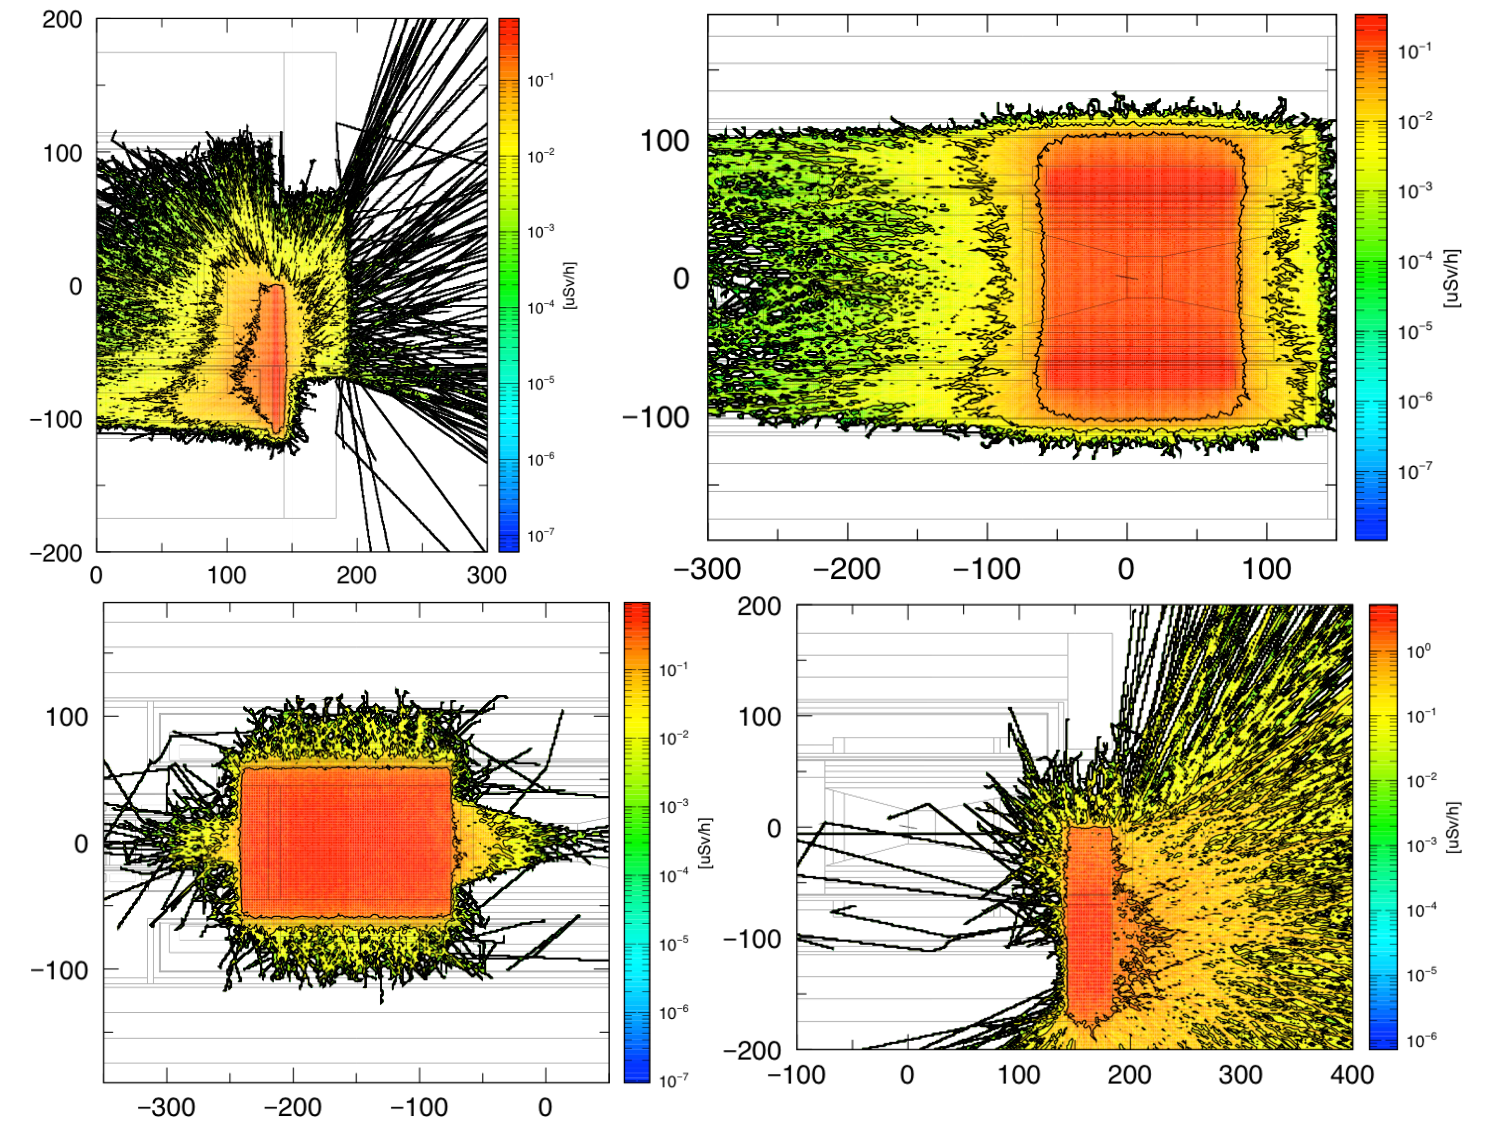
\includegraphics[scale=0.43]{chapter3/fig/partres.pdf}
  \caption{Residual radiation of vacuum vessel, magnet, radiation shield and iron yoke with 1 month operation and 10 month cooling.}
  \label{2part}
 \end{figure}
\begin{table}[H]
 \centering
 \begin{tabular}{ccc} \hline \hline
  & Stainless steel & Iron  \\ \hline
  Radiation dose [$\mu$Sv/h] & 7.00 & 0.65 \\ \hline \hline
 \end{tabular}
 \caption{Residual radiation of vacuum vessel between CS0 and iron yoke.}
 \label{vecuum}
\end{table}

The residual radiation of superconducting magnet is calculated as one conductor which consists of aluminum, copper and NbTi with density of 4.0 g/cm$^3$.
The activity and radiation dose given by figure~\ref{2dose} shows that the maximum radiation dose is 0.33 $\mu$Sv/h after 1 month operation and 10 month cooling for phase-I experiment and the peak of activation is at CS0 and CS1.
Isotopes like $^{93}$Nb, $^{22}$Na, $^3$H, $^{60}$Co et al. with long half life are generated in CS1 and CS0 coils.
 \begin{figure}[H]
  \begin{subfigure}{0.3\textwidth}
   \centering
   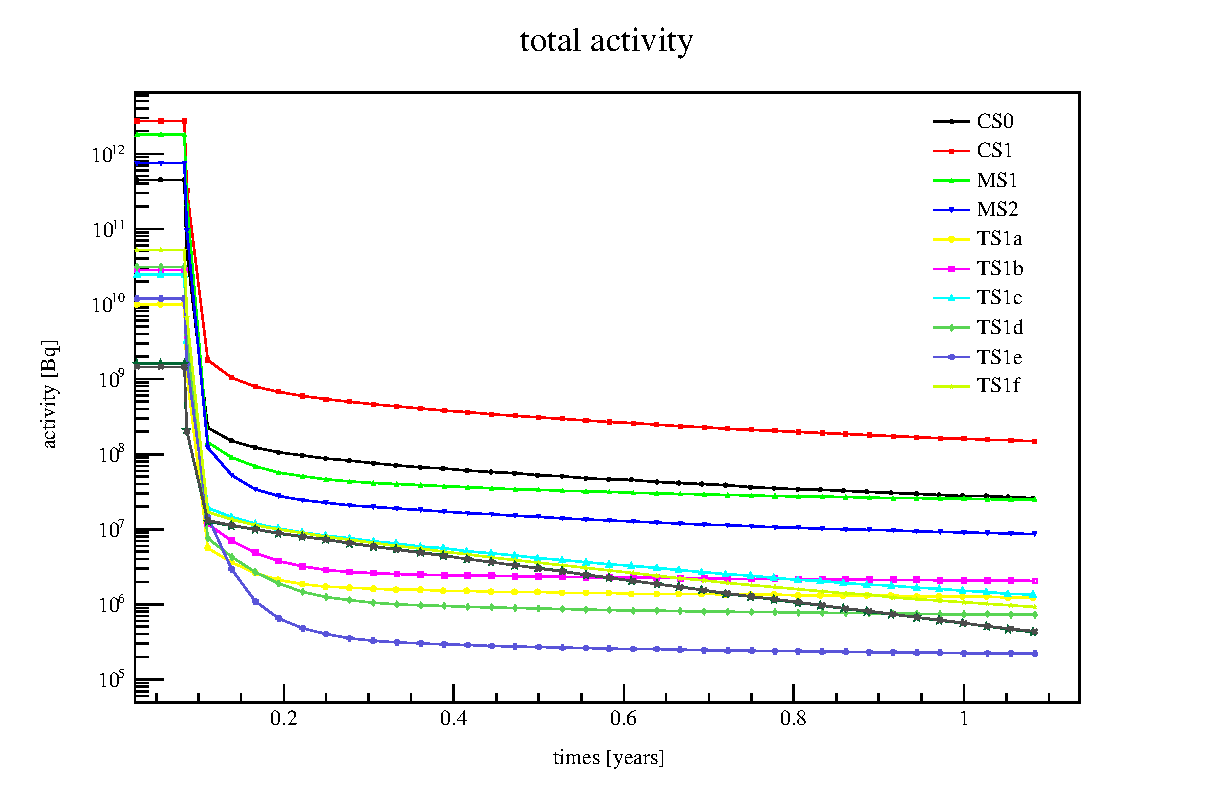
\includegraphics[scale=0.45]{chapter3/fig/activity.eps}
  \end{subfigure}
  \hspace{0.2\textwidth}
  \begin{subfigure}{0.3\textwidth}
   \centering
   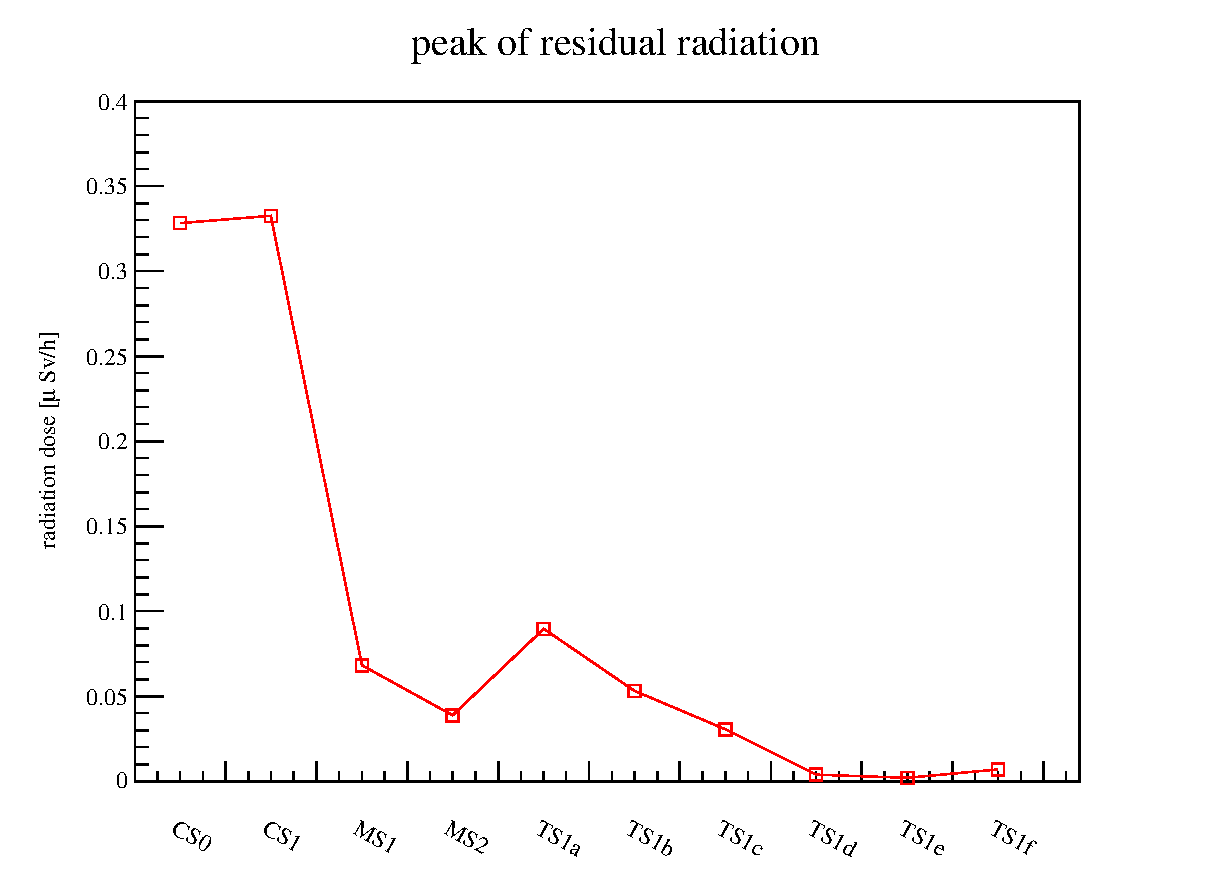
\includegraphics[scale=0.40]{chapter3/fig/dose.eps}
  \end{subfigure}
  \caption{Activity and peak of dose equivalent of each magnets with 1-month operation and 10-month cooling.}
  \label{2dose}
 \end{figure}

Because PHITS and DCHAIN-SP only can calculate the residual radiation from a defined region, it may cause the average of the radiation if the geometry is cut to many tiny meshes.
Figure~\ref{2dose2} (left) shows the total dose equivalent predicted by PHITS and DCHAIN-SP.
It is added from many parts of small regions.
The maximum dose equivalent is predicted to 0.75 mSv/h for 1-month operation and 10-month cooling at production target.
To ensure the dose equivalent, we also compare this result with FLUKA code which can simulate the residual radiation dose without region cutting.
M. Brugger et al. present the residual radiation calculated from FLUKA code has good agreement experimental data~\cite{brugger}.
 \begin{figure}[H]
  \begin{subfigure}{0.3\textwidth}
   \centering
   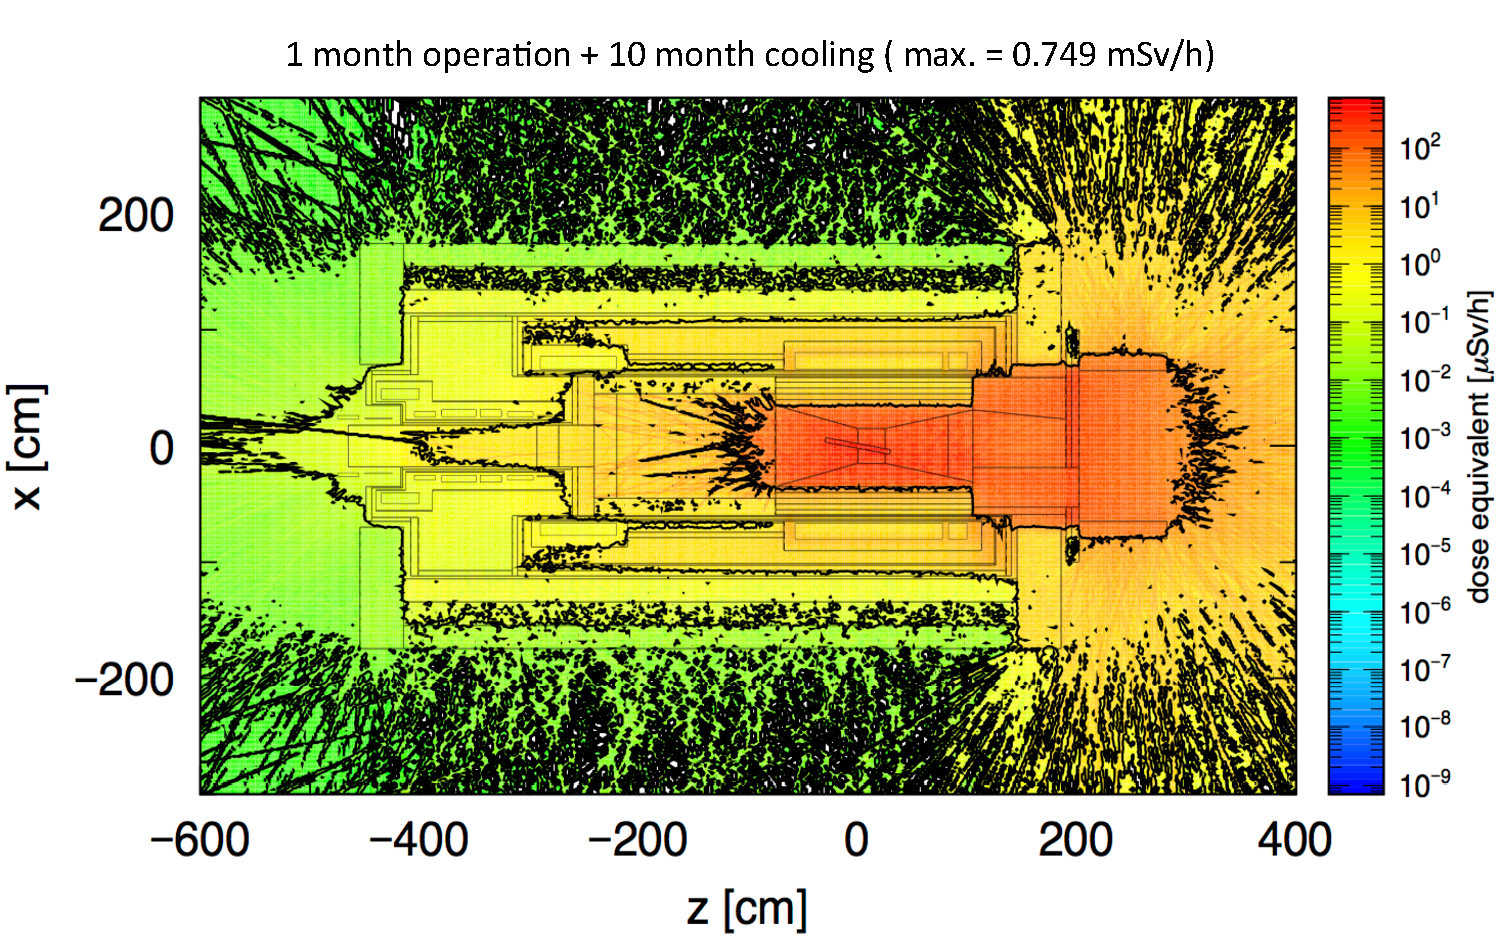
\includegraphics[scale=0.33]{chapter3/fig/phitsdose.pdf}
  \end{subfigure}
  \hspace{0.2\textwidth}
  \begin{subfigure}{0.3\textwidth}
   \centering
   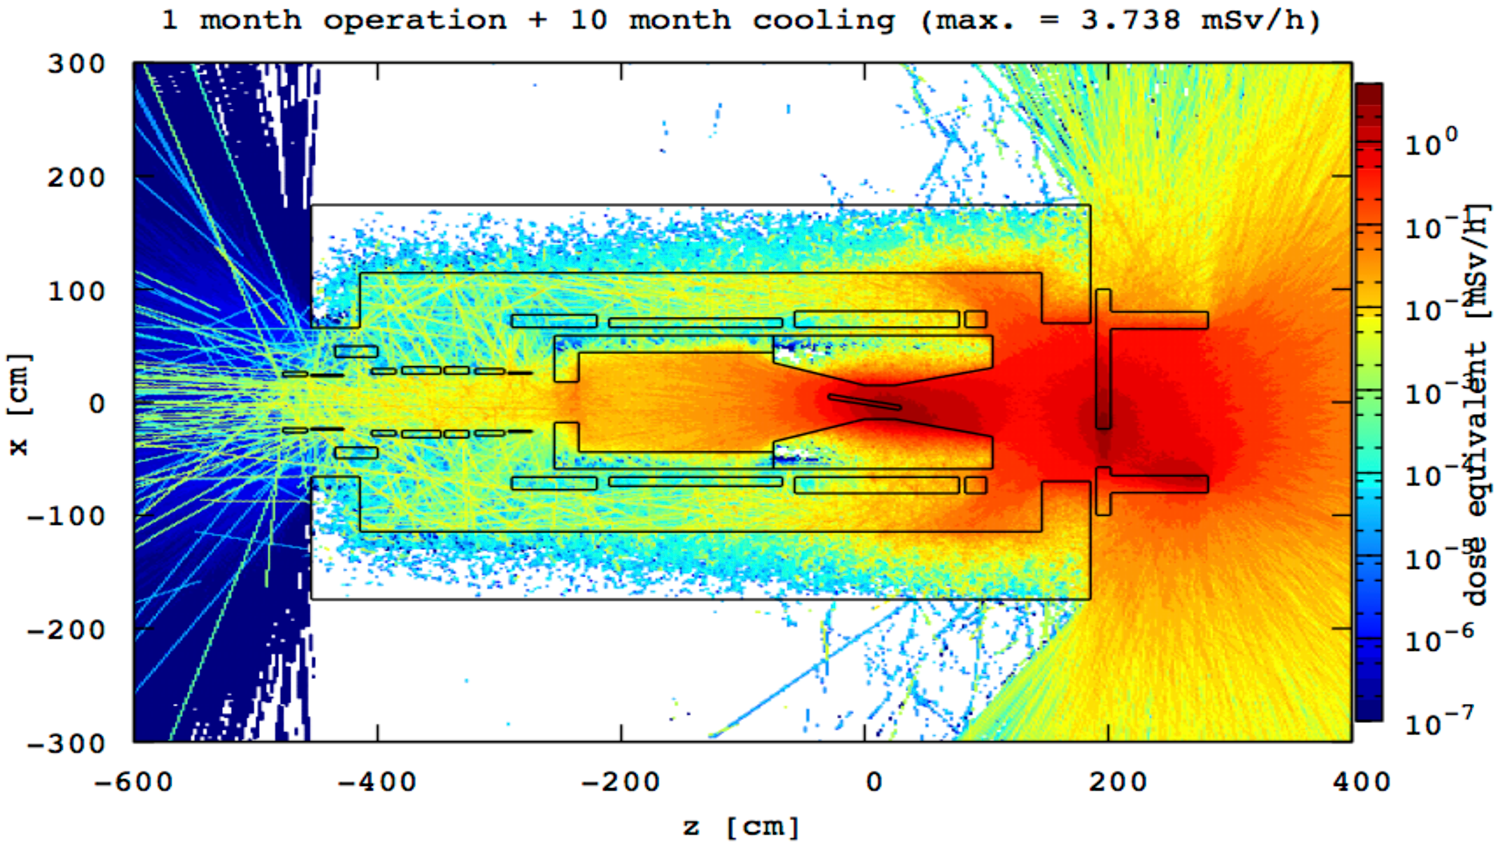
\includegraphics[scale=0.33]{chapter3/fig/flukadose.pdf}
  \end{subfigure}
  \caption{Compared the residual radiation distribution of pion capture solenoid between PHITS and FLUKA. Left and right represent the PHITS and FLUKA result respectively.}
  \label{2dose2}
 \end{figure}
As the result shown in figure~\ref{2dose2} (right), the maximum dose equivalent is predicted to 3.74 mSv/h with same time schedule, which is 5 times higher than PHITS result.
In figure~\ref{dosepo}, the dose equivalent at different position along the axis is compared.
Besides the place where peak is, the dose equivalent is quite similar between the FLUKA and PHITS.
Difference may be owing to the mesh cutting of PHITS calculation around target.
 \begin{table}[H]
 \centering
 \begin{tabular}{ccccc} \hline \hline
  Code & z = 0 & z = 300 & z = -300 & z = -500 \\
   & [mSv/h] & [mSv/h] & [mSv/h] & [mSv/h] \\ \hline
  FLUKA & 3.74 & 0.04 & 0.009 & 0.002 \\
  PHITS & 0.75 & 0.03 & 0.01 & 0.002 \\ \hline \hline
 \end{tabular}
 \caption{Compared the residual radiation along the z axis. z=0 is at the production target, z=-300 is 3 m far from the target on upstream of target, z=300 is 3 m far from the target on dreamstream of target, and z=-500 is 5 m far from teh target.}
 \label{dosepo}
\end{table}
Because of the target changing after phase-I experiment, this residual radiation is still too high for co-workers.
Table~\ref{2time} gives the maximum residual radiation after cooling for 10 months, 1.75 year and 2 years.
\begin{table}[H]
 \centering
 \begin{tabular}{cc} \hline \hline
  Time [year] & Maximum residual radiation [mSv/h] \\ \hline
  0.83 & 3.738 \\
  1.75 & 1.125 \\
  2.00 & 1.013 \\ \hline \hline
 \end{tabular}
 \caption{Maximum residual radiation after cooling for 10 months, 1.75 year and 2 years.}
 \label{2time}
\end{table}
From this estimation, the residual radiation will be reduced about 3 times after cooling for 2 years compared with 10 month cooling.
Considering the beam dump is not included into this simulation, working for 1 hour is possible for co-workers.

 \section{Radiation shielding optimization}
~~~~~~The heat and radiation shield (HRS) is located around the production target to protect the superconducting from the radiation exposure.
This radiation shield consists of two parts, one is for protecting MS magnets, another one is for protecting CS magnets.
It is unable to take long time to change the radiation shield after phase-I experiment due to the residual radiation.
Thus, radiation shield must be designed for both phase-I and phase-II experiment.

Pure tungsten is most ideal material as the radiation shield due to its high density.
However, it has several disadvantages such as high costs, heavy mass and complex fabrication.
Therefore, some parts of radiation shield can be replaced by the other materials.

 \subsection{Radiation shield for MS}
~~~~~~Inside the superconducting magnets, radiation shield must be made of material without magnetism.
Thus, there are two candidates for MS radiation shield, copper and stainless steel.
The heat load of each CS and MS magnet when the copper and stainless steel is used as radiation is estimated by PHITS code in table~\ref{hrsload}.
It shows that copper shield has better shielding ability than stainless steel shield.
 \begin{table}[H]
 \centering
 \begin{tabular}{cccccc} \hline \hline
  & CS0 [W] & CS1 [W] & MS1 [W] & MS2 [W] & CS + MS [W] \\ \hline
  SUS304 & 8.03 & 51.82 & 27.80 & 10.49 & 98.13 \\
  Copper & 7.56 & 50.14 & 22.99 & 8.73 & 89.42 \\ \hline \hline
 \end{tabular}
 \caption{Heat load of stainless steel and copper shield.}
 \label{hrsload}
\end{table}
Considering the residual radiation of radiation shield, the actived isotopes and activity after 1-month operation and 10-month cooling are investigated and shown in table~\ref{2atom}.
Apparently, copper shield's activity is quite lower than stainless steel shield's.
Furthermore, the dose equivalent of copper and stainless steel shield are 1.51 $\mu$Sv/h and 7.02 $\mu$Sv/h respectively.

From the aspect of shielding ability and residual radiation, copper is the better material for MS radiation shield.
Noting that the induced current will be generated by the changing of magnetic field, the copper should be cut in somewhere.
\begin{table}[H]
 \centering
 \begin{tabular}{c}
  \begin{minipage}{0.4\textwidth}
  \centering
  \begin{tabular}{ccc} \hline \hline
   Nuclei & Activity [MBq] & Half life [year] \\ \hline
   $^{60}$Co & 192 & 5.27 \\
   $^{57}$Co & 111 & 0.75 \\
   $^{63}$Ni & 80.9 & 100 \\
   $^{58}$Co & 56.9 & 0.19 \\
   $^{54}$Mn & 54.7 & 0.86 \\
   $^3$H & 30.9 & 12.3 \\
   $^{55}$Fe & 29.3 & 2.73 \\
   $^{49}$V & 16.7 & 0.90 \\
   $^{56}$Co & 5.52 & 0.21 \\
   $^{65}$Zn & 5.13 & 0.67 \\ \hline \hline
  \end{tabular}
  %\caption{Actived isotopes of copper shield.}
  \end{minipage}
  \hspace{0.1\textwidth}
  \begin{minipage}{0.4\textwidth}
  \centering
  \begin{tabular}{ccc} \hline \hline
   Nuclei & Activity [MBq] & Half life [year] \\ \hline
   $^{55}$Fe & 4950 & 2.73 \\
   $^{54}$Mn & 1500 & 0.86 \\
   $^{49}$V & 878 & 0.90 \\
   $^{57}$Co & 585 & 0.75 \\
   $^{58}$Co & 387 & 0.19 \\
   $^{51}$Cr & 92.6 & 0.08 \\
   $^{59}$Fe & 29.4 & 0.12 \\
   $^{63}$Ni & 26.5 & 100 \\
   $^3$H & 26.0 & 12.3 \\
   $^{60}$Co & 21.7 & 5.27 \\ \hline \hline
  \end{tabular}
  %\caption{Actived isotopes of stainless steel shield.}
  \end{minipage}
 \end{tabular}
 \caption{Actived isotopes of copper (left) and stainless steel (right).}
 \label{2atom}
\end{table}

\subsection{Radiation shield for CS}
~~~~~~Proton is injected into pion capture solenoid with 10 degree, thus, a hot spot is created on the one side of CS1 and CS0 coils, which is the one of the reason why quench occurs.
Thus, the radiation shield for CS requires
\begin{itemize}
 \setlength{\itemsep}{-5pt}
 \item Limit the maximum heat load in coils.
 \item Limit the maximum radiation induced damage in coils.
 \item Reduce the mass of radiation shield.
 \item Pion yield should not be reduced significantly.
\end{itemize}

To eliminate the hot spot and keep the balance, the low radiation region which corresponds to the side far to incident proton enables to be fabricated by another kind of material.
As for the material, the ideal material is pure tungsten but only the tungsten alloy is cheaper and easy to fabricate.
Thus, the details of tungsten alloy (AN-1800) are list in table~\ref{alloy}.
 \begin{figure}[H]
  \begin{subfigure}{0.3\textwidth}
   \centering
   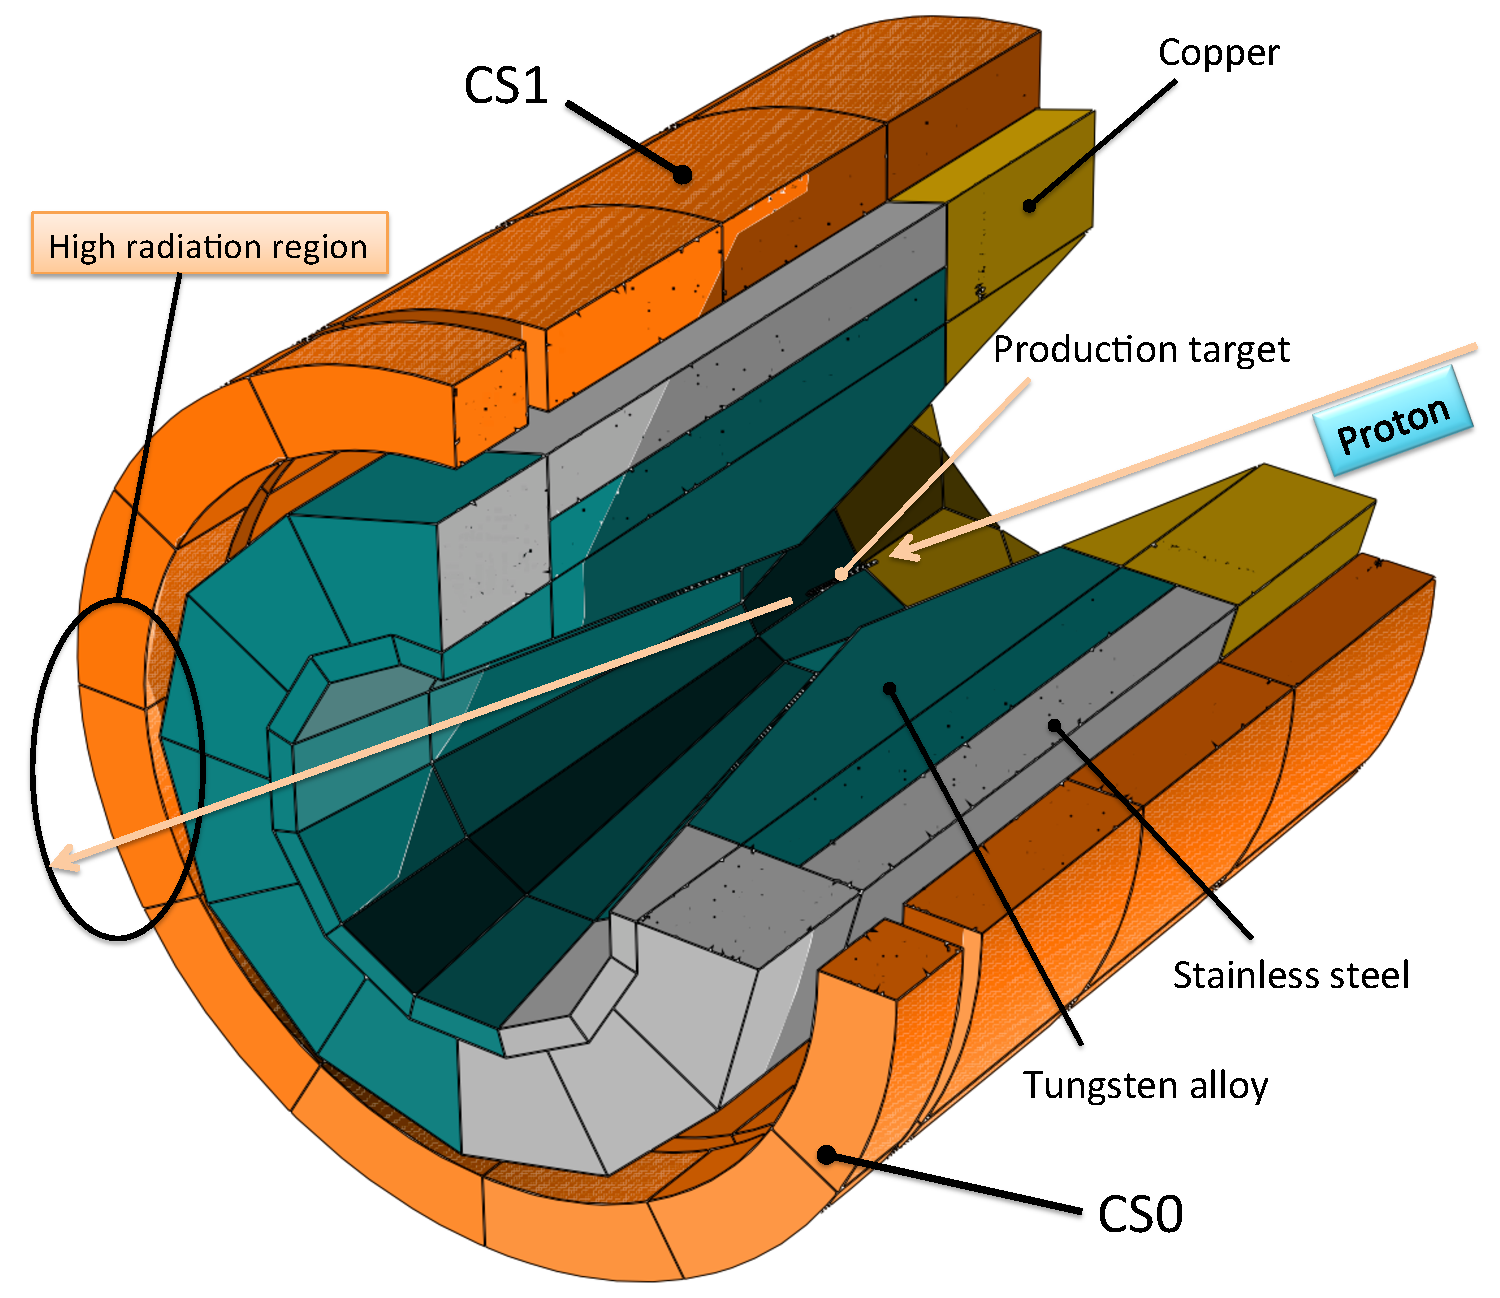
\includegraphics[scale=0.3]{chapter3/fig/shielding.pdf}
  \end{subfigure}
  \hspace{0.2\textwidth}
  \begin{subfigure}{0.3\textwidth}
   \centering
   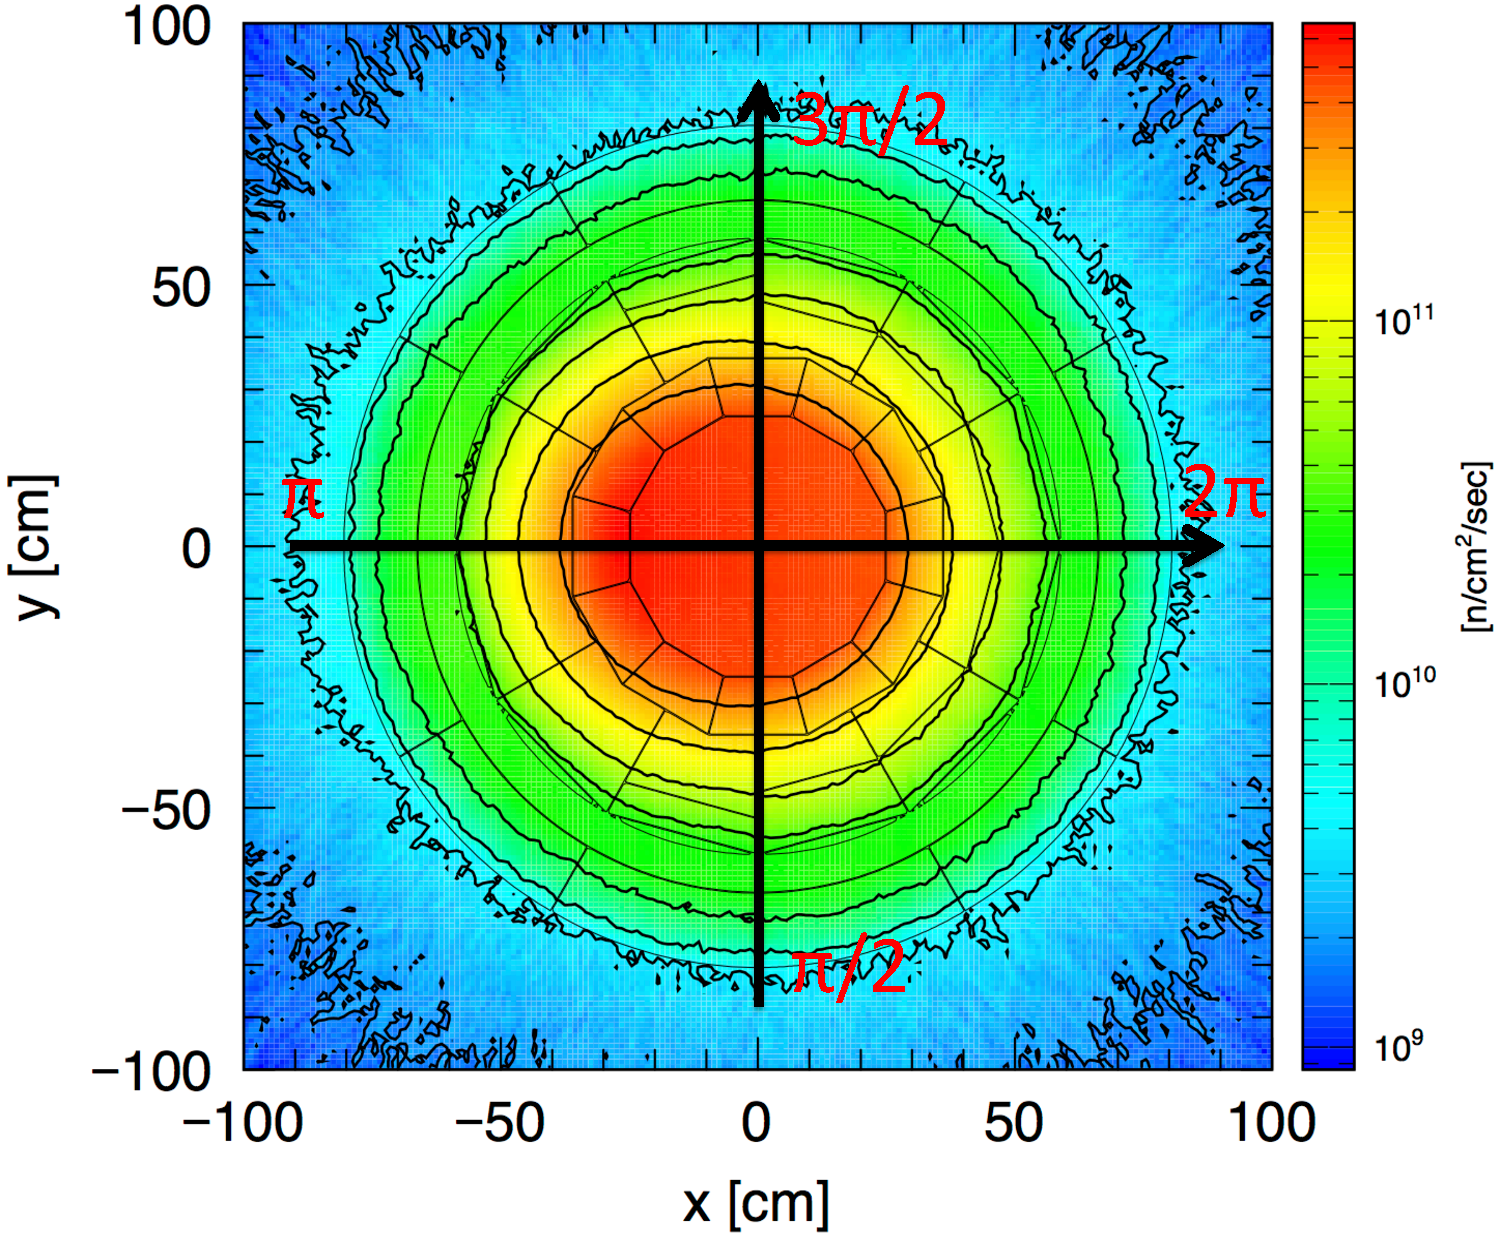
\includegraphics[scale=0.3]{chapter3/fig/shieldflux.pdf}
  \end{subfigure}
  \caption{The concept of COMET radiation shield. It consists of tungsten alloy, stainless steel and copper. Tungsten ally and stainless steel are employed on the high and low radiation side respectively. On the downstream of target, copper is used. Right figure shows the distribution of neutron from x-y view. Azimuthal angle is also defined in here. The peak of neutron flux is located at 180 degree of CS coils.}
  \label{2shieldgeo}
 \end{figure}
\begin{table}[H]
 \centering
 \begin{tabular}{cc} \hline \hline
  Composition [wt.\%] & Ni: 3.0$_{\pm 0.25}$; Cu: 2.0$_{\pm 0.25}$; W: 95.0$_{\pm 0.5}$ \\
  Density [g/cm$^3$] & 18.0$_{\pm 0.2}$ \\
  Hardness & HV 320$_{\pm 50}$ \\
  Tensile strength & 620 MPa \\
  Offset yield strength & 500 MPa \\
  Elastic modulus & 310 GPa \\
  Thermal conductivity & 104 W/m/K \\
  Thermal expansion coefficient & 5.5$\times$10$^{-6}$ K$^{-1}$ \\ \hline \hline
%  Shielding ability & 47\% ($^{60}$Co radiation source) \\
 \end{tabular}
 \caption{Material property of tungsten alloy (AN-1800).}
 \label{alloy}
\end{table}
As shown in figure~\ref{2shieldgeo}, the radiation shield is designed which consists of tungsten alloy, copper and stainless steel.
The DPA, neutron fluence and heat load of several shielding design concepts along azimuthal direction is compared in figure~\ref{2dpa} and \ref{2flux}.
Details of several shielding designs are listed as follows.
 \begin{figure}[H]
  \begin{subfigure}{0.3\textwidth}
   \centering
   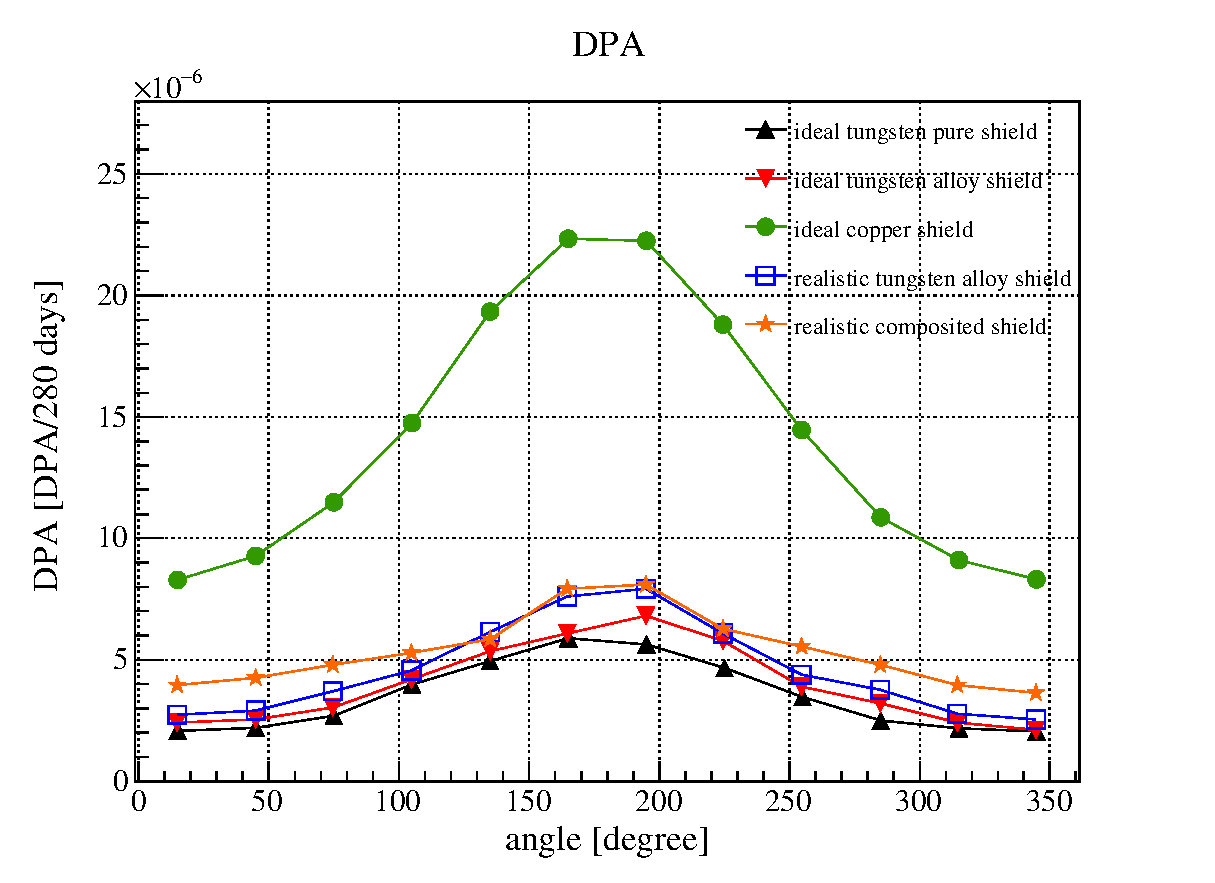
\includegraphics[scale=0.43]{chapter3/fig/dpa.eps}
  \end{subfigure}
  \hspace{0.2\textwidth}
  \begin{subfigure}{0.3\textwidth}
   \centering
   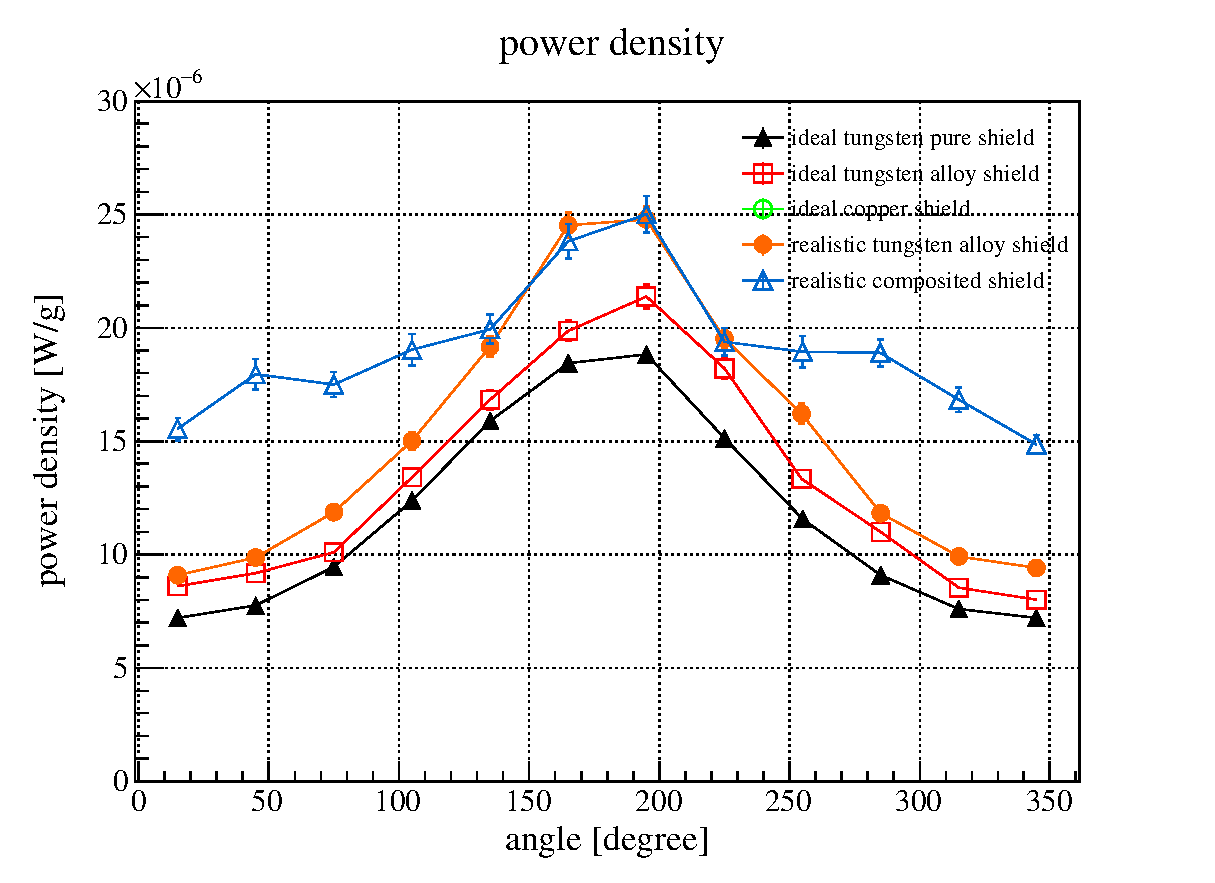
\includegraphics[scale=0.43]{chapter3/fig/shieldheat.eps}
  \end{subfigure}
  \caption{Compared the azimuthal DPA and energy deposition of middel part of CS1 coil in different verion of shielding design. The long CS1 coil is cut to 3 parts along the z axis and 12 parts along the azimuthal axis.}
  \label{2dpa}
 \end{figure}
\begin{itemize}
 \setlength{\itemsep}{-5pt}
 \item Ideal pure tungsten shield: made of pure tungsten with a cylindrical shape.
 \item Ideal tungsten alloy shield: made of tungsten alloy with a cylindrical shape.
 \item Ideal copper shield: made of copper with a cylindrical shape.
 \item Realistic tungsten alloy shield: made of tungsten alloy with a polygonal shape.
 \item Realistic composited shield: made of tungsten alloy, copper and stainless steel with a polygonal shape.
\end{itemize}

After these comparisons, we come out the conclusion
\begin{itemize}
 \setlength{\itemsep}{-5pt}
 \item The maximum DPA of CS1 coils increases over 4 times when the pure tungsten is replaced by copper.
 \item Compared with tungsten alloy, pure tungsten has stronger shielding ability.
 \item Shielding ability of cylindrical shape is stronger than polygonal shape.
 \item The peak of DPA, heat load and neutron fluence is same between composited shield and tungsten alloy shield.
\end{itemize}
The details of shielding design is listed in table~\ref{hrsdet}.
 \begin{figure}[H]
  \centering
  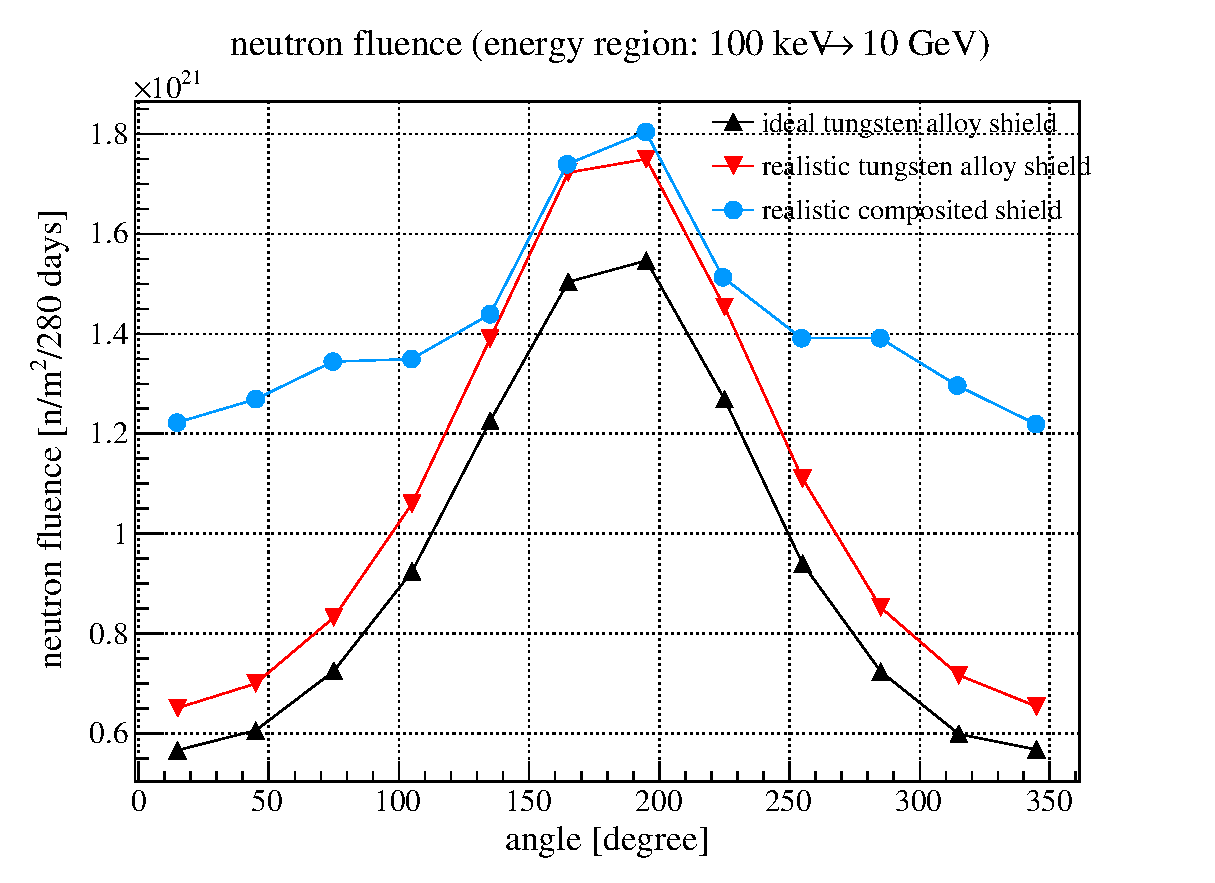
\includegraphics[scale=0.43]{chapter3/fig/fluence}
  \caption{High energy neutron (E $\geq$ 0.1 MeV) along the azimuthal direction of CS1 coils.}
  \label{2flux}
 \end{figure}
\begin{table}[H]
 \centering
 \begin{tabular}{ccc} \hline \hline
  CS1 & Composited shield & Pure tungsten shield \\ \hline
  peak neutron fluence [n/m$^2$/280 days] & 2.35$\times$10$^{21}$ & 2.26$\times$10$^{21}$ \\
  peak power density [W/g] & 2.50$\times$10$^{-5}$ & 2.40$\times$10$^{-5}$ \\
  power [W] & 57.5 & 36.6 \\
  peak dose [MGy/280 days] & 0.79 & 0.76 \\
  peak DPA [DPA/280 days] & 1.05$\times$10$^{-5}$ & 0.98$\times$10$^{-5}$ \\
  tungsten mass [t] & 15.6 & 28 \\ \hline \hline
 \end{tabular}
 \caption{Details of the shielding design. CS1 is cut to 3 parts along the z axis, 12 parts along the azimuthal direction.}
 \label{hrsdet}
\end{table}

As for the muon yield, it does not depend on the material of radiation but the backward radius of shield.
Figure~\ref{radius} shows that the muon and pion yield increases about 9\% after the radius is changed from 36 cm to 50 cm.
\begin{figure}[H]
 \centering
 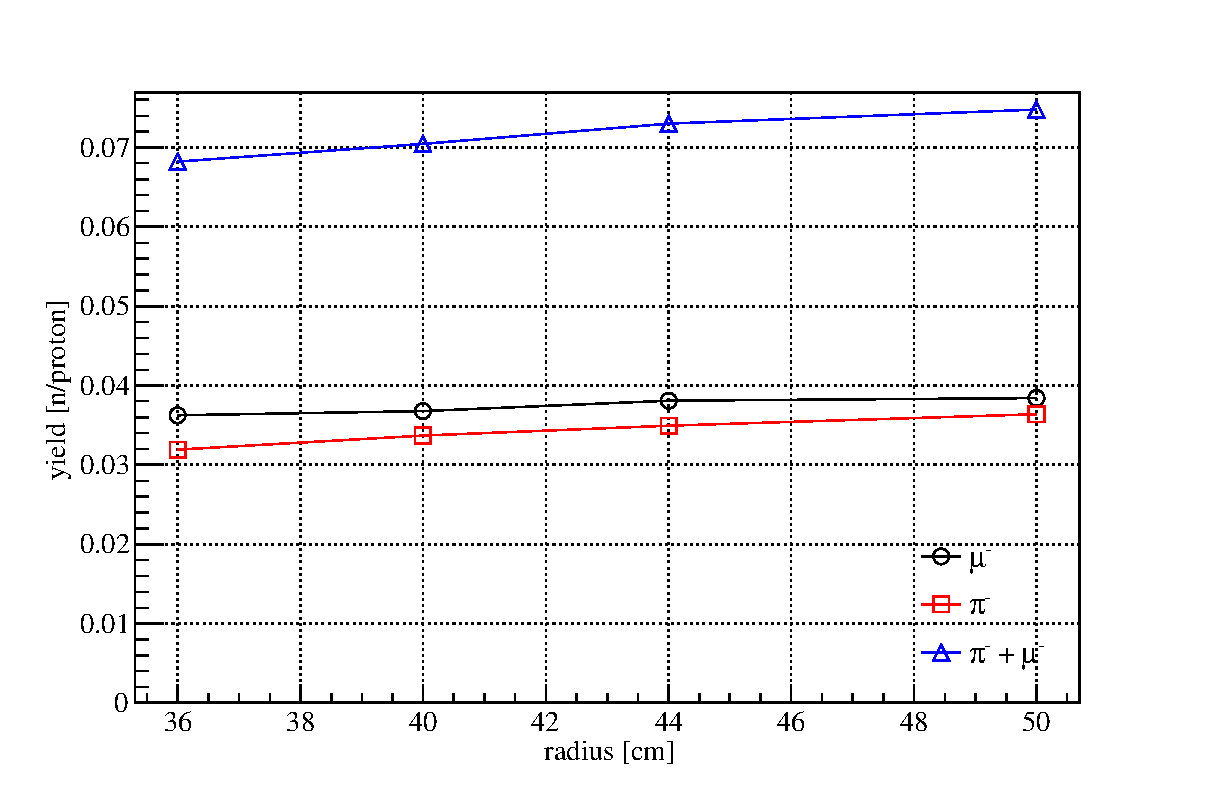
\includegraphics[scale=0.43]{chapter3/fig/muon}
 \caption{A relation of muon and pion yield with shielding backward radius. Current shielding backward radius is 36 cm. Black line: $\mu^-$, red line: $\pi^-$, blue line: $\mu^- + \pi^-$.}
 \label{radius}
\end{figure}


  \chapter{Irradiation test for superconducting magnet material}
~~~~~Since the superconducting solenoid of COMET experiment is exposed under the high radiation environment, the superconducting solenoid has a risk of quench due to the radiation damage in the some part of solenoid.
Thus, the study of radiation damage on the material used in COMET superconducting magnet system is quite significant.
In this chapter, the irradiation test on GFRPs, Quench protection diode and pure aluminium will be introduced.

 \section{Glass Fiber Reinforced Plastic}
~~~~~Glass Fiber Reinforced Plastics (GFRP) are widely used in many engineering applications because of their superior properties such as higher specific strength, specific modulus, anti-corrosion and thermal insulation~\cite{gfrp}.
In the case of COMET experiment, GFRPs are employed as the insulation spacer for superconducting magnets which suffer high magnetic field and radiation.
Due to the worse radiation resistance for the Glass-Epoxy (G10), 3 kinds of GFRPs what impregnate the Bismaleimide-Triazine (BT), Bismaleimide (BMI) and Cyanate Ester (CE) in the S-2 glass fiber have been developed to enhance the radiation resistance and mechanical properties.
Here Boron is excluded from the S-2 glass in order to reduce the influence from neutron.

 \subsection{Experiment}
~~~~~Each sample of GFRPs (G10, CE, BT and BMI) is prepared as Japanese Industrial Standards (JIS), which is with 100 mm long, 10 mm wide and 0.5 mm thick.
The irradiation test of GFRPs is taken in the Takasaki Advanced Radiation Research Institute by using 1 MeV uniform electron beam and Research Reactor Institute, Kyoto University (KUR) by using 34 MeV accelerator electron beam.
After irradiation, the tensile strength of irradiated samples is measured as well.
Figure~\ref{3samplegfrp} shows how GFRP samples break after irradiation.

For the 1 MeV electron irradiation test, radiation dose is measured by cellulose triacetate (CTA) tape~\cite{cta} and it can be estimated from the equation as follows.
\begin{equation}
 dose = \frac{D_e - D_0}{K} \cdot \frac{0.125}{t} \cdot f
\end{equation}
where the unit of dose is kGy.
$D_e$ and $D_0$ is the light absorption before and after irradiation.
$K$ is the constant for irradiation which is defined to 0.0063 for electron and 0.0081 for photon.
$t$ and $f$ are the thickness of CTA tape and correction term, respectively.
Average radiation dose is about 0.8 kGy/sec$\cdot$mA in terms of this equation.
Each sample of G10, CE, BT and BMI is irradiation with 50, 100 and 200 MGy totally.
As the results shown in figure~\ref{3resultgfrp} (left), BT and BMI are definitely stronger than G10 and CE without irradiation.
The tensile strength of G10 and CE drops to about 150 MPa after 200 MGy irradiation.
Similarly, BMI also has a tendency to degrade.
While the BT, the tensile strength has no big change after 200 MGy irradiation.
 \begin{figure}[H]
  \begin{subfigure}{0.22\textwidth}
   \centering
   \includegraphics[scale=0.28]{chapter4/fig/gfrp.eps}
  \end{subfigure}
  \hspace{0.2\textwidth}
  \begin{subfigure}{0.22\textwidth}
   \centering
   \includegraphics[scale=0.33]{chapter4/fig/broke.eps}
  \end{subfigure}
  \caption{GFRP samples before the irradiation are shown on the left. The samples are tensioned until break after irradiation (right).}
  \label{3samplegfrp}
 \end{figure}
\begin{figure}[H]
  \begin{subfigure}{0.3\textwidth}
   \centering
   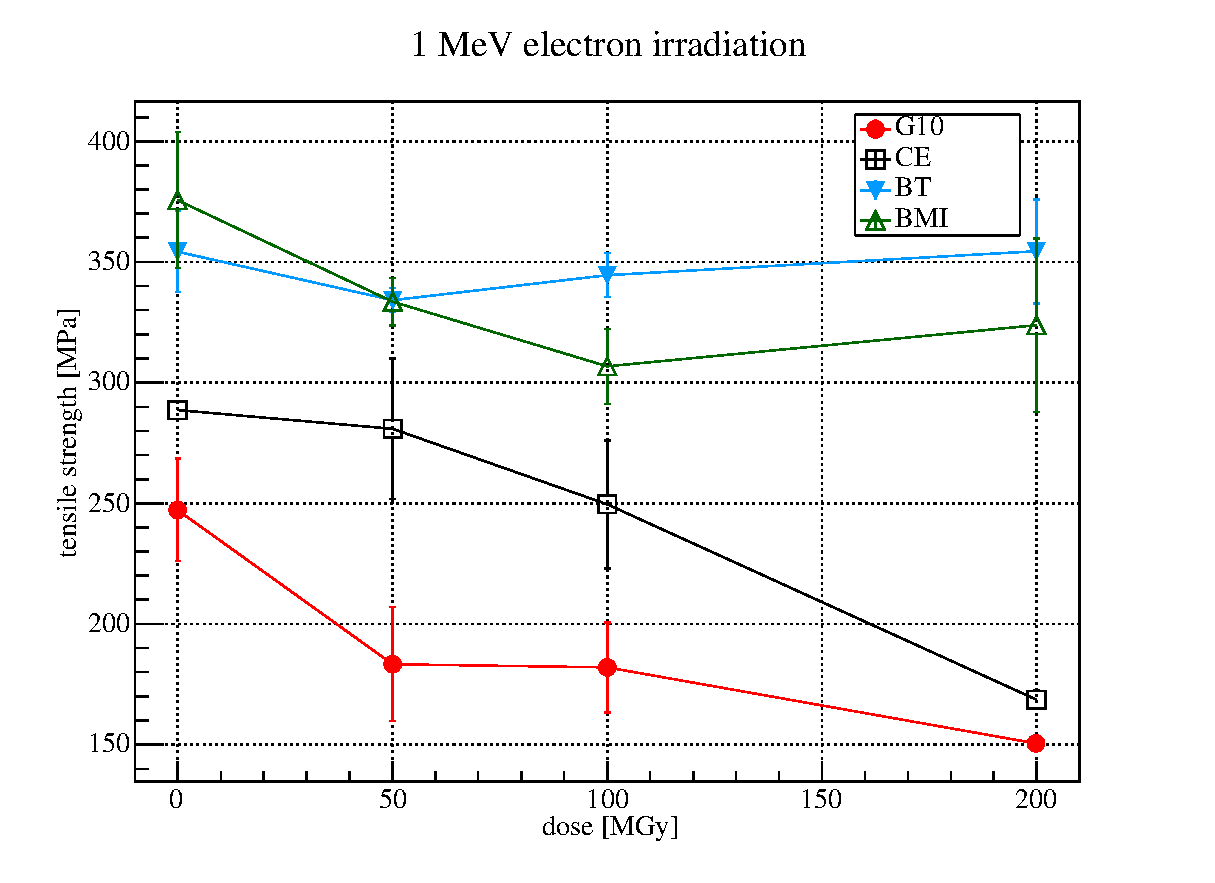
\includegraphics[scale=0.43]{chapter4/fig/tensile_takasaki.eps}
  \end{subfigure}
  \hspace{0.2\textwidth}
  \begin{subfigure}{0.3\textwidth}
   \centering
   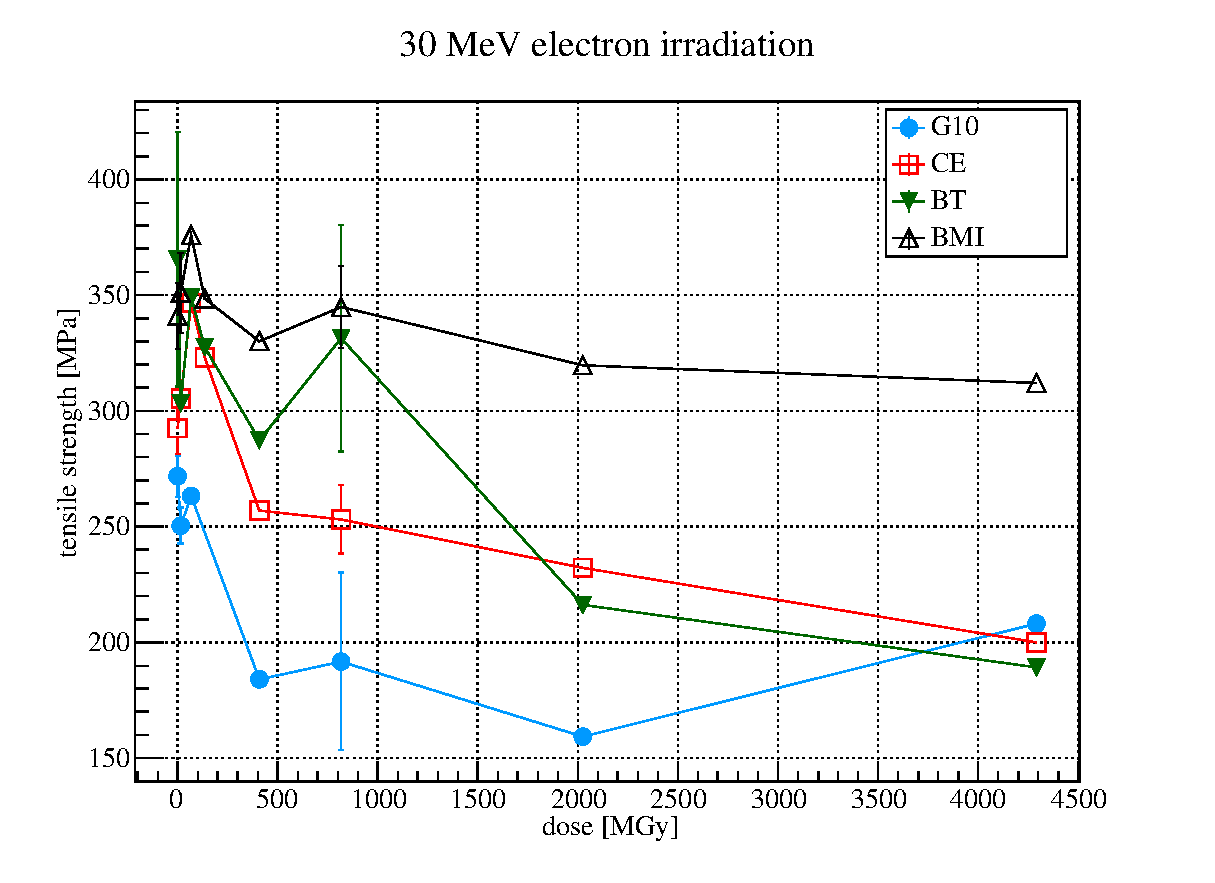
\includegraphics[scale=0.43]{chapter4/fig/tensile_kyoto.eps}
  \end{subfigure}
  \caption{The tensile strength of irradiated samples (G10, CE, BMI and BT) when it breaks. Left and Right figure represent 1 MeV electron irradiation test in JAEA, Takasaki and 30 MeV electron irradiation test in LINAC, KURRI.}
  \label{3resultgfrp}
 \end{figure}
To investigate the reaction of high energy electron on GFRPs, irradiation with 34 MeV electron has been tested by using accelerator.
Because of the electron with high energy, not only the electron but also the photon from Bremsstrahlung and neutron from the photonuclear reaction interact on GFRPs.
LINAC accelerator at KUR provides a gaussian beam with the width of 30 mm.
GFRP sample is cooled by water during the irradiation (30$^{\circ}$C).
Unlike to the 1 MeV irradiation, CTA tape is unable to be used to measure the radiation dose because its energy is out of the range of the measurement ability of CTA tape.
Thus, in this case, radiation dose is estimated by PHITS code, which is 1.25 kGy/sec$\cdot$mA.
Each sample is irradiated with 9, 30, 45, 90, 270, 540, 1340 and 2840 MGy totally.
In figure~\ref{3resultgfrp}, all samples start to degrade from 90 MGy and they drop to around 200 MPa besides BMI.
The flexural strength test and outgasing test for GFRPs are described in reference~\cite{takasaki}.
Considering the mechanical property, outgasing and radiation resistance, BT will be employed as insulation spacer in COMET superconducting magnets.

% \section{Stabilizer and conductor}
%The early radiation induced damage on superconductors with reactor neutron is studied at cryogenic temperature by Weber~\cite{weber}.
%The results show that the critical current density of NbTi drops from 10$^{22}$ n/m$^2$ high energy neutron irradiation at 5 Tesla.
 \section{Quench protection diode}
~~~~~Quench protection diode is a switch of the dump resistor.
When magnets quench, the power supply will be cut off, then this diode will be turned on and current will flow toward the dump resistor.
The operating voltage will increase after irradiation~\cite{hagedorn}, which causes the over heat of quench protection diode.
Moreover different manufacturer fabricates diode with different electrical property.
Here, a dedicated quench protection diode for COMET superconducting magnet has been irradiated by high energy neutron.
Its electrical characteristics under low temperature and radiation is investigated.

  \subsection{Experiment}
~~~~~The irradiation test for quench protection diode is taken with COMET detector group together at the Tendem accelerator, Kyushu university.
The fast neutron is produced from carbon target with incident 9 MeV deutron, which creates neutron by deutron-deutron reaction.
5 kinds of samples are set up in front of the production target with the distance of 3 cm as the sequence of MPPC, APD, Artix-7, ROESTI and diode, which is shown in figure~\ref{3setup}.
 \begin{figure}[H]
  \centering
  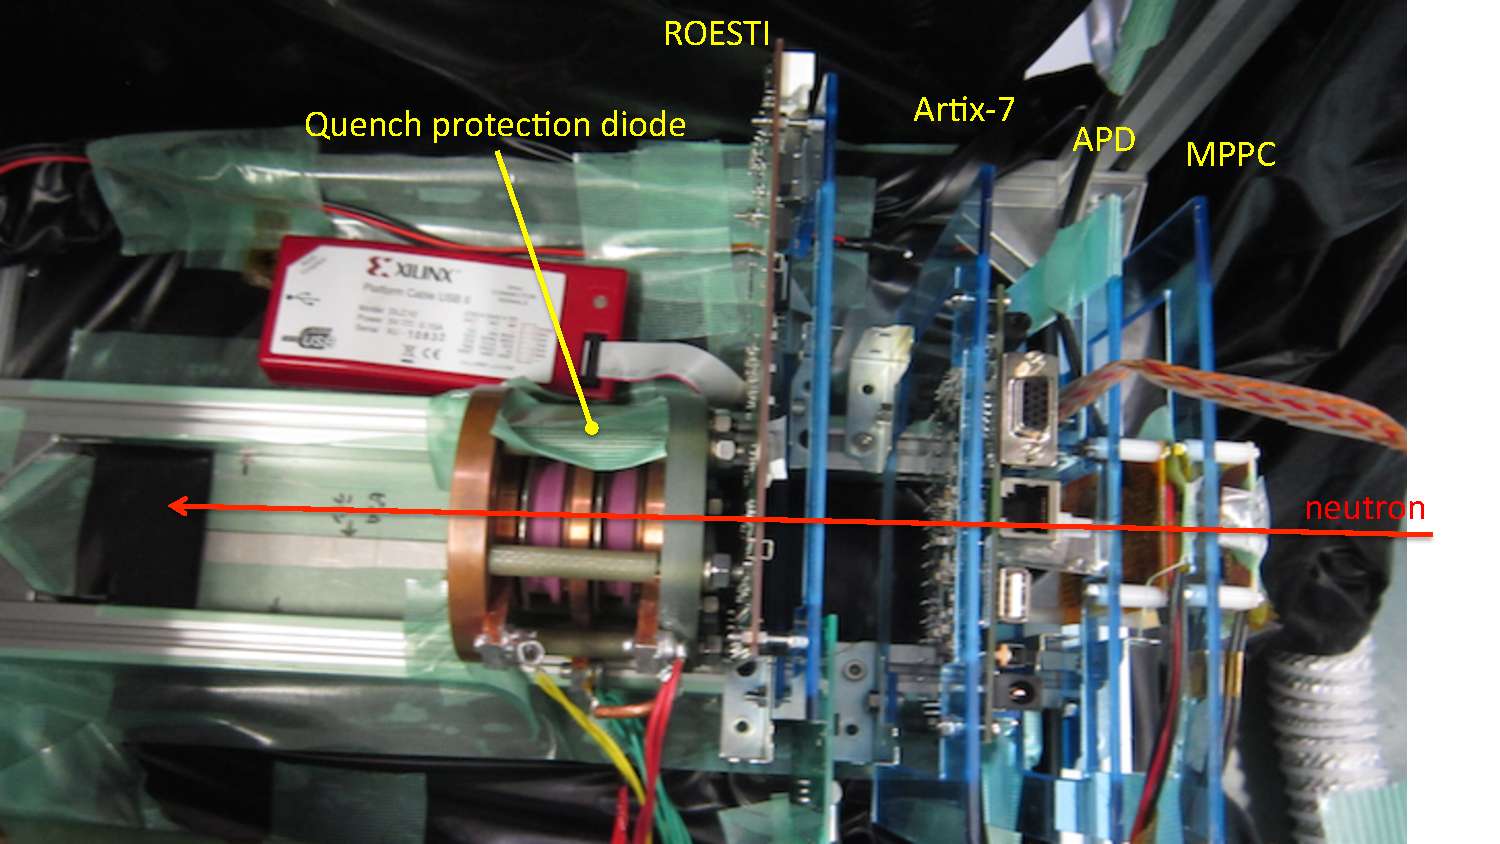
\includegraphics[scale=0.45]{chapter4/fig/diodepic.pdf}
  \caption{Sample setup for neutron irradiation test. Diode is set up in front of MPPC, APD, Artix-7 and ROESTI where is 30 cm far from the neutron production target.}
  \label{3setup}
 \end{figure}
Because diode is with the radius of 3 cm and length of 10 cm, which is possible to stop the neutron, it is located at last of samples where 30 cm far from the production target.
Its turn-on voltage is measured during the irradiation with 5 A power supply, and neutron flux is measured by activation analysis with aluminium, nickel and gold wire (0.07\% Fe).
Temperature of diode during the irradiation is recorded by thermometer.
  
  \subsection{Neutron measurement}
~~~~~Activation analysis is a common and easy way of neutron measurement, but with the bad energy resolution.
aluminium, nickel and gold wire (0.07\% Fe) are employed and stuck on the surface of each sample.
The photon from neutron reaction on each activation sample which is list in table~\ref{act} is measured by HPGe detector.
\begin{table}[H]
 \centering
 \begin{tabular}{ccccc} \hline \hline
  Element & Reaction & Threshold energy & Half life & Emitted radiation energy [MeV] \\ \hline
  aluminium & $^{27}$Al(n, p)$^{27}$Mg & 1.9 MeV & 9.46 min & $\beta^-$ (1.75), $\gamma$ (0.84, 1.013) \\
  aluminium & $^{27}$Al(n, $\alpha$)$^{24}$Na & 3.27 MeV & 15 h & $\beta^-$ (1.389), $\gamma$ (1.369, 2.754) \\
  Gold & $^{197}$Au(n, $\gamma$)$^{198}$Au & (-) & 2.7 d & $\beta^-$ (0.962), $\gamma$ (0.412) \\
  Gold & $^{197}$Au(n, 2n)$^{196}$Au & 7.36 MeV & 6.18 d & $\beta^-$, $\gamma$ (0.356) \\
  Nickel & $^{58}$Ni(n, 2n)$^{57}$Ni & 12.09 MeV & 36 h & $\beta^+$, $\gamma$ (0.511, 1.37) \\ \hline \hline
 \end{tabular}
 \caption{Neutron activation reactions.}
 \label{act}
\end{table}
  \begin{figure}[H]
   \begin{subfigure}{0.3\textwidth}
    \centering
	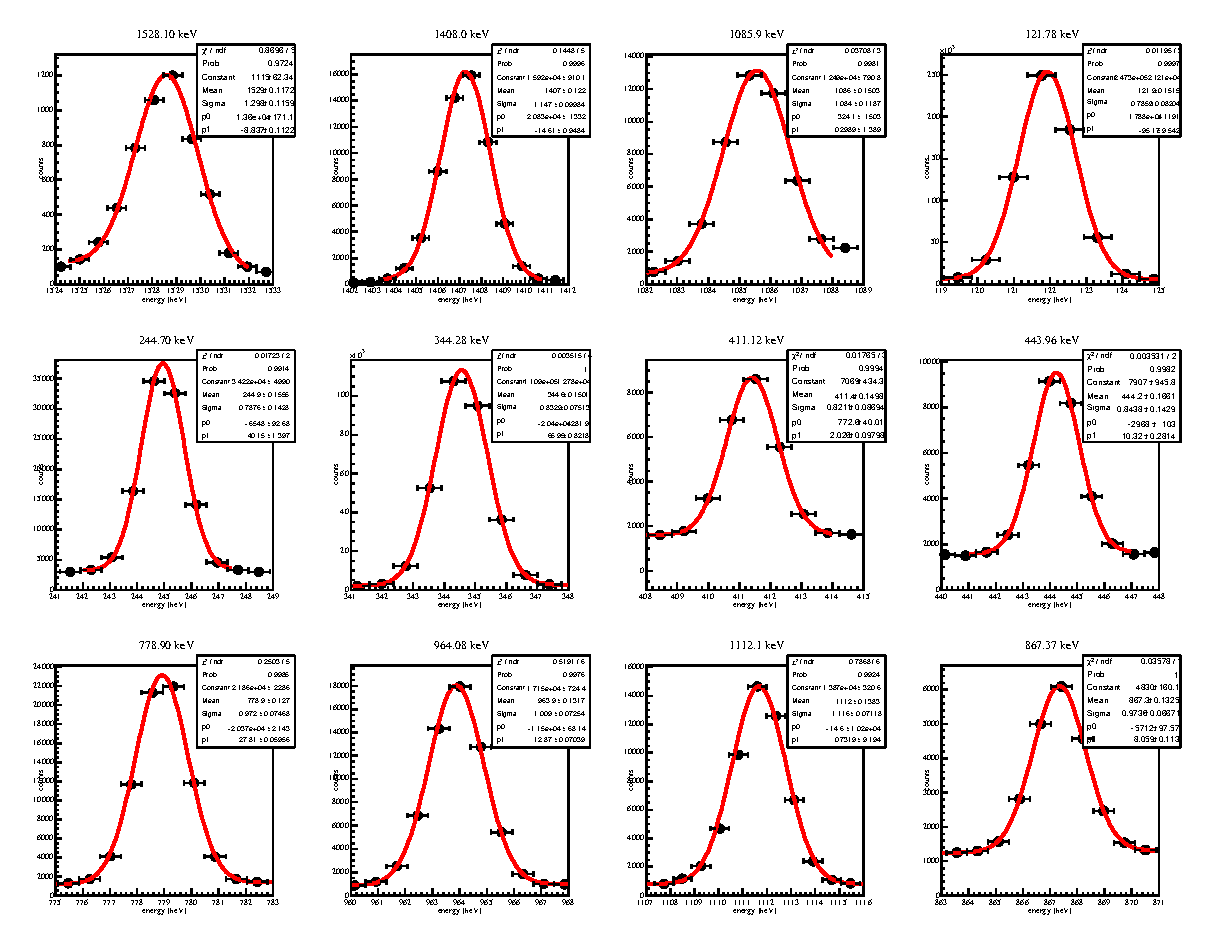
\includegraphics[scale=0.46]{chapter4/fig/Eufit.eps}
   \end{subfigure}
   \hspace{0.25\textwidth}
   \begin{subfigure}{0.3\textwidth}
    \centering
	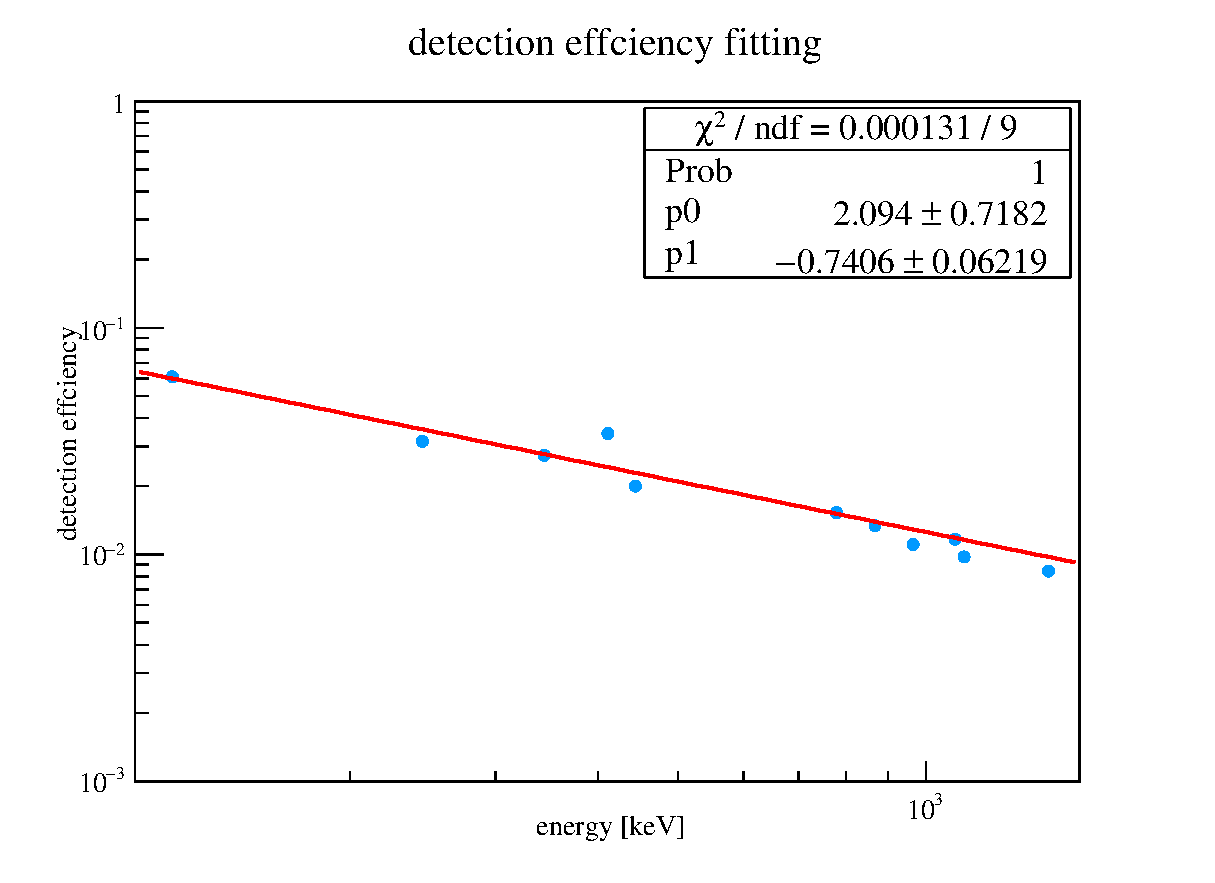
\includegraphics[scale=0.35]{chapter4/fig/detectioneff.eps}
   \end{subfigure}
   \caption{The detection efficiency is calibrated by using $^{152}$Eu radiation source. Several peak of $^{152}$Eu is fitted as convolution on left, and the detection efficiency of HPGe is fitted on right.}
   \label{3source}
  \end{figure}
$^{152}$Eu with 2.79$\times$10$^7$ Bq is employed as the calibration source to estimate the detection efficiency of HPGe detector.
As shown in figure~\ref{3source}, each peak of radiation source $^{152}$Eu is fitted as gaussian and linear function.
The detection efficiency is fitted as
\begin{equation}
 \epsilon = a \cdot E^b
\end{equation}
where the counts for the calculation of detection efficiency $\epsilon$ is within 1.78$\sigma$.
\begin{table}[H]
 \centering
 \begin{tabular}{cc} \hline \hline
  a & b \\ \hline
  2.094$\pm$0.7182 & -0.7406$\pm$0.06219 \\ \hline \hline
 \end{tabular}
 \caption{Fitting parameters for detection efficiency.}
\end{table}

%  \begin{figure}[H]
%   \centering
%   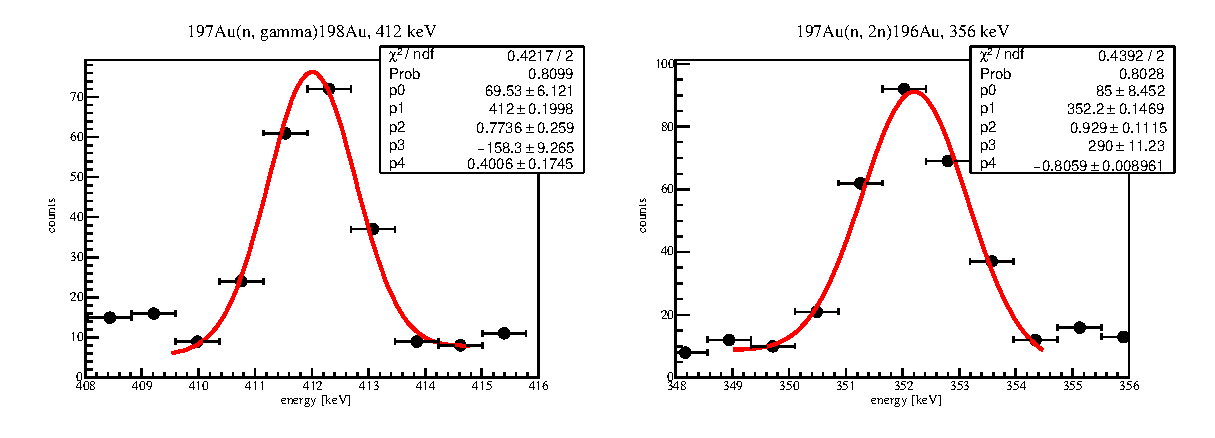
\includegraphics[scale=0.45]{chapter4/fig/aupeak}
%   \caption{ The peak of $^{197}$Au decay on the diode downstream.}
%   \label{3nipeak}
%  \end{figure}

Neutron flux measured by each activation sample is given by~\cite{nicholas}
\begin{equation}
 \phi = \frac{C \cdot A \cdot \lambda}{\sigma \cdot N_A \cdot \gamma \cdot m \cdot I \cdot \epsilon \cdot (1 - e^{-\lambda t_0}) \cdot (e^{-\lambda t_1} - e^{-\lambda t_2})}
\end{equation}
where $C$ is the number of counts under the peak of each activation sample.
$\sigma$ and $\gamma$ are the cross section of a reaction which is picked up from JENDL data library and probability that a photon is emitted per decay of the isotope respectively.
$N_A$ is the Avogadro constant, and $I$ is a weight fraction of isotope with atomic mass $A$.
$m$ is the mass of activation sample.
$\epsilon$ and $t_2-t_1$ are the detection efficiency and counting time.
  \begin{figure}[H]
   \begin{subfigure}{0.3\textwidth}
   \centering
   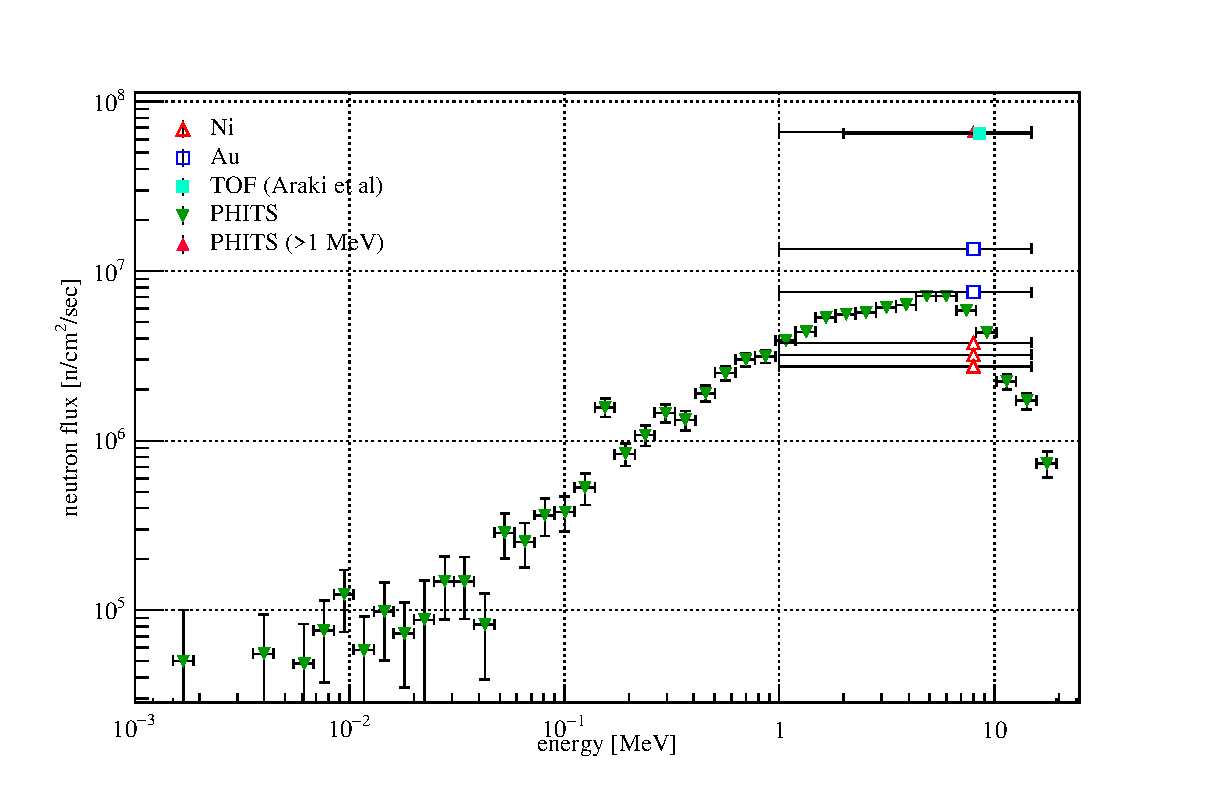
\includegraphics[scale=0.45]{chapter4/fig/flux}
   \end{subfigure}
   \hspace{0.2\textwidth}
   \begin{subfigure}{0.3\textwidth}
   \centering
   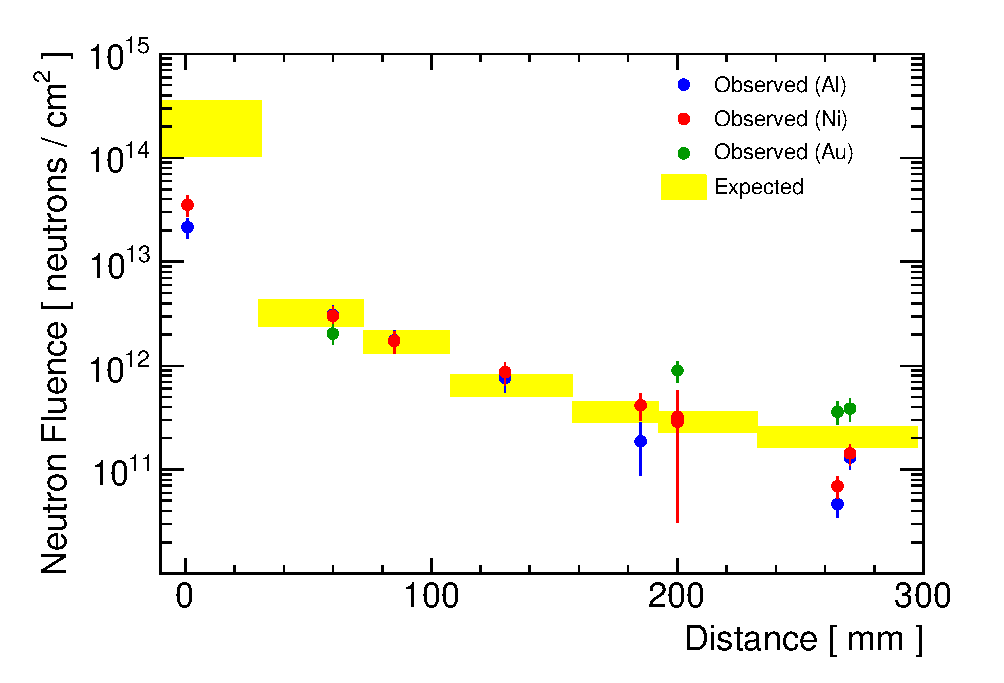
\includegraphics[scale=0.48]{chapter4/fig/fluxtot.pdf}
   \end{subfigure}
   \caption{Neutron flux is measured by Au wire, Al and Ni foils. The comparison of experimental data with simulation (left). The neutron flux on the place where samples are set up is shown on rihgt.}
   \label{3flux}
  \end{figure}

As shown in figure~\ref{3flux}, neutron flux on diode measured by gold wire is higher nickel's, which is 1.35$\times$10$^7$ n/cm$^2$/sec.
From the prediction of PHITS code and previous measurement with liquid scintillator, the neutron flux is 6$\times$10$^7$ n/cm$^2$/sec which is about 5 times higher than the measurement of gold wire.
It is possible that a part of neutron is stopped at flange or the other irradiation sample and causes the different between measurement and prediction.
Thus, in this case, we trust the measurement and the total neutron fluence irradiated until the end of experiment is estimated for 10$^{12}$ n/cm$^2$/sec.

  \subsection{Electrical property of diode}
~~~~~To investigate the electrical properties of diode, the turn-on voltage is measured during the irradiation, then the voltage on the operating current is predicted by fitting the V-I curve of diode.
The relation of turn-on voltage (forward voltage at 100 mA) and neutron fluence is shown in figure~\ref{3switch}.
It reduces with neutron fluence and slope of V-I curve becomes bigger after irradiation.
Temperature from the beginning of the experiment until the end of the experiment is controlled around 25.6$^{\circ}$C.

Figure~\ref{3fitdiode} shows the fitting for each V-I curve as the function~\ref{dioeq}, and fitting parameters are listed in table~\ref{fit3}.
\begin{equation}
 I = I_0 (e^{-V/V_T} - 1)
\label{dioeq}
\end{equation}
where $I$ and $V$ are the diode current and voltage across the diode.
$V_T$ is thermal voltage and $I_0$ is the saturation current, which are assumed the fitting parameters here.
  \begin{figure}[H]
   \begin{subfigure}{0.3\textwidth}
    \centering
	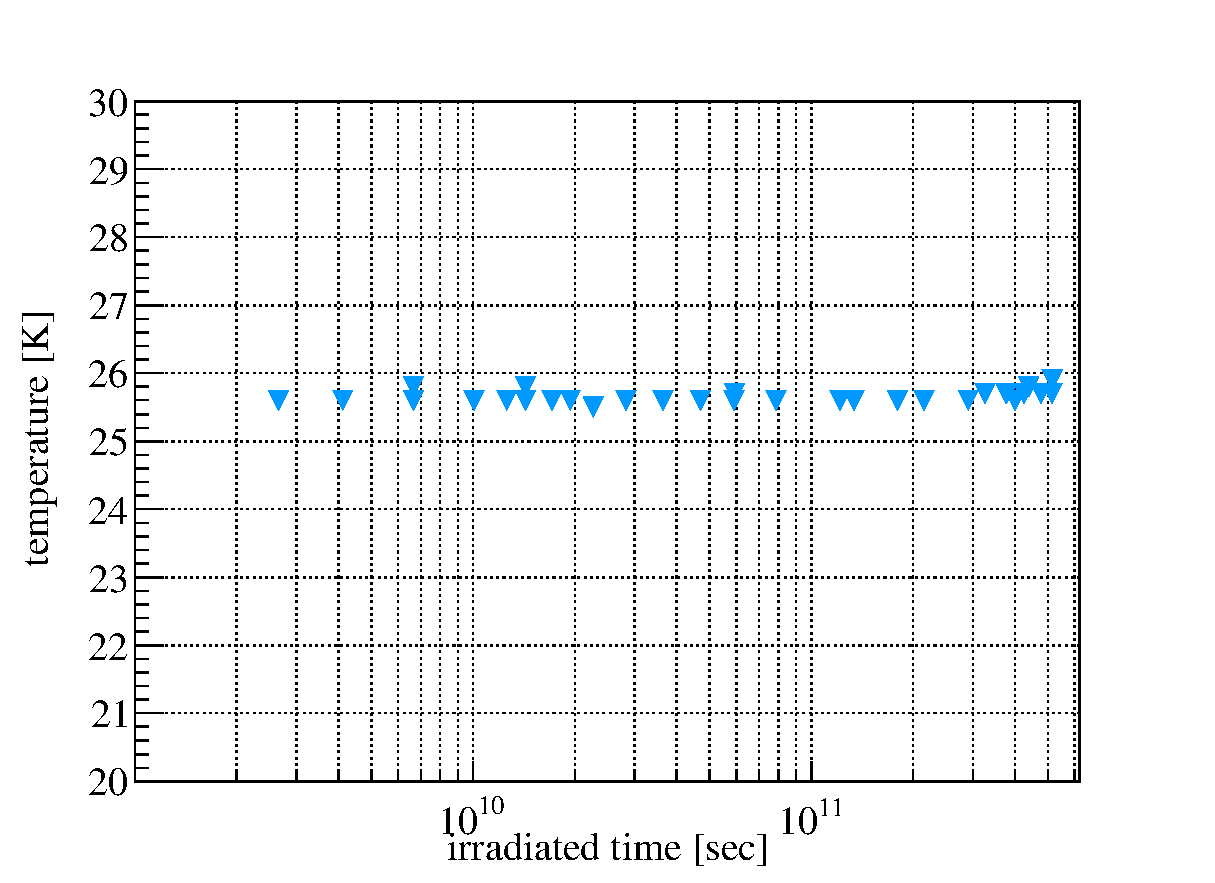
\includegraphics[scale=0.43]{chapter4/fig/temperature.eps}
   \end{subfigure}
   \hspace{0.2\textwidth}
   \begin{subfigure}{0.3\textwidth}
    \centering
	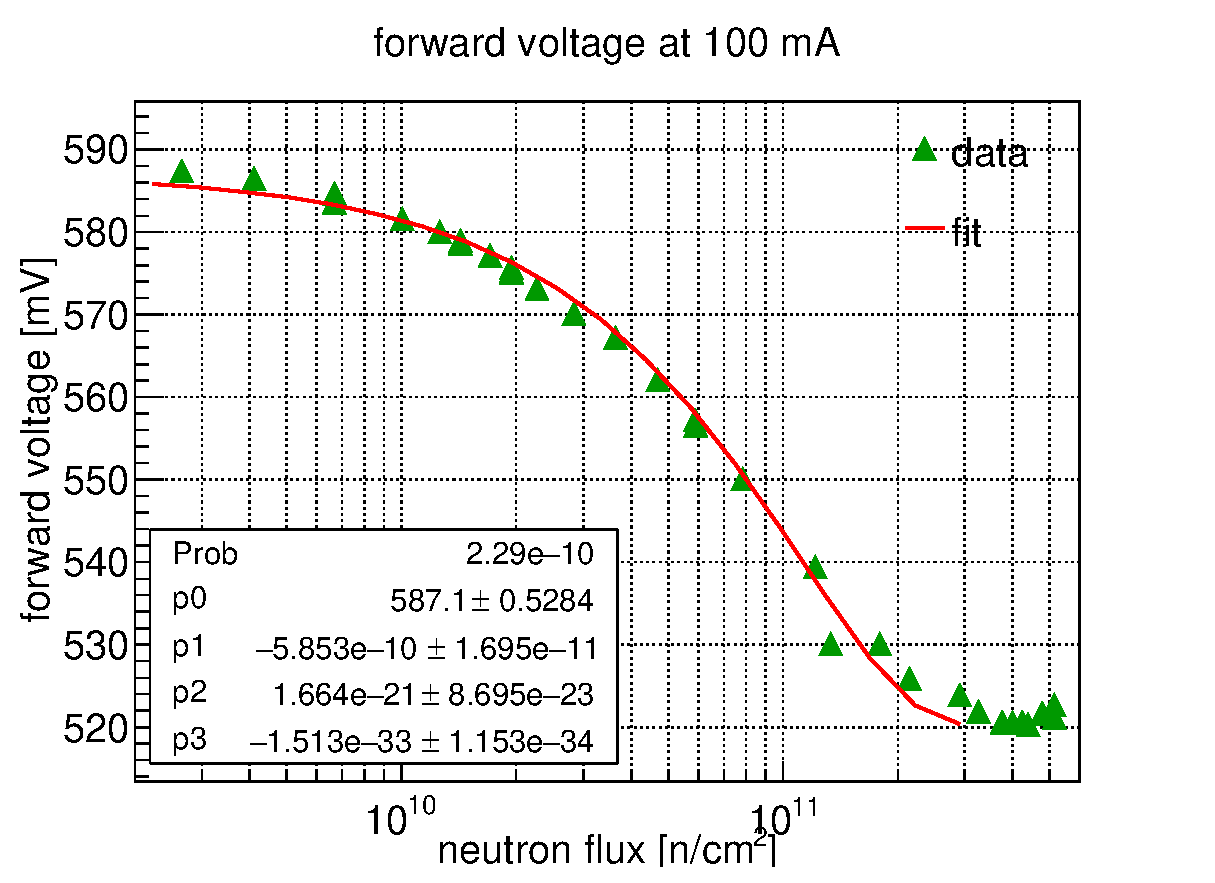
\includegraphics[scale=0.43]{chapter4/fig/switchon.eps}
   \end{subfigure}
   \caption{The temperature during the irradiation (left). The turn-on voltage decreases with the neutron fluence (right).}
   \label{3switch}
  \end{figure}
  \begin{figure}[H]
   %\begin{subfigure}{0.3\textwidth}
    \centering
    \includegraphics[scale=0.45]{chapter4/fig/diodefit.eps}
   %\end{subfigure}
   %\hspace{0.2\textwidth}
   %\begin{subfigure}{0.3\textwidth}
   % \centering
	%\includegraphics[scale=0.43]{chapter4/fig/fit210}
   %\end{subfigure}
   \caption{Measured turn-on voltage for quench protection diode. It is fitted as diode V-I function. Black and green point represent the original V-I curve and V-I curve after 10$^{12}$ n/m$^2$ irradiation.}
   \label{3fitdiode}
  \end{figure}
 
\begin{table}[H]
 \centering
 \begin{tabular}{cccccc} \hline \hline
  irradiated time [sec] & I$_0$ & V$_T$ & irradiated time [sec] & I$_0$ & V$_T$ \\ \hline
  0 & 2.04883$\times$10$^{-7}$ & 23.0918 & 500 & 1.97681$\times$10$^{-7}$ & 23.034 \\
  1064 & 2.73547$\times$10$^{-7}$ & 22.6213 & 1505 & 3.75863$\times$10$^{-7}$ & 22.2084 \\
  4274 & 1.35549$\times$10$^{-6}$ & 20.5447 & 9884 & 5.35415$\times$10$^{-6}$ & 18.7640 \\
  14008 & 9.77339$\times$10$^{-6}$ & 17.9582 & 68468 & 4.15128$\times$10$^{-5}$ & 15.7070 \\ \hline \hline
 \end{tabular}
 \caption{Fitting parameters for V-I curve.}
 \label{fit3}
\end{table}

 \subsection{Electrical property at cryogenic temperature}
~~~~~Since Quench protection diode is connected to the magnets with superconducting wire, the diode must be cooled to the temperature same as superconducting wire, 4.2 K.
Therefore, the electrical property at cryogenic temperature needs to be investigated as well.

For the measurement at cryogenic temperature, Quench protection diode is cooled directly by liquid nitrogen at 77 K which shown in figure~\ref{3cryotemp}.
Unlike to the result of irradiation, not only the turn-on voltage but also the V-I curve increases in 77 K.
In figure~\ref{3cryo}, the V-I curve at 300 K and 7 K can be fitted by
\begin{table}[H]
 \centering
 \begin{tabular}{cccccc} \hline \hline
  Temperature [K] & I$_0$ & V$_T$ &Temperature [K] & I$_0$ & V$_T$ \\ \hline
  300 & 8.088$\times$10$^{-7}$ & 21.05 & 77 & 1.969$\times$10$^{-12}$ & 25.95 \\ \hline \hline
 \end{tabular}
 \caption{Fitting parameters for forward voltage of diode at 300 K and 77 K.}
 \label{fit4}
\end{table}
Using this fitting parameters, the forward voltage at 300 K and 77 K can be predicted to 0.92 V and 1.25 V respectively.
Compared with the case of room temperature, 0.33 V is increased during the cooling.
 \begin{figure}[H]
  \centering
  \includegraphics[scale=0.35]{chapter4/fig/cryotemp.pdf}
  \caption{Measurement of the forward voltage of diode at cryogenic temperature.}
  \label{3cryotemp}
 \end{figure}

\subsection{Forward voltage at 210 A}
~~~~~~Since the operating current for transport solenoid is 210 A, a relation between fitted forward voltage at 210 A and neutron fluence is shown in figure~\ref{3diode}.
The forward voltage increases following the neutron fluence which is assumed as the exponential function.
\begin{equation}
 V = exp(-0.09373 + 8.832 \times 10^{-14} \cdot \phi)
\end{equation}
In the case of COMET phase-II experiment, the neutron at the place of quench protection diode is about 4.02$\times$10$^5$ n/cm$^2$/sec with the energy lower than 1 MeV  according to PHITS simulation.
As for the 280-day operation, the total neutron fluence is estimated to about 9.73$\times$10$^{12}$ n/cm$^2$ for quench protection diode.
Because the displacement cross section of silicon at low energy region is lower than the case of high energy region, irradiation for 10$^{12}$ n/cm$^2$ at the range from 1 MeV reaches to the effects of 9.73$\times$10$^{12}$ n/cm$^2$ irradiation.
After 10$^{12}$ n/cm$^2$ irradiation, the forward voltage at operating current is increased 0.08 V.
  \begin{figure}[H]
   \centering
   \includegraphics[scale=0.5]{chapter4/fig/dioderesult.eps}
   \caption{Relative increase of the forward voltage versus neutron fluence at room temperature.}
   \label{3diode}
  \end{figure}

Turn-on voltage at 100 mA is proportional to the temperature linearly as
\begin{equation}
 V = 1.221 - 0.002077 \cdot T
\end{equation}
Assuming the forward voltage at 210 is also linear to the temperature, the forward voltage is predicted to 1.33 V at 4.2 K and 210 A.
Including the voltage change during the irradiation, we assume the forward voltage at 210 A and 4.2 K will increase from 0.9 V to 1.5 V.
Even if the forward voltage increases to 1.5V, the temperature rises to about 11 K during the cooling of liquid helium which is calculated by one dimensional Finite Element Method.
Without the cooling, the temperature of diode will increase up to 70 K at 10 sec.
 \begin{figure}[H]
  \begin{subfigure}{0.3\textwidth}
   \centering
   \includegraphics[scale=0.43]{chapter4/fig/cryo.eps}
  \end{subfigure}
  \hspace{0.2\textwidth}
  \begin{subfigure}{0.3\textwidth}
   \centering
   \includegraphics[scale=0.43]{chapter4/fig/temp.eps}
  \end{subfigure}
  \caption{Forward V-I curve measured at room temperature and nitrogen temperature without irradiation (left). The measurement of turn-on voltage at 100 mA from room temperature to 77 K (right).}
  \label{3cryo}
 \end{figure}

 \section{Insulation tape}
%~~~~~The conduct is commonly covered with several polyimide tapes as ground insulation between two conducts.
%As for the COMET superconducting magnets, 4 kinds of insulation tape, BTGU, BTGK-A, BTGK-B, BTGK-C, are developed to enhance the mechanical property and radiation resistance.
~~~~~~The conductor of pion capture solenoid is wound by two layers of insulation tape so called pre-preg tape as ground insulation.
This insulation tape shown in figure~\ref{3stur} is made of polyimide film covered by boron free glass with BT and epoxy resin to enhance the mechanical property under the high radiation environment.
 \begin{figure}[H]
  \begin{subfigure}{0.3\textwidth}
  \centering
  \includegraphics[scale=0.36]{chapter4/fig/prepreg.pdf}
  %\caption{ The structure of pre-preg tape.}
  \label{3stur}
  \end{subfigure}
  \hspace{0.2\textwidth}
  \begin{subfigure}{0.3\textwidth}
  \centering
  \includegraphics[scale=0.31]{chapter4/fig/BUGT.pdf}
  %\caption{ Tensile test for pre-preg tape.}
  \label{3break}
  \end{subfigure}
  \caption{Insulation tape is made of glass cross and polyimide film impregnated by BT and epoxy resin (left). The two pieces of insulation tapes are sandwiched with aluminium strip to take tensile test (right).}
 \end{figure}
Four samples, BTGU, BTGK-A, BTGK-B and BTGK-C, made of same material but different rate of BT and epoxy resin are prepared for tensile test.
Here, mixing the BT and epoxy resin with different rate can adjust the viscosity of insulation tape.
Two samples are struck and sandwiched with aluminium strip (Al-GU-UG-Al) as JIS standards for tensile test are cured by 170$^{\circ}$C and 8 hours.
Figure~\ref{3break} shows how the pre-preg tape breaks after tensile test.
The result of tensile test for the sample without irradiation is given in figure~\ref{3gubt}, which shows the BTGK-C is the strongest one in these sample.
However, the glass layer and resin layer is not struck before the thermal process, which is hard to employ it as the insulation tape in superconducting coil.
Considering the mechanical properties may reduce after irradiation, the irradiation of BTGU samples is taken in Takasaki Advanced Radiation Research Institute with cobalt radiation source.
As the result shown in figure~\ref{3gubt} (right), the tensile strength of BTGU sample does not reduce after irradiation, however, surprisingly, the tensile strength increases about 10\% after 10 MGy irradiation.
 \begin{figure}[H]
  \begin{subfigure}{0.3\textwidth}
   \centering
   \includegraphics[scale=0.43]{chapter4/fig/gubt.eps}
  \end{subfigure}
  \hspace{0.2\textwidth}
  \begin{subfigure}{0.3\textwidth}
   \centering
   \includegraphics[scale=0.43]{chapter4/fig/BTGU2.eps}
  \end{subfigure}
  \caption{3 samples of each BTGU, BTGK-A, BTGK-B and BTGK-C are tensioned without irradiation (left). BTGU shows no degradation after irradiated with 10 MGy at limit by cobalt $\gamma$ ray source.}
  \label{3gubt}
 \end{figure}

 \section{Radiation test for conductor}
~~~~~~The degradation of electrical resistivity occurs when the stabilizer irradiated by radiation due to the production of Frenkel pairs.
In the cryogenic temperature, since the displaced atoms are difficult to return to the defect, a depletion region is possible to be generated under the long time irradiation.
Radiation damage effects of conductor are necessary to investigate because it may cause the overheat of superconducting coils due to the RRR decreasing and quench.
\begin{figure}[H]
 \begin{subfigure}{0.3\textwidth}
  \centering
  \includegraphics[scale=0.43]{chapter4/fig/yield.eps}
 \end{subfigure}
 \hspace{0.2\textwidth}
 \begin{subfigure}{0.3\textwidth}
  \centering
  \includegraphics[scale=0.43]{chapter5/fig/AlDPA.eps}
 \end{subfigure}
 \caption{all kinds of particles which hit the CS1 coil (left). The displacement cross section of aluminium for neutron (right).}
 \label{3yield}
\end{figure}
To ensure what kinds of particle hit the superconducting coils, the simulation is taken by PHITS and its yield is shown in figure~\ref{3yield}.
Compared with the other particles, the neutron is most biggest issue for superconducting coils.
Furthermore, the energy of neutron in the range from 0.1 MeV dominates the radiation damage, which is about 100 b.
Thus, irradiation test of pure aluminium and copper for conductor is studied in Kyoto University Research Reactor Institute (KURRI) with reactor neutron.
The pure aluminium and copper samples are set up in the one of beamline from reactor where can irradiate with cryogenic temperature.
Neutron fluence is 1.4$\times$10$^{11}$ n/m$^2$/sec for fast neutron in terms of the KUR study~\cite{kur}.
Figure~\ref{4dpa} shows the energy spectrum at center of reactor, which is higher than the place where we take irradiation test with factor 30.34.
  \begin{figure}[H]
    \centering
	\includegraphics[scale=0.43]{chapter5/fig/neutron.eps}
   \caption{Neutron spectrum at core of KUR reactor.}
   \label{4dpa}
  \end{figure}
As the result, we obverse that the resistivity increases about 0.03 n$\Omega\cdot$m for aluminium and 0.01 n$\Omega\cdot$m for copper after after 10$^{20}$ n/m$^2$ neutron irradiation.
Thus, due to the neutron induced resistivity, the resistivity of stabilizer at cryogenic temperature should be modified as
\begin{equation}
 \rho (T) = \rho_0(T) + \bigtriangleup \rho_{n} (\Phi) + \bigtriangleup \rho_{mag} (B)
\end{equation}
where $\rho_0(T)$ is the resistivity at cryogenic temperature without magnetic field and irradiation.
$\bigtriangleup \rho(\Phi)$ and $\bigtriangleup \rho(B)$ are the neutron induced resistivity which depends on the neutron fluence and magnetoresistivity, respectively.
Thus, the RRR during the irradiation is given by
\begin{equation}
 RRR = \frac{\rho_{RT}}{\rho_0 + f \cdot \phi \cdot t}
\end{equation}
where the factor $f$ is shown in table~\ref{factorirr}.
\begin{table}[H]
 \centering
 \begin{tabular}{cc} \hline \hline
  Element & Factor [n$\Omega\cdot$m$^3$] \\ \hline
  aluminium & 3$\times$10$^{-22}$ \\
  Copper & 1$\times$10$^{-22}$ \\ \hline \hline
 \end{tabular}
 \caption{Factor for the neutron induced resistivity.}
 \label{factorirr}
\end{table}
Since the aluminium with RRR of 2000 and 400 will be employed as strip and stabilizer respectively, the relation between RRR and neutron fluence is shown in figure~\ref{4rrr}.
The RRR of aluminium strip and stabilizer for 280-day operation will become 40 or lower for capture solenoid according to the maximum neutron fluence of 2$\times$10$^{21}$ n/m$^2$ which is predicted by PHITS code (JAM\_INCL4.6\_JENDL4 model).
Details of RRR degradation for main superconducting magnets of pion capture solenoid is listed in table~\ref{RRRdeg} and figure~\ref{4rrr} (right).
\begin{table}[H]
 \centering
 \begin{tabular}{ccccc} \hline \hline
  Name & neutron flux [n/cm$^2$/sec] & DPA [DPA/280 days] & RRR (Al strip) & RRR (stabilizer) \\ \hline
  CS0 & 1.03$\times$10$^{10}$ & 3.44$\times$10$^{-5}$ & 39 & 36 \\
  CS1 & 5.12$\times$10$^{9}$ & 2.97$\times$10$^{-5}$ & 77 & 67 \\
  MS1 & 4.11$\times$10$^{9}$ & 1.82$\times$10$^{-5}$ & 95 & 80 \\
  MS2 & 1.20$\times$10$^{9}$ & 8.11$\times$10$^{-6}$ & 293 & 185 \\ \hline \hline
 \end{tabular}
 \caption{Details of RRR degradation for pion capture solenoid after 280-day operation.}
 \label{RRRdeg}
\end{table}

  \begin{figure}[H]
   \begin{subfigure}{0.3\textwidth}
    \centering
	\includegraphics[scale=0.43]{chapter5/fig/degradation.eps}
   \end{subfigure}
   \hspace{0.2\textwidth}
   \begin{subfigure}{0.3\textwidth}
    \centering
	\includegraphics[scale=0.43]{chapter5/fig/rrrmagnets.eps}
   \end{subfigure}
   \caption{ Predicted the RRR-neutron curve from the neutron irradiation test in KUR.}
   \label{4rrr}
  \end{figure}

 \subsection{Discussion}
~~~~~~The radiation induced damage of material can be estimated by one parameter called Displacement Per Atom (DPA) which is given by
\begin{equation}
 DPA = \sigma_{dpa} \cdot \phi_i
\end{equation}
where $\sigma_{dpa}$ and $\phi_i$ are the displacement cross section and particle flux respectively.
The displacement cross section depends on the material, and is a predicting value.
Through the DPA, the radiation damage in different energy region is able to be compared.
Using the neutron flux and displacement cross section of aluminium in figure~\ref{3yield}, the DPA can be estimated as follows.
\begin{table}[H]
 \centering
 \begin{tabular}{cc} \hline \hline
  DPA model & DPA calculation [DPA] \\ \hline
  BCA + MD & 1.0$\times$10$^{-5}$ \\
  ABBN & 2.6$\times$10$^{-5}$ \\
  NRT (Mu2e) & 2.5$\times$10$^{-5}$ \\
  NRT (COMET) & 3.0$\times$10$^{-5}$ \\ \hline \hline
 \end{tabular}
 \caption{DPA estimation for the neutron irradiation test of pure aluminium.}
\end{table}
Here, BCA + MD, ABBN, and NRT (Mu2e) are the estimation with different DPA models from Mu2e collaboration.
Our estimation is about 3.0$\times$10$^{-5}$ DPA.
J.A. Horak et al. measure the neutron induced resistivity of metals, as a result, the induced resistivity for aluminium is 382.3 n$\Omega\cdot$cm per 5.6$\times$10$^{-4}$ Frenkel pair~\cite{horak}.
In addition, reference~\cite{yu} shows many results of Frenkel pair resistivity of aluminium in table~\ref{frank}.
\begin{table}[H]
 \centering
 \begin{tabular}{ccc} \hline \hline
  $\rho_{FP}$ [$\mu\Omega\cdot$m] & Type & Reference \\ \hline
  3.9$\pm$0.6 & Exp D & \cite{erh1} \\
  4.2$\pm$0.8 & Exp D & \cite{erh2} \\
  3.2$\pm$0.6 & Exp D & \cite{rober} \\
  3.4 & Exp T(p) & \cite{ref1} \\
  1.32 & Exp T(p) & \cite{ref2} \\
  1.35 & Exp T(p) & \cite{ref3} \\
  4.0$\pm$0.6 & Evl E & \cite{ref4} \\
  4.2$\pm$0.5 & Evl E & \cite{ref5} \\
  4.3 & Evl S & \cite{ref6} \\ \hline \hline
 \end{tabular}
 \caption{The Frenkel pair resistivity $\rho_{FP}$ of aluminium. Methods of the data derivation: Exp D is X-ray diffraction method, Exp T is the threshold energy determination for electron irradiation of single crystals at low temperature. Exp T(p) is for the electron irradiation of polycrystals, Evl S is the estimation made with the help of the systematics~\cite{yu}.}
 \label{frank}
\end{table}
It shows that J.A. Horak's data is the maximum value compared with the other references.
The relation between DPA and RRR by using these prediction from experimental data is shown in~\ref{dpaaa}.

For the COMET phase-II experiment, the DPA peak of CS1 coil is about 1.1$\times$10$^{-5}$ DPA for 280-day operation from the prediction of PHITS code with NRT model.
The aluminium strip will not degrade lower than 100 for 280-day operation from this estimation.
However, the design has to consider the worst situation for superconducting coils, the uncertainty of the prediction from neutron DPA and neutron fluence needs to be reconsidered.
\begin{figure}[H]
 \centering
 \includegraphics[scale=0.5]{chapter4/fig/dpadegradation.eps}
 \caption{ A relation between DPA and RRR.}
 \label{dpaaa}
\end{figure}

  \chapter{Thermal stability of superconducting solenoids}
~~~~~~Radiation will not only generate the heat inside the coils but also cause the damage of superconducting material, which is possible to lead the degradation of cooling strip.
Due to the conduction cooling, the consequence of aluminium strip degradation is over-heat and quench, which are the major issue for COMET superconducting magnets.
Here, the thermal property of the most dangerous coil, CS1 coil, is analysed.

\section{Quench estimation}
~~~~~Quench plays a significant role in superconducting magnet performance.
Since over 2000 A current is flowing inside the superconducting wire, the resistance of NbTi will increase suddenly when superconducting state turns to the normal state.
If this current cannot decay quickly, the quenching temperature will increase highly and cause the unrecoverable burn-out of superconducting wire.

In Sep. 2008, the accident caused by quench occurred in LHC superconducting magnet.
As the consequence, the bus bar is burned out in the interconnect.
It costs half year to fix the superconducting magnet in LHC accident.
As for the COMET experiment, it is not possible to do the maintenance during the experiment due to the residual radiation of the solenoid.
Thus, the quench estimation is necessary to know the temperature after magnet quenched.

One parameter called MIITs is estimated for the worst situation of quench.
To calculate the MIITs, the specific heat and thermal conductivity from cryogenic temperature to room temperature is required.
The specific heat and electrical resistivity of copper, aluminium and NbTi are fitted with experimental data correctly.

\subsection{Specific heat}
~~~~~There are two models for lattice specific heat, the Debye model and Einstein model~\cite{kittle}.
In Debye model, the phonon energy is written as
\begin{equation}
 U = \int d\omega D(\omega) (\frac{\hbar \omega}{e^{\hbar \omega / \tau}-1})
\end{equation}
where $D(\omega)$ is the density of state, $\omega$ is the wave number.
The density of state is described as $V\omega^2/2\pi^2v^3$, than the specific heat can be solved as
\begin{equation}
 C_V = \frac{\partial U}{\partial T} = 9 N k_B (\frac{T}{\theta})^3 \int^{x_D}_{0} dx \frac{x^4 e^x}{(e^x-1)^2}
\end{equation}
where $\theta$ is the Debye temperature and equals to $\frac{\hbar v}{k_B} \cdot (\frac{6\pi^2 N}{V})^{1/3}$.
$x_D$ comes from the cut off wave number and equals to $\theta/T$.
%The Debye model can only be used in the range from 0 to $\omega_D$.
In the cryogenic temperature which is less than the Debye temperature ($T\ll\theta$), The specific heat can be approach as
\begin{equation}
 C_V \cong \frac{12 \pi^4}{5} N k_B (\frac{T}{\theta})^3
\end{equation}
Debye model describes the contribution of lattice on specific heat.
However, the contribution of electrons is treated approximately as the free-electron model.
The electronic contribution to specific is
\begin{equation}
 C_V = \gamma T = \frac{1}{2} \pi^2 N k_B \frac{T}{T_F}
\end{equation}
where $\gamma = \pi^2 D(\epsilon_F)k_B^2/3$ is called the Sommerfeld constant and $T_F$ is the Fermi temperature, respectively.
Combining the lattice and electronic contribution, the specific heat can be written as
\begin{equation}
 C_V \cong \gamma T + \beta T^3
\end{equation}
As for the aluminium, the Debye temperature is 428 K and the Sommerfeld constant is 1.35 mJ/mol/K$^2$.
However, it does not agree with the experimental data.
Therefore, the specific heat of aluminium is fitted as polynomial function with different range of temperature.
The details is shown in table~\ref{4alsh} and the fitting result is given in figure~\ref{4alsh2}.
The experimental data is given in reference~\cite{aldata}.
The fitting function does not agree with the experimental in the range from 0 K to 2 K.
Because the initial temperature is 4.5 K, it will not affect the calculation here.
  \begin{figure}[H]
   \begin{subfigure}{0.3\textwidth}
    \centering
	\includegraphics[scale=0.43]{chapter5/fig/alspheat.eps}
   \end{subfigure}
   \hspace{0.2\textwidth}
   \begin{subfigure}{0.3\textwidth}
    \centering
	\includegraphics[scale=0.43]{chapter5/fig/alspheat2.eps}
   \end{subfigure}
   \caption{The specific heat of aluminium is fitted from the range from 4.5 K to 22.67 K, 22.67 K to 46 K and 46 K until 350 K respectively.}
   \label{4alsh2}
  \end{figure}
\begin{equation}
 C = p_0 + p_1 \cdot T + p_2 \cdot T^2 + p_3 \cdot T^3
\end{equation}
\begin{table}[H]
 \centering
 \begin{tabular}{cccccc} \hline \hline
 $T_{lower}$ & $T_{upper}$ & $p_0$ & $p_1$ & $p_2$ & $p_3$ \\ \hline
 0 & 22.67 & -0.03446 & 0.06797 & -0.001278 & 0.001006 \\
 22.67 & 46 & 7.88$\times$10$^{13}$ & 6.93201 & -0.07139 & 46.4363 \\
 46 & 350 & 6.273517 & -0.5469 & 0.000925 & -156.932 \\ \hline \hline
 \end{tabular}
 \caption{The details for fitting the aluminium specific heat.}
 \label{4alsh}
\end{table}

The Copper specific heat is fitted as polynomial function with the experimental data in reference~\cite{aldata}.
Here $p_0$ and $p_2 \cdot T^2$ are the correction of specific heat.
$p_1 \cdot T$ and $p_3 \cdot T^3$ are the lattice specific heat and electronic specific heat, respectively.
The fitting parameters are listed in table~\ref{cufit} and the result is shown in figure~\ref{4cush}.
\begin{figure}[H]
   \centering
   \includegraphics[scale=0.47]{chapter5/fig/cush.eps}
   \caption{ Fitted copper specific heat curve.}
   \label{4cush}
  \end{figure}
\begin{table}[H]
 \centering
 \begin{tabular}{cccccc} \hline \hline
  $T_{lower}$ & $T_{upper}$ & $p_0$ & $p_1$ & $p_2$ & $p_3$ \\ \hline
  0 & 23 & -0.104251 & 0.0832507 & -0.0118811 & 0.00131157 \\
  23 & 55 & 25.2218 & -3.41019 & 0.144053 & -0.000939968 \\
  55 & 250 & -158.094 & 6.40481 & -0.0273429 & 4.08432$\times$10$^{-6}$ \\ \hline \hline
 \end{tabular}
 \caption{Fitting parameters for copper specific heat.}
 \label{cufit}
\end{table}
\begin{table}[H]
 \centering
 \begin{tabular}{ccccccc} \hline \hline
 $T_{lower}$ & $T_{upper}$ & $p_0$ & $p_1$ & $p_2$ & $p_3$ & $p_4$ \\ \hline
 0 & $T_c(B)$ & 0 & 64 $\times$ B & 0 & 49.1 & 0 \\
 $T_c(B)$ & 26.358 & 0 & 928 & 0 & 16.24 & 0 \\
 28.358 & 50.99 & 41383 & -7846.1 & 553.71 & 11.9838 & -0.2177 \\
 50.99 & 165.8 & -1.53$\times$10$^6$ & 83022 & -716.3 & 2.976 & -0.00482 \\
 165.8 & 496.54 & 1.24$\times$10$^6$ & 13706 & -51.66 & 0.09296 & -6.29$\times$10$^{-5}$ \\
 496.54 & 1000 & 2.45$\times$10$^6$ & 955.5 & -0.257 & 0 & 0 \\ \hline \hline
 \end{tabular}
 \caption{The fit parameters for NbTi specific heat.}
 \label{nbtish}
\end{table}
The NbTi specific heat is same to the CUDI parameters which is given in ROXIE's database~\cite{roxie}.
The fit parameters are reported in table~\ref{nbtish}.
\begin{equation}
 C = \rho_{NbTi}\cdot (p_0 + p_1 \cdot T + p_2 \cdot T^2 + p_3 \cdot T^3 + p_4 \cdot T^4)
\end{equation}

  \subsection{Electrical resistivity}
~~~~~~Because of collisions of free electrons with impurities, lattice and phonons, it generates the electrical resistivity.
The electrical resistivity is obtained from the free electron gas model.
\begin{equation}
 \rho = \frac{1}{\sigma} = \frac{m}{ne^2\tau}
\end{equation}

In the room temperature, the collisions of electrons with phonon is dominated the electrical resistivity.
However, only the collisions of electrons with impurities and defects occurs in the cryogenic temperature.
Therefore, the total resistivity can be written as
\begin{equation}
 \rho = \rho_L + \rho_i
\label{reseq}
\end{equation}
where $\rho_L$ is the resistivity from the phonon collisions, $\rho_i$ is the resistivity from the scattering of electron waves with impurities.
$\rho_L$ will become 0 when the temperature is close to 0 K.
There are two ways to fit the electrical resistivity.
\begin{itemize}
 \setlength{\itemsep}{-5pt}
 \item Fit the electrical resistivity directly.
 \item Fit the thermal conductivity first, then covert it with Wiedemann-Franz law.
\end{itemize}

In reference~\cite{nist}, it gives the function to fit the copper electrical resistivity.
Its function contains temperature and RRR dependence like
\begin{equation}
 \rho (T, RRR) = \rho_0 + \rho_i + \rho_{i0}
\end{equation}
$\rho_0$ and $\rho_i$ are same to the two terms in equation~\ref{reseq}, which indicate the resistivity in cryogenic temperature and room temperature, respectively.
$\rho_{i0}$ is the correction term of $\rho_0$ and $\rho_i$
Hence $\rho_0$ depends on the material purity and structure, while $\rho_i$ depends on the temperature.
Each term are given by
\begin{gather}
 \rho_0 = \frac{\rho_{RT}}{RRR} \\
 \rho_i = \frac{p_1 \cdot T^{p_2}}{1 + p_1 \cdot p_3 \cdot T^{(p_2-p_4)} \cdot exp\{-(\frac{p_5}{T})^{p_6}\}} \\
 \rho_{i0} = p_7 \cdot \frac{\rho_i \cdot \rho_0}{\rho_i + \rho_0}
\end{gather}
As for the copper, the electrical resistivity at room temperature is 1.553$\times$10$^{-8}$ [$\Omega\cdot m$], and the same fitting parameters is employed in MIITs simulation which is listed in table~\ref{cures}.
\begin{table}[H]
 \centering
 \begin{tabular}{ccccccc} \hline \hline
  $p_1$ & $p_2$ & $p_3$ & $p_4$ & $p_5$ & $p_6$ & $p_7$ \\ \hline
  1.171$\times$10$^{-17}$ & 4.49 & 3.841$\times$10$^{10}$ & 1.14 & 50 & 6.428 & 0.4531 \\ \hline \hline
 \end{tabular}
 \caption{NIST fitting parameters for copper electrical resistivity.}
 \label{cures}
\end{table}
On the other hand, the electrical resistivity is able to be achieved from the thermal conductivity.
Reference~\cite{wood} mentions the predicting of thermal conductivity which based on a set of semi-empirical equations presented by Hust et al.~\cite{hust}.
The thermal conductivity is written as
\begin{equation}
 K = \frac{1}{W_0 + W_i + W_{i0}}
\end{equation}
where $W_0$ and $W_i$ represent the electron-defect and electron-phonon interactions respectively, which is similar to the NIST equation.
$W_{i0}$ is necessary to produce acceptable fits.
Each term is given as follows.
\begin{gather}
 W_0 = \frac{\beta}{T} \\
 W_i = \frac{p_1 \cdot T^{p_2}}{1 + p_1p_3T^{(p_2+p_4)}exp\{-(\frac{p_5}{T})^{p_6}\}} + W_c \\
 W_{i0} = p_7 \cdot \frac{W_i W_0}{W_i + W_0}
\end{gather}
The parameter $\beta$ is the function of the residual resistivity $\rho_0$, which can be represented as Wiedemann-Franz law.
\begin{equation}
 \beta = \frac{\rho_0}{L_0} = \frac{\rho_{RT}}{L_0} \cdot \frac{1}{RRR}
\end{equation}
The $W_c$ is correction parameter for only the pure aluminium which is compared with experimental data.
\begin{equation}
 W_c = -0.0005 \cdot ln(\frac{T}{330}) \cdot exp\{-(\frac{ln(T/380)}{0.6})^2\} -0.0013 \cdot ln(\frac{T}{110}) \cdot exp\{-(\frac{ln(T/94)}{0.5})^2\}
\end{equation}

As for the pure aluminium, the fitting parameter for NIST and Hust equation is listed in table~\ref{paraAl} and \ref{paraAl2} respectively.
  \begin{figure}[H]
   \begin{subfigure}{3.1in}
	\centering
    \includegraphics[scale=0.45]{chapter5/fig/alres1.eps}
	\caption{Fixed the Hust's equation and NIST's equation of aluminium electric resistivity.}
    \label{4alres}
   \end{subfigure}
   \quad
   %\hspace{1in}
   \begin{subfigure}{3.1in}
    \centering
    \includegraphics[scale=0.45]{chapter5/fig/resist.eps}
	\caption{Comparison of the aluminium electric resistivity with different RRR.}
    \label{4alres2}
   \end{subfigure}
   \caption{Fitted aluminium resistivity.}
  \end{figure}

\begin{table}[H]
 \centering
 \begin{tabular}{ccccccc} \hline \hline
  $p_1$ & $p_2$ & $p_3$ & $p_4$ & $p_5$ & $p_6$ & $p_7$ \\ \hline
  1.671$\times$10$^{-17}$ & 4.36 & 2.841$\times$10$^{10}$ & 1.18 & 64 & 4.428 & 1.2031 \\ \hline \hline
 \end{tabular}
 \caption{NIST fitting parameter for pure aluminium.}
 \label{paraAl}
\end{table}
\begin{table}[H]
 \centering
 \begin{tabular}{ccccccc} \hline \hline
  $p_1$ & $p_2$ & $p_3$ & $p_4$ & $p_5$ & $p_6$ & $p_7$ \\ \hline
  4.716$\times$10$^{-8}$ & 2.446 & 623.6 & -0.16 & 130.9 & 2.5 & 0.8168 \\ \hline \hline
 \end{tabular}
 \caption{Hust fitting parameter for pure aluminium.}
 \label{paraAl2}
\end{table}
Figure~\ref{4alres} shows the comparison of the Hust and NIST equation with experimental data by using these fitting parameters for pure aluminium (RRR = 10000)~\cite{desai}.
The fixed Hust equation is higher than the experimental data in the range from 10 K to 100 K.
Hence the Hust equation still needs to be fixed in future.

In figure~\ref{4alres}, only the aluminium with 10000 of RRR is compared to the fitting function.
While, the pure aluminium with different RRR must be agreed to the fitting function and it is shown in figure~\ref{4alres2}.
(The experimental data is obtained from Prof. Nakamoto.)
The fixed NIST equation is employed in here.
The fitting function is higher than experimental data about factor 0.2, and its difference is only shown in low temperature.
As for the high temperature, it has good agreement with data.

  \subsubsection{Magnetoresistivity}
~~~~~Due to the external magnetic field, the mean free path will be shortened and the collisions between electrons and phonon is increased, which leads to the electrical resistivity increasing.
The Kohler's plot is the most common expression of the magnetoresistvity.
The Corruccini~\cite{corr} gives the equation to calculate the magnetoresistivity in reference~\cite{fick}~\cite{arp}.
The electrical resistivity in the high field can be written as
\begin{gather}
 \rho(B, T) = \rho(0, T) + \rho(0, T) \cdot \frac{h^2 \cdot (p_0 + p_1 \cdot h)}{p_2 + p_3\cdot h + p_4 \cdot h^2} \\
 h = B \cdot \frac{\rho_{ref}}{\rho(0, T)} \cdot 10
\end{gather}
\begin{figure}[H]
 \centering
 \includegraphics[scale=0.45]{chapter5/fig/Magnetores.eps}
 \caption{Fitted the Kohler plot with experimental data for pure aluminium.}
 \label{4magres}
\end{figure}
where $\rho_{ref}$ is 2.75$\times$10$^{-8}$ [$\Omega\cdot m$] and $\rho(0, T)$ is the electrical resistivity without magnetic field.
As for the aluminium, the fitting parameters are list in table~\ref{almag} and the fitted Kohler plot is shown in figure~\ref{4magres}.
\begin{table}[H]
 \centering
 \begin{tabular}{ccccc} \hline \hline
  $p_0$ & $p_1$ & $p_2$ & $p_3$ & $p_4$ \\ \hline
  3.62857 & -2.90419$\times$10$^{-5}$ & 3.79649$\times$10$^6$ & 10975.9 & 0.761609 \\ \hline \hline
 \end{tabular}
 \caption{Fitting parameters for pure aluminium magnetorestivity.}
 \label{almag}
\end{table}

As for the copper, the same fitting equation for copper magnetoresistivity in ROXIE is employed in here.
It is fitted as the polynomial function which is given as follows.
\begin{gather}
 \rho(B, T) = \rho(0, T) + \rho(0, T) \cdot 10^h \nonumber \\
 h = p_0 + p_1 \cdot log_{10}x + p_2 \cdot (log_{10}x)^2 + p_3 \cdot (log_{10}x)^3 + p_4 \cdot (log_{10}x)^4 \nonumber \\
 x = \frac{1.553\times 10^{-8} \times B}{\rho(0, T)} \nonumber 
\end{gather}
\begin{table}[H]
 \centering
 \begin{tabular}{ccccc} \hline \hline
  $p_0$ & $p_1$ & $p_2$ & $p_3$ & $p_4$ \\ \hline
  -2.662 & 0.3168 & 0.6229 & -0.1839 & 0.01827 \\ \hline \hline
 \end{tabular}
 \caption{Fitting parameters for copper magnetoresistivity.}
 \label{cumag}
\end{table}

\subsection{Thermal conductivity}
~~~~~Thermal conductivity can be obtained from the electric resistivity by using Wiedemann-Franz law, which is written as
\begin{equation}
 k = \frac{L_0 \cdot T}{\rho}
\end{equation}
\begin{figure}[H]
 \centering
 \includegraphics[scale=0.43]{chapter5/fig/thermalcon.eps}
 \caption{Thermal conductivity of aluminium with difference RRR.}
 \label{therm}
\end{figure}
where $\rho$ is the resistivity, and Lorentz constant $L_0$ is defined as
\begin{equation}
 L_0 = \frac{\pi^2}{3}(\frac{k_B}{e})^2 = 2.44\times 10^{-8} W\cdot\Omega /K^2
\end{equation}
The thermal conductivity used in thermal estimation is shown in figure~\ref{therm}.

  \subsection{MIITs}
~~~~~~Because over 2000 A current will generate the joule heat inside the coils, the wire has a risk of burn-out after a quench.
Usually, there is external sump resistor to dissipate the stored energy in magnets.
Once the quench has been detected, the power supply will be switched off and the current decays due to the dump resistor.
The current decay can be presented as
\begin{equation}
 I = I_0 \cdot exp(-\frac{R}{L} t)
\end{equation}
where $L$ is the inductance of magnet.
The speed of current decay depends on the inductance and resistance and the current can totally decay in the time of $\tau = L/R$.
The quenching temperature can be restrained if the current decays quickly.

Due to the stored energy is $I^2(t)R(T)$, a relation between the time dependence of the current after quench and the maximum temperature can be established.
The temperature change during the a time interval $dt$ can be written as
\begin{equation}
 dT = \frac{1}{C(T)} R(T) I^2(t) dt
\end{equation}
where specific heat $C(T)$ and resistance $R(T)$ depend on the temperature, and the current $I(t)$ depends on the time.
Separating and integrating the time term and the temperature term, one relation can be obtained
\begin{equation}
 f(T_{max}) = \int^{\infty}_0 I^2(t) \cdot dt = \int^{T_{max}}_{T_0} \frac{C(T)}{R(T)} \cdot dT
\end{equation}
The unit of the time integral over the square of the current is usually defined as 10$^6\cdot$A$^2\cdot$sec, which sometimes is called as "MIITs".
As for COMET superconducting magnet, the conductor consists of NbTi superconducting filament, copper matrix and aluminium stabilizer.
Thus, the specific heat $C(T)$ and resistance $R(T)$ need to average like
\begin{gather}
 C(T) = \gamma_{Cu} \cdot C_{Cu}(T) \cdot A_{Cu} + \gamma_{NbTi} \cdot C_{NbTi}(T) \cdot A_{NbTi} + \gamma_{Al} \cdot C_{Al}(T) \cdot A_{Al} \\
 R(T) = (\frac{A_{Cu}}{\rho_{Cu}(T)} + \frac{A_{Al}}{\rho_{Al}(T)})^{-1}
\end{gather}
where $A$ and $\gamma$ are the cross section and density respectively.
Noting that the unit of $C(T)$ must be [J/K/m$^3$] and the unit of each material's specific heat is [J/K/kg].
The reason why the resistance of NbTi is not included because the resistance of NbTi becomes so high that the current only flows into aluminium stabilizer and copper matrix when quench happens.
The parameters used in MIITs calculation is listed as follows.
\begin{table}[H]
 \centering
 \begin{tabular}{cccccc} \hline \hline
  I$_0$ & R & L & $\tau$ & T$_0$ & Al:Cu:NbTi \\ \hline
  2700 A & 0.185 $\Omega$ & 12.69 H & 68.65 sec & 4.5 K & 7.3:1:1 \\ \hline \hline
 \end{tabular}
 \caption{The parameters for MIITs estimation of CS1.}
 \label{miitspara}
\end{table}
The resistance in table~\ref{miitspara} is the resistance of dump resistor, which is calculated by assuming the allowable voltage of 500 V.
The MIITs curve with 5.5 Tesla for different RRR is shown in figure~\ref{4miits}.
Since the MIITs calculated from time term is 250 MA$^2$sec, the maximum temperature will exceed 260 K if the RRR drops to 100 (90-day continuous operation).
  \begin{figure}[H]
   \centering
   \includegraphics[scale=0.48]{chapter5/fig/I2700.eps}
   \caption{ The MIITs calculation of CS1 coils with 5.5 Tesla magnetic field and 2700 A current.}
   \label{4miits}
  \end{figure}

Figure~\ref{4rrrmiits} shows the prediction of maximum temperature from MIITs in different magnetic field.
Even the magnetic field becomes 0 Tesla, the maximum temperature is still close to 200 K if RRR drops to 100.
Due to the conduction cooling, 200 K is quite high for the superconducting magnets.
Following the temperature increasing, it is possible to lead to the consequence of unstuck insulation tape.
To avoid the overheat after quench, the voltage should be increased.
Figure~\ref{4miitsv} gives the relation between voltage and MIITs predicted maximum temperature.
To reduce the maximum temperature after quench, the MIITs should be restrained under 200 MA$^2$sec and the voltage must be higher than 600 V.
  \begin{figure}[H]
   \begin{subfigure}{3.1in}
    \centering
    \includegraphics[scale=0.43]{chapter5/fig/RRRvsMIITs.eps}
    \caption{The maximum temperature after magnet quench predicted by MIITs calculation.}
    \label{4rrrmiits}
   \end{subfigure}
   \quad
   \begin{subfigure}{3.1in}
    \centering
    \includegraphics[scale=0.43]{chapter5/fig/miitsvoltage.eps}
    \caption{A relation between voltage and maximum temperature predicted by MIITs.}
    \label{4miitsv}
   \end{subfigure}
   \caption{Improvement of power supply according to the results of MIITs estimation.}
  \end{figure}
However, MIITs can only estimate the maximum temperature of the worst situation.
As the case of COMET superconducting magnets, there are aluminium stabilizer is enclosed around the coils.
The current decay will be more quickly for the real case due to the aluminium stabilizer self resistance.
Furthermore, the magnetic field decay is not considered in MIITs estimation as well.
Thus, the quench simulation is necessary for estimation of the temperature after quench.


 \section{Cooling estimation}
~~~~~~To analyse the thermal stability of superconducting magnet, a thermal simulation code for COMET superconducting magnet has been developed.
This code bases on the three dimensional equation~\cite{heat}, which is written as
\begin{equation}
 \gamma C \frac{dT}{dt} = k_x \frac{\partial^2 T}{\partial x^2} + k_y \frac{\partial^2 T}{\partial y^2} + k_z \frac{\partial^2 T}{\partial z^2} + W
\end{equation}
where $\gamma$, C, k and W are material's density, specific heat, thermal conductivity and heat generation, respectively.
The specific heat only affects the speed of temperature change, and maximum temperature change during the cooling is affected by the term of thermal conductivity and heat generation.
%Due to the Wiedemann-Franz law~\cite{wiede}, the thermal conductivity is converted from electrical conductivity.
%\begin{equation}
% k = \frac{L_0T}{\rho} \\
%\end{equation}
%where $L_0$ is the Lorentz constant, which is 2.45$\times$10$^{-8}$ $W\cdot \Omega/K^2$.
Considering the insulation tape has the worse thermal conductivity, the thermal conductivity of conductor is able to be approached like
\begin{equation}
% \bigtriangleup T = \sum^{\infty}_{i=1} \frac{l_i}{k_i} \cdot \frac{Q}{A} \nonumber \\
 \frac{\sum^{\infty}_{i=1}l_i}{k} = \sum^{\infty}_{i=1} \frac{l_i}{k_i}
\end{equation}
The temperature margin for COMET superconducting magnets can be solved by using the result of energy deposition and neutron flux from PHITS code.

  \subsection{Geometry}
~~~~~~~The geometry which used in thermal analysis is shown in figure~\ref{4geo}.
CS1 coils have 9 layers and 270 turns totally, and aluminium strips with RRR of 2000 are inserted into each layer.
Because there is a GFRP spacer in the edge of each layer, aluminium strips only can be inserted from single side.
Every aluminium is connected to the 2 phase LHe cooling pipe with 4.5 K.
On the top of coils, one aluminium supporter with 5 cm suppresses the coils from hoop stress.
 \begin{figure}[H]
   \begin{subfigure}{0.3\textwidth}
    \centering
    \includegraphics[scale=0.29]{chapter5/fig/geo.pdf}
   \end{subfigure}
   \hspace{0.2\textwidth}
   \begin{subfigure}{0.3\textwidth}
    \centering
	\includegraphics[scale=0.29]{chapter5/fig/geo2.pdf}
   \end{subfigure}
   \caption{Details of the geometry used in magnet thermal simulation.}
   \label{4geo}
  \end{figure}
 
 \subsection{Heat generation}
~~~~~~During the operation, heat generation inside the superconducting magnet is easy to cause the quench of magnet.
Several main heat generations are listed in table~\ref{theat}. 
Thermal radiation is the absorption or emitting of the electromagnetic wave energy.
AC loss is occurred by the alternating magnetic field.
Because the prompt radiation contributes 172.5 W in heat load, the others can be neglected in simulation.
 \begin{table}[H]
  \centering
  \begin{tabular}{cccc} \hline \hline
    & Heat load [W] & & Heat load [W] \\ \hline
	Thermal radiation & 4.16 & Supporter & 4.41 \\
	Current lead & 2.00 & Residual gas & 0.20 \\
	AC loss & 0.50 & Radiation & 172.48 \\ \hline \hline
  \end{tabular}
  \caption{Heat generation for the capture solenoid.}
  \label{theat}
 \end{table}
 \begin{figure}[H]
  \begin{subfigure}{0.25\textwidth}
   \centering
   \includegraphics[scale=0.23]{chapter5/fig/heatgeo1.pdf}
  \end{subfigure}
  \hspace{0.2\textwidth}
  \begin{subfigure}{0.27\textwidth}
   \centering
   \includegraphics[scale=0.23]{chapter5/fig/heatgeo2.pdf}
  \end{subfigure}
  \caption{Mesh cutting of CS1 coils.}
  \label{4geoh}
 \end{figure}
The heat load (energy deposition) is calculated by PHITS code with realistic shielding geometry in figure~\ref{4geoh}.
Superconducting coils consist of NbTi, Al and Cu with 3.80 g/cm$^3$ are cut for 5 parts along the z direction, 4 parts along the azimuthal direction and 9 parts along the radius direction in calculation.
As the result shown in figure~\ref{4heat}, the peak is located on the place 40 cm far from the production target along the z direction, and from 3$\pi$/4 to 5$\pi$/4 along the azimuthal direction.
The energy deposition of inner layer is about 3 times higher than the outer layer's.
 \begin{figure}[H]
  \centering
  \includegraphics[scale=0.62]{chapter5/fig/HRS.pdf}
  \caption{ Calculated the energy deposition distribution with realistic radiation shield geometry.}
  \label{4heat}
 \end{figure}

  \subsection{Maximum temperature of cooling}
~~~~~~The parameters used in thermal analysis for CS1 coil is listed in table~\ref{para}.
The specific heat only affects the speed of heat transfer and thermal conductivity has no remarkable in range from cryogenic temperature to about 20 K for both copper and aluminium, therefore the specific heat and thermal conductivity are set to constant which does not change with temperature here.
However, the thermal conductivity of insulation tape is still unknown, so it is supposed to 0.01 W/m/K which is worse than Kapton tape.
Its thermal conductivity although depends on the temperature, setting it to one constant is the worst circumstances for CS1 coil.
 \begin{table}[H]
  \centering
  \begin{tabular}{cccc} \hline \hline
   Al strip thickness & 1mm & Conductor cross section & 15 mm $\times$ 4.73 mm \\
   Insulation tape thickness & 0.075 mm $\times$ 2 & Insulation thickness & 0.8 mm \\
   Al:Cu:NbTi & 7.3:1:1 & Supporter shell thickness & 50 mm \\
   End strip to helium & 25 cm & Al density & 2700 kg/m$^3$ \\
   Conductor density & 4000 kg/m$^3$ & Insulation tape density & 1420 kg/m$^3$ \\
   Tape thermal conductivity & 0.01 W/m/K & Al specific heat & 0.225 J/kg/K \\
   Conductor specific heat & 0.16 J/kg/K & Tape specific heat & 1090 J/kg/K \\ \hline \hline
  \end{tabular}
 \caption{Parameter setting in thermal estimation of CS1 coils.}
 \label{para}
 \end{table}
Due to the finite difference method used in thermal simulation, the result will grow up to infinite if the geometry's mesh and time mesh is not proper in calculation.
Here, as for the issue of meshing, the proper mesh for thermal analysis in this time is founded and listed in table~\ref{4mesh}.
 \begin{table}[H]
  \centering
  \begin{tabular}{ccc} \hline \hline
   Axis & Meshing & Length \\ \hline
   z & 45 & 135 cm \\
   $\phi$ & 4 & 503 cm \\
   r & 19 & 14.4 cm \\
   time & 0.0001 sec & \\ \hline \hline
  \end{tabular}
  \caption{Meshing set in thermal analysis of CS1 coils.}
  \label{4mesh}
 \end{table}
 \begin{figure}[H]
   \begin{subfigure}{0.3\textwidth}
    \centering
	\includegraphics[scale=0.42]{chapter5/fig/time.eps}
   \end{subfigure}
   \hspace{0.2\textwidth}
   \begin{subfigure}{0.3\textwidth}
    \centering
	\includegraphics[scale=0.42]{chapter5/fig/heatdis.pdf}
   \end{subfigure}
   \caption{Calculated the temperature rising during the operation.}
   \label{4heatdis}
  \end{figure}
Superconducting coils have a risk of quench when its temperature closes to the current sharing temperature.
Thus, the peak of temperature must be suppressed under the current sharing temperature for securing the coils from quench.
According to K. H. Mess's book, the current sharing temperature is given by
\begin{equation}
 T_{cs} = T_0 + (T_c - T_0)\cdot (1 - \frac{I}{I_c(T_0)})
\end{equation}
where $T_0$ is the initial temperature, $I$ is the operating current, and $I_c(T_0)$ is the critical current in initial temperature.
The current sharing for COMET CS1 coils is 5.6 K (Dr. Sasaki's work).
\begin{figure}[H]
 \centering
 \includegraphics[scale=0.43]{chapter5/fig/temp.eps}
 \caption{ Maximum temperature for the original coil structure.}
 \label{origin}
\end{figure}
Figure~\ref{4heatdis} gives the temperature distribution of 9 layers of conductor and the temperature change with time.
As for figure shown on the left, following the operation time increases, it needs more time to become stable.
The temperature peak is in the middle of CS1 and innermost layer.
Maximum temperature given in figure~\ref{origin} and \ref{4maxtemp} is the peak temperature in CS1 coils.
As for the original design, which shown in figure~\ref{origin}, the peak temperature will reach to the current sharing temperature after 25-day operation.
Considering the simulation uncertainty, only 10-day continuous operation is allowed for phase-II experiment.
Since the superconducting magnet needs almost 1 month to be cooled down to 4.2 K, the plan of 10-day operation wastes a lot of beam time for experiment.
Therefore, the design must be optimized as follows.
\begin{itemize}
 \setlength{\itemsep}{-5pt}
 \item Insert the aluminium strips from two sides, and 3/4 part along the azimuthal direction is cooled from both side.
 \item Shorten the length of aluminium strip which connects to the cooling pipe from 25 cm to 5 cm.
 \item Enlarge the thickness of inner aluminium strip from 1 mm to 3 mm. 
\end{itemize}
Because the coils will be wound to the next layer in the edge of solenoid, only 3/4 part of coils is possible to be cooled from both side.
It may be hard to wind the coils if the thickness of all aluminium strips are increased.
However, as the figure~\ref{4heat} already shown, the peak of energy deposition is in the inner layer of all coils.
Thus, increasing the thickness of inner strip is not only possible to reduce the temperature peak but also easy to wind.
After these modifications have been employed, in figure~\ref{4tape}, the maximum temperature for 60 day continuous operation is 6.2 K (orange line).
Operating for more than 30 days is feasible for phase-II experiment.
  \begin{figure}[H]
   \centering
   \includegraphics[scale=0.45]{chapter5/fig/maxtemp.eps}
   \caption{ The maximum temperature against the operation time.}
   \label{4maxtemp}
  \end{figure}

In previous parameter setting, the only unknown parameter is the thermal conductivity of the insulation tape.
The thermal conductivity of ordinary Kapton tape at 4.2 K is around 0.01 W/m/K and it increases with temperature~\cite{rss90}.
As for the insulation tape, it develops for COMET experiment to enhance the radiation resistance, thus there is no reference shown its thermal conductivity.
Figure~\ref{4tape} gives the relation between the thermal conductivity of insulation tape and the peak temperature for 30 day operation.
The maximum temperature will rise close to the current sharing temperature for 30 day operation if the thermal conductivity is worse than 0.003 W/m/K.
Therefore, the thermal conductivity of insulation tape is necessary to take a measurement in future.
 \begin{figure}[H]
  \centering
  \includegraphics[scale=0.45]{chapter6/fig/tape.eps}
  \caption{ the thermal conductivity dependence of insulation tape.}
  \label{4tape}
 \end{figure}

\subsection{Discussion}
~~~~~~As mentioned in previous chapter, different result of neutron production and energy deposition is obtained in terms of different physics model.
Nowadays' heat calculation bases on the model of JAM\_INCL\_JENDL.
We suppose there is factor of $\pm$0.3 in different physics model.
The figure~\ref{5factor} shows the temperature changes with the factor of energy deposition for 90 day operation.
The maximum temperature grows up with factor.
Supposed that the energy deposition predicted by the other physics model is higher than JAM\_INCL\_JENDL by factor 1.5, cooling for 30 days is not allowed for phase-II experiment.
Thus, the energy deposition and neutron production is necessary to be checked correctly by using different physics model in future.
\begin{figure}[H]
 \begin{subfigure}{0.3\textwidth}
 \centering
 \includegraphics[scale=0.45]{chapter5/fig/g4phs.eps}
 \end{subfigure}
 \hspace{0.2\textwidth}
 \begin{subfigure}{0.3\textwidth}
 \centering
 \includegraphics[scale=0.45]{chapter6/fig/factor.eps}
 \end{subfigure}
 \caption{ The temperature peak increases linearly with the energy deposition factor.}
 \label{5factor}
\end{figure}

\subsubsection{Improvement of CS1 coil}
~~~~~~Due to cooling issue of the CS1 coils, the new scenario should be considered if the CS1 cannot be cooled for a long time.
There are two ways to optimize the CS1 coils to enlarge the operating time.
\begin{itemize}
 \setlength{\itemsep}{-5pt}
 \item Using the original design but enlarged the thickness of aluminium strip.
 \item Separating the CS1 coils to two parts.
\end{itemize}
As shown in figure~\ref{5opti}, the maximum temperature calculated with 90 day operation is able to be reduced by increasing the thickness of aluminium strip.
If the thickness of aluminium strip can be increased from 1 mm to 2 mm, the peak temperature of 90 day operation is possible to be reduced under current sharing temperature.
However, increasing the thickness of aluminium strip may make the coil winding become difficult.
It still needs to discuss in future.
\begin{figure}[H]
 \centering
 \includegraphics[scale=0.45]{chapter6/fig/Strip.eps}
 \caption{ The CS1 coils can be optimized by increasing the thickness of aluminium strip.}
 \label{5opti}
\end{figure}

The second scenario is to separate the CS1 coils to two parts.
Since the energy deposition peak in the middle of the CS1 coils, separating the CS1 coils and inserting the aluminium strip in the middle of the CS1 coils, which is shown in figure~\ref{5new}, can help CS1 to be cooled down very well.
\begin{figure}[H]
 \centering
 \includegraphics[scale=0.4]{chapter6/fig/CS1new.pdf}
 \caption{ The scenario of CS1 separating.}
 \label{5new}
\end{figure}
To validate this scenario, the cooling, quench, magnetic field, muon yield and mechanical issue must be estimated.



  %\chapter{Discussion}
%~~~~~~In COMET experiment, the radiation will cause the damage of the superconducting maget which is possible to lead that the temperature rises up to the current sharing temperature.
%Here, we are going to discuss the margin of calcualtion and optimization of CS1 coils.
%
%\section{Margin of Monte Carlo code}
%~~~~~~As mentioned in previous chapter, different result of neutron production and energy deposition is obtained in terms of different physics model.
%Nowadays' heat calcualtion bases on the model of JAM\_INCL\_JENDL.
%We suppose there is fator of $\pm$0.3 in different physics model.
%The figure~\ref{5factor} shows the temperature changes with the factor of energy deposition for 90 day operation.
%The maximum temperature grows up with factor.
%Supposed that the energy deposition predicted by the other physics model is higher than JAM\_INCL\_JENDL by factor 1.5, cooling for 30 days is not allowed for phase-II experiment.
%Thus, the energy depostion and neutron production is necessary to be checked correctly by using different physics model in future.
%\begin{figure}[H]
% \centering
% \includegraphics[scale=0.45]{chapter6/fig/factor}
% \caption{\it The temperature peak increases linearly with the energy deposition factor.}
% \label{5factor}
%\end{figure}
%
%\section{New scenario}
%~~~~~~Due to cooling issue of the CS1 coils, the new scenario should be considered if the CS1 cannot be cooled for a long time.
%There are two ways to optimize the CS1 coils to extend the operation time.
%\begin{itemize}
% \setlength{\itemsep}{-5pt}
% \item Using the original design but enlarged the thinckness of aluminium strip.
% \item Seperating the CS1 coils to two parts.
%\end{itemize}
%As shown in figure~\ref{5opti}, the maximum temperature calculated with 90 day operation is able to be reduced by increasing the thickness of aluminium strip.
%If the thickness of aluminium strip can be increased from 1 mm to 2 mm, the peak temperature of 90 day operation is possible to be reduced under current sharing temperature.
%However, increasing the thickness of aluminium strip may make the coil winding become difficult.
%It still needs to discuss in future.
%\begin{figure}[H]
% \centering
% \includegraphics[scale=0.45]{chapter6/fig/Strip}
% \caption{\it The CS1 coils can be optimized by imcreasing the thickness of aluminium strip.}
% \label{5opti}
%\end{figure}
%
%The second scenario is to seperate the CS1 coils to two parts.
%Since the energy deposition peak in the middle of the CS1 coils, seperating the CS1 coils and inserting the aluminium strip in the middle of the CS1 coils, which is shown in figure~\ref{5new}, can help CS1 to be cooled down very well.
%\begin{figure}[H]
% \centering
% \includegraphics[scale=0.45]{chapter6/fig/CS1new.pdf}
% \caption{\it The scenario of CS1 seperating.}
% \label{5new}
%\end{figure}
%To validate this scenario, the cooling, quench, magnetic field, muon yield and mechanical issue must be estimated.
%

\chapter{Conclusion}
~~~~~~To search for the $\mu^- \rightarrow e^-$ conversion with more precision experimental sensitivity, COMET experiment requires the high intense muon.
8 GeV proton beam with 4.4$\times$10$^{13}$ pps is going to be employed to achieve the high intense muon beam, Thus as the major issue for designing a superconducting magnet system to generate muons, the radiation on COMET superconducting magnet system has been studied in this thesis.

Firstly, radiation on both COMET phase I and phase II are estimated with realasitc geometry by using Monte Carlo code.
\begin{itemize}
 \setlength{\itemsep}{-5pt}
 \item COMET superconducting magnets suffer from 1.03$\times$10$^{10}$ n/cm$^2$/sec neutron irradiation ($\textgreater$ 0.1 MeV) for phase-II experiment, which corresponds to 2.49$\times$10$^{21}$ n/m$^2$ neutron fluence totally.
 %\item Over 10$^{21}$ n/m$^2$ neutrons will hit the magnets at peak for 280 day operation in phase-II experiment.
 \item About 3.74 mSv/h residual radiation is still remained after 1-month operation and 10-month cooling for phase-I experiment.
 \item A new radiation shield is designed for both phase-I and phase-II experiment to protect CS and MS superconducting coils from the radiation.
\end{itemize}

Secondly, considering the radiation induced damage on material used in COMET superconducting magnet system, several irradiation tests for GFRPs, quench protection diode, insulation tape and 5N aluminium is carried out.
\begin{itemize}
 \setlength{\itemsep}{-5pt}
 \item The tensile strength of BT is about 375 MPa without irradiation and drops to about 320 MPa after 200 MGy irradiation, which is stronger than G10 and CE
 %\item The tensile strength of G10 and CE without irradiation is lower than BT and BMI's.
 %\item The tensile strength of BT has no big change even with 200 MGy irradiation.
 \item The forward voltage of quench protection diode increases about 0.08 V after total 9.7$\times$10$^{11}$ n/m$^2$ neutron irradiation.
 \item With fitting the cryogenic property of quench protection diode, we estimate its forward voltage will grow up from 0.9 V to about 1.5 V at 210 A and 4.2 K after 10$^{12}$ n/m$^2$ neutron irradiation, and its temperature rises from 4.2 K to 11 K.
 \item Among the several samples of insulation tape, BTGK-C has good mechanical property which has tensile strength of 14 MPa.
 \item The enhanced tensile strength of insulation tape has been observed after 10 MGy irradiation by cobalt source.
 \item According to the neutron irradiation test of 5N aluminium, the RRR of stabilizer drops lower than 100 after 3-month operation.
\end{itemize}

Thirdly, due to the degradation of the stabilizer and aluminium strip which may lead to the issue of cooling and quench, the temperature during the cooling is estimated by solving the three dimensional heat equation.
As for the most dangerous coil in COMET superconducting magnet system, CS1, which is longest one and close to the production taget, its temperature margin is estimated to 6.8 K for 30-day operation which exceeds to the current sharing temperature, 6.5 K.
Therefore, to design a superconducting magnet what can operate under the high radiation environment for long time, original design of CS1 solenoid is optimized as follows.
\begin{itemize}
 \setlength{\itemsep}{-5pt}
 \item Shorten the length of aluminium strip from edge of coils to cooling pipe.
 \item Enlarge the length of inner aluminium strip.
 \item Insert the aluminium strip into each layer from two sides.
\end{itemize}
The temperature can be controlled around 5.6 K for 30-day operation with these modification.
As for the quench issue, the maximum temperature of pion capture solenoid is estimated by the worst circumstances.
The quench will lead the temperature to 250 K with 500 V power supply if the RRR of aluminium drops to 100.
The voltage of power supply should be increase to 600 V to secure the temperature after quench.

Therefore, as for nowadays' design for the superconducting magnets of CS1 coils, 30 day operation is fully possible.
However, if the experiment requires for more operation time, the optimization of design should focus on how to cool the CS1 coils effciently.


\backmatter
  % acknowledgment
  \chapter{Acknowledgement}
\begin{CJK}{UTF8}{min}
~~~~~~$BK\8&5f$r?J$a$k$KEv$?$C$FB?$/$NJ}$K$46(NO$$$?$@$-$^$7$?!#$3$N>l$r<Z$j$F46<U$r?=$7>e$2$^$9!#(B
$B6e=#Bg3X9)3XI\%(%M%k%.!<NL;R9)3XItLg$N@P667rFs65<x$K$O<+M3$K8&5f$G$-$k4D6-$rM?$($F$$$?$@$-!"8&5f$N5!2q$rM?$($F$/$@$5$j46<U$7$^$9!#(B
$B$^$?!"=$;N(B1$BG/4V$G8&5f$K4X$7$F$4;XF3$r$$$?$@$-$^$7$?6e=#Bg3X9)3XI\%(%M%k%.!<NL;R9)3XItLg$N<99T?.42=u65$K?<$/46<UCW$7$^$9!#(B
$B9b%(%M8&$K$*$k0lG/4V$G6eBg$N<jB3$-$r$7$F$/$l$F=u$+$j$^$7$?!#(B
$B8&5f$@$1$G$J$/3X@8@83h$K$b5$$K$+$1$F2<$5$C$?6e=#Bg3X9)3XI\%(%M%k%.!<NL;R9)3XItLg$NA0H*5~2p=Z65<x5Z$S0KP.K\D>;R=Z65<x$K?4$+$i46<U$7$^$9!#(B

$B=$;N(B2$BG/$+$i9b%(%M%k%.!<2CB.4o8&5f5!9=$K0\$j!"B?$/$NJ}!9$K$h$/LLE]$r8+$F$$$?$@$-$^$7$?!#(B
$BK\O@J8$KM-1W$J$4=u8@$rD:$-$^$7$?9b%(%M%k%.!<2CB.4o8&5f5!9=$FDc29D6EAF39)3X%;%s%?!<$N2.DEF)65<x$r?<$/46<UCW$7$^$9!#(B

$B=$;NFsG/4V$G8&5f$r?J$a$k>e$KB?$/$4=u8@!"D>@\$N$4;XF3$r$$$?$@$-$^$7$?9b%(%M%k%.!<2CB.4o8&5f5!9=AGN3;R86;R3K8&5f=j$N5HED@?=u65$K?<$/46<UCW$7$^$9!#(B

$B=$;N2]Dx$rF~3X$9$kA0$K!"(BCOMET$B<B83$KM6$C$F$$$?$@$-$^$7$?9b%(%M%k%.!<2CB.4o8&5f5!9=Dc29D6EAF39)3X%;%s%?!<$NCfK\7z;V65<x$K?4$+$i46<U$7$^$9!#(B

COMET$BD6EAF3<'@P$NG.7W;;$d%/%(%s%A7W;;$K$4;XF3$r$$$?$@$-$^$7$?9b%(%M%k%.!<2CB.4o8&5f5!9=Dc29D6EAF39)3X%;%s%?!<$N:4!9LZ7{0l=Z65<x$K?<$/46<U$7$^$9!#(B

$BD6EAF3<'@P$KM-1W$J$4=u8@$rD:$-$^$7$?9b%(%M%k%.!<2CB.4o8&5f5!9=Dc29D6EAF3%;%s%?!<$NHSHx2m<B=u65$K?<$/46<U$7$^$9!#(B

$B$^$?!"9b%(%M%k%.!<2CB.4o8&5f5!9=Dc29D6EAF39)3X%;%s%?!<$N1]K\=XFCJL=u65!";vL3$ND90f2C<w;R$5$s!">.Bm$($_$3$5$s5Z$S(BJ-PARC$BDc29%;%/%7%g%s;vL3$N5FCS$_$I$j$5$s$K@83h$d=PD%<jB3$-$r?'!9<jEA$C$FD:$-!"Hs>o$K=u$+$j$^$7$?!#(B

COMET$B%3%i%\%l!<%7%g%s$G!"8&5f$K$4=u8@5Z$S$48!F$$rD:$-$^$7$?9b%(%M%k%.!<2CB.4o8&5f5!9=AGN3;R86;R3K8&5f=j$N;086CR65<x$K?<$/46<UCW$7$^$9!#(B
$B8&5f$N5!2q$N$_$J$i$:!"Cf9q$H%0%k%8%"$G$N%3%i%\%l!<%7%g%s%_!<%F%#%s%0$N;22C$K8f=P;q!"$"$j$,$H$&$4$6$$$^$7$?!":#G/$b$h$m$7$/$*4j$$$7$^$9!#(B
$B$^$?!"B?$/$4=u8@$rD:$-$^$7$?Bg:eBg3XM}3X8&5f1!J*M}3X@l96$N5WLnNI9'65<x!":4F#O/=u65!"HD66N45WGn;N!":dK\1QG7=u65!"%m%s%I%sDk9qBg3X(B(Imperial College London)$BM}3X8&5f1!9b%(%M%k%.!<J*M}%0%k!<%W$N(BYoshi Uchida$BGn;N!"(BAjit Kurup$BGn;N$K46<UCW$7$^$9!#(B

$BJ|<M@~7W;;$G!"(BPHITS$B$N;H$$J}$r65$($F$/$l$?F|K\86;RNO8&5f3+H/5!9=(BPHITS$B%0%k!<%W$N4d85MN2pGn;N!":4F#C#I'Gn;N!"?N0fED9@FsGn;N!"66K\?5B@O:Gn;N!">.@nC#I'Gn;N!"0BIt?80lO:Gn;N$r;O$a$NJ}!9$K46<UCW$7$^$9!#(B
$B$^$?!"$H$b$K(BCOMET$B<B83$N$?$a$N%=%U%H%&%'%"(BICEDUST$B$r3+H/$7$F$$$k%m%s%I%sDk9qBg3X(B(Imperial College London)$BM}3X8&5f1!9b%(%M%k%.!<J*M}%0%k!<%W$N(BBen Krikler$B;a!"%m%s%I%s3X1!Bg3X(B(Uinversity College London)$BM}3X8&5f1!9b%(%M%k%.!<J*M}@l96$N(BAndrew Edmonds$B;a!"Bg:eBg3XM}3X8&5f1!J*M}3X@l96$NNS1{<y;a!"2,K\7EB@;a!"Cf9q9b%(%M%k%.!<J*M}8&5f=j$NF#0fM4<yGn;N!"Cf9qFn5~Bg3XM}3X8&5f1!$N(BChen Wu$B;a$r?<$/46<UCW$7$^$9!#(B
$B>H<M<B83$G!"B?$/$N$46(NO5Z$S$4;XF3$rD:$-$^$7$?6e=#Bg3XM}3X8&5f1!AGN3;RJ*M}<B83@l96$NEl>k=g<#=Z65<x!";38}Gn;KGn;N!"Bg@P9R;a!"Cf5oM&<y;a$r?4$+$i46<UCW$7$^$9!#(B

J-PARC$B$K0z$C1[$7$?:]$K%A%c%j%s%320$^$GO"$l$F$$$?$@$-$^$7$?F|K\86;RNO8&5f3+H/5!9=$N:4F#Bg<yGn;N$r46<U$7$^$9$,!"<!2s!"CV$$$F5"$i$J$$$G$/$@$5$$!#(B

$B<!$OF16e=#Bg3X@P668&5f<<$N>e86=UI';a(B($B8=L@EE<K(B)$B!"JFARKS?M;a(B($B8=86;RG3NA9)6H(B)$B!"A0EDN<;a(B($B8=F|K\86;RNO8&5f3+H/5!9=(B)$B!"0BIt1Q7C;a(B($B8=IY;NEE5!(B)$B!"6ZFy%7%s%A%l!<%?!<;a(B($B8=;0I)=E9)6H(B)$B$r;O$a$N@hGZJ}!9$K46<UCW$7$^$9!#(B
$B$^$?!"8=@P668&5f<<$N:#NSMN0l@h@8!"0BIt>-;KK7<g!"A1K\fFB@7/!"@n>e5WM:7/!"?\EDfF:H7/!"HDI_M4B@O:7/!"@>I=M%B@7/!"LZ:4M%B@7/!"5HJv0jMN7/$r46<UCW$7$^$9!#(B

$B:G8e!"F|K\$X$NN13X$r8f=P;q$7$F$/$l$?>e3$$NN>?F$HN>?F$N$*6b$r?<$/46<UCW$7$^$9!#(B

$B:G8e$N:G8e$O8=Lr$N<+J,$N%Q%=%3%s(BMacbook Air Jr.$B$K46<U$7$^$9!#(B
$B@hBe$N(BMacbook$B$O%0%k%8%"$G5>@7$7$?$N$O$H$F$b5$$NFG$G$7$?!#(B
$B$^$?!"5HED$5$s$N7W;;5!$r46<UCW$7$^$9!#(B
$B$:$C$H7W;;$P$C$+$j$5$l$F$4$a$s$M!#(B
\end{CJK}


  % reference
  \bibliographystyle{phcpc}
  \bibliography{others/reference}
 
 \appendix
  \chapter{Michel decay}
~~~~~Michel decay is the most dominated decay mode of muon.
It can be calculated by Fermi theory, and the muon decay rate can be written as
\begin{equation}
 \Gamma (\mu^- \rightarrow e^- \bar \nu_e \nu_\mu) = \frac{1}{\tau_\mu} = \frac{G_F^{(e)} G_F^{(\mu)} m_\mu^5}{192 \pi^3}
\end{equation}
where the weak couplings to the electron and muon are $G_F^{(e)}$ and $G_F^{(\mu)}$, respectively.
The weak coupling is measured by experiment and can be concluded that $G_F^{(e)} = G_F^{(\mu)} = G_F^{(\tau)} = 1.16638\times10^{-5} GeV^{-2}$. 
The muon differential deacay rate is given by~\cite{kuno}
\begin{eqnarray*}
 \frac{d^2 \Gamma (\mu^-\rightarrow e^-\nu\bar\nu)}{dx \cdot d(cos\theta_e)} = &&\frac{m_\mu}{4\pi^3} W^4_{e\mu}G^2_F\sqrt{x^2-x^2_0} \\
 &\times&[F_{IS}(x)-P_\mu cos\theta_e F_{AS}(x)] \\
 &\times&[1 + \vec{P}_e(x, \theta_e) \cdot \hat{\zeta}]
\end{eqnarray*}
where $W_{e\mu} = (m_\mu^2+m_e^2)/2m_\mu$, $x = E_e/W_{e\mu}$ and $x_0 = m_e/W_{e\mu}$, respectively.
$\theta_e$ is the angle between the muon polarization $\vec{P}_\mu$ and the electron momentum $e^-$.
$\hat{\zeta}$ is the directional vector of the measurement of electron spin polarization.
The function $F_{IS}(x)$ and $F_{AS}(x)$ are the isotropic and anisotropic parts of the electron spectrum, which can be written as
\begin{gather}
 F_{IS}(x) = x(1-x) + \frac{2}{9}\rho(4x^2-3x-x_0^2) + \eta_0(1-x) \\
 F_{AS}(x) = \frac{1}{3}\epsilon\sqrt{x^2-x_0^2}\{1-x+\frac{2}{3}\delta [4x-3+(\sqrt{1-x_0^2}-1)]\}
\end{gather}
where $\rho$, $\eta$, $\epsilon$, $\delta$ are called Michel parameters.
In Standard model, they are $\rho = \frac{3}{4}$, $\eta = 0$, $\eta = 1$ and $\delta = \frac{3}{4}$, while, the experimental values are
\begin{equation}
 \rho = 0.7518\pm0.0026,~\eta = -0.007\pm0.013,~\delta = 0.7486\pm0.0038,~\epsilon = 1.0027\pm0.0084
\end{equation}
which the SM value is very close to the experimental value.

\chapter{cLFV in Standard Model}
~~~~~~The most popular explanation of charged lepton flavor violation in Standard model is one W boson is emitted through the neutrino oscillation~\cite{t2k} of $\nu_\mu \rightarrow \nu_e$.
Feynman diagram of $\mu^- \rightarrow e^-\gamma$ is shown in figure~\ref{muefy}.
\begin{figure}[H]
 \centering
 \includegraphics[scale=0.27]{chapter1/fig/SMmue.pdf}
 \caption{Feynman diagram of $\mu^- \rightarrow e^-\gamma$ predicted by massive neutrino. cLFV occurs through a neutrino oscillation, and $\gamma$ is emitted from a $W^-$}
 \label{muefy}
\end{figure}
The treatment of neutrino oscillation for three flavors is developed by 3$\times$3 PMNS matrix with mixing angle, which is written as
\begin{equation}
 \begin{pmatrix}
  \nu_e \\
  \nu_\mu \\
  \nu_\tau
 \end{pmatrix} = \begin{pmatrix}
  U_{e1} & U_{e2} & U_{e3} \\
  U_{\mu1} & U_{\mu2} & U_{\mu3} \\
  U_{\tau1} & U_{\tau2} & U_{\tau3}
 \end{pmatrix} \begin{pmatrix}
  \nu_1 \\
  \nu_2 \\
  \nu_3
 \end{pmatrix}
\end{equation}
To solve the neutrino oscillation, we start from the time evolution of the wave function, which is determined by the time evolution of the mass eigenstates and can be written as
\begin{equation}
 \mid\psi(\mathbf{x}, t)\rangle = U_{\mu1}^* \mid\nu_1\rangle e^{-i\phi_1} + U_{\mu2}^* \mid\nu_2\rangle e^{-i\phi_2} + U_{\mu3}^* \mid\nu_3\rangle e^{-i\phi_3}
\end{equation}
using the PMNS matrix, the probability of $\nu_\mu \rightarrow \nu_e$ can be described as
\begin{equation}
 P(\nu_\mu \rightarrow \nu_e) = \mid\langle\nu_e\mid\psi(\mathbf{x},t)\rangle\mid^2 = \mid-4\sum_{k=1,2,3}U_{ek}U^*_{\mu k}sin^2(\bigtriangleup_{ji})\mid^2
\end{equation}
where $\bigtriangleup_{ji} = (\phi_j-\phi_i)/2 = (m_j^2-m_i^2)\cdot L/4E_\nu$.
$L$ is the neutrino oscillation occurring distance and $(m_j^2-m_i^2)$ is the difference between the square of neutrino mass.
Thus, the decay rate of $\nu_\mu \rightarrow \nu_e$ is fixed by involving the neutrino oscillation and given by
\begin{eqnarray}
 \Gamma(\mu^- \rightarrow e^- + \gamma) &=& \frac{G_F^2 m_\mu^5}{192\pi^3}\frac{\alpha}{2\pi} P(\nu_\mu \rightarrow \nu_e) \nonumber \\
 &\simeq& \frac{G_F^2 m_\mu^5}{192\pi^3}\frac{\alpha}{2\pi}\mid U_{e3}U_{\mu3}^*\frac{\bigtriangleup m^2}{m_W^2}\mid^2
\end{eqnarray}
where $\alpha$, m$_W$ is the fine structure constant and the mass of W boson.
The ratio of the partial width $\Gamma(\mu^- \rightarrow e^-\gamma)$ to the Michel decay rate gives the branching ratio
\begin{equation}
 Br(\mu^- \rightarrow e^- \gamma) = \frac{\Gamma(\mu^- \rightarrow e^- + \gamma)}{\Gamma (\mu^- \rightarrow e^- \bar v_e v_\mu)} = \frac{\alpha}{2\pi}\mid U_{e3}U^*_{\mu3}\frac{\bigtriangleup m^2}{m_W^2}\mid^2 \textless 10^{-54}
\end{equation}

\chapter{cLFV in supersymmetry}
~~~~~~Supersymmetry (SUSY) is the most possible candidate in the physics beyond the Standard model, which can explain the hierarchy problem and Higgs' mass perfectly.
It is a proposed extension of SM by including the superpartner for each particle.
For instance, each ferimon has its superpartner, boson, and vice versa.
In the prediction of SUSY model which shown in figure~\ref{susyfy}, the cLFV is occurred by the slepton mixing.
\begin{figure}[H]
 \centering
 \includegraphics[scale=0.3]{chapter1/fig/SUSYmue.pdf}
 \caption{Feynman diagram of $\mu^- \rightarrow e^-\gamma$ predicted by slepton mixing. it occurs through its superpartner $\tilde{\mu}$ and $\tilde{e}$ mixing.}
 \label{susyfy}
\end{figure}
The branching ratio of $\mu \rightarrow e\gamma$ is given similarly to the SM by~\cite{kuno2}
\begin{equation}
 Br(\mu \rightarrow e\gamma) = \frac{\alpha}{2\pi}\mid\sum_{k}\tilde{U}_{ek}\tilde{U}^*_{\mu k}\frac{\Delta m_k^2}{m_S^2}\mid^2(\frac{m_W}{m_S})^4
\end{equation}
where $m_S$ is the typical scale of scalar masses, $\tilde{U}$ is the mixing matrix between sleptons and leptons, and $\Delta m_k^2$ is the square of mass difference between the kth and 1st sleptons.

From figure~\ref{susyfy}, the mixing $\Delta m_{\tilde{e}\tilde{\mu}}^2$ between a smuon $\tilde{\mu}$ and a selectron $\tilde{e}$ plays a key role in cLFV.
This slepton mixing parameter, $\Delta m_{\tilde{e}\tilde{\mu}}^2$ is given by the slepton mass matrix $m_{\tilde{l}}^2$
\begin{equation}
 (m_{\tilde{l}}^2)_{ij} = (m_lm_l^{\dagger})_{ij} + (\tilde{m}_l^2)_{ij} = 
 \begin{pmatrix}
  m_{\tilde{e}\tilde{e}}^2 & \Delta m_{\tilde{e}\tilde{\mu}}^2 & \Delta m_{\tilde{e}\tilde{\tau}}^2 \\
  \Delta m_{\tilde{\mu}\tilde{e}}^2 & m_{\tilde{\mu}\tilde{\mu}}^2 & \Delta m_{\tilde{\mu}\tilde{\tau}}^2 \\
  \Delta m_{\tilde{\tau}\tilde{e}}^2 & \Delta m_{\tilde{\tau}\tilde{\mu}}^2 & m_{\tilde{\tau}\tilde{\tau}}^2
 \end{pmatrix}
\end{equation}
where $(m_lm_l^{\dagger})_{ij}$ is the lepton mass matrix and $(\tilde{m}_l^2)_{ij}$ is the term of SUSY breaking, respectively.
As the scenario of SUSY, SUSY-GUT and SUSY-Seasaw contribute to the off-diagonal terms.

\subsubsection{SUSY-GUT}
~~~~~Supersymmetric grand unified theories (SUSY-GUT) is the extension of grand unified theories with supersymmetry.
Three gauge coupling constants of electromagnetic, weak and strong interaction are unified to SU(5) coupling constant at scale of 10$^6$ GeV, which is also called GUT scale.
Due to the generation of the off-diagonal elements in slepton mass matrix, the cLFV is occurred with big branching ratio.
$\Delta m_{\tilde{\mu}\tilde{e}}^2$ is given by
\begin{equation}
 \Delta m_{\tilde{\mu}\tilde{e}}^2 \propto \frac{3m_0^2 + A_0^2}{8\pi^2}h_t^2V_{td}^*V_{ts}ln\frac{M_{GUT}}{M_{R_3}}
\end{equation}
where $m_0$ and $A_0$ are the universal scalar mass and the universal trilinear coupling respectively.
$V_{td}$ and $V_{ts}$ are the elements in the CKM matrix.
$M_{R_3}$ is the mass of the right-hand neutrino.
$M_{GUT}$ is the GUT scale ($\approx$ 2$\times$10$^{18}$ GeV).
and $h_t$ is the Yukawa coupling constant of top quark.
Figure~\ref{susygut} shows the prediction of the branching ratio of $\mu \rightarrow e$ conversion with Ti target in SUSY-GUT model~\cite{kuno}, which is higher than the prediction of SM with the order of 10$40$.
Here, $m_{\tilde{e}_R}$ is the mass of right-hand electron, and $\mu$ is the parameter defined by Higgs and Higgsino.
\begin{figure}[H]
 \centering
 \includegraphics[scale=0.68]{chapter1/fig/gut.pdf}
 \caption{Pridiction of branching ratio of $\mu \rightarrow e$ conversion in SUSY-GUT SU(5). Mass of right-hand $\tilde{e}$ can be observed indirectly if the $\mu \rightarrow e$ conversion experiment gets more precision sensitivity.}
 \label{susygut}
\end{figure}

\subsubsection{SUSY-Seasaw}
~~~~~SUSY-Seasaw model is another scenario for the prediction of cLFV by including the right-hand neutrino.
From the right-hand neutrino mass term, the slepton mixing can be obtained as well.
The slepton mixing between muon and electron depends on the solar neutrino oscillation and atomspheric neutrino oscillation~\cite{hisano}.
Thus, $\Delta m_{\tilde{\mu}\tilde{e}}^2$ can be written as
\begin{equation}
 \Delta m_{\tilde{\mu}\tilde{e}}^2 \propto \frac{3m_0^2+A_0^2}{8\pi}h_\tau^2U_{\tau e}^*U_{\tau\mu}ln\frac{M_{GUT}}{M_{R_3}}
\end{equation}
where $U_{\tau e}^*$ and $U_{\tau\mu}$ are the elements of PMNS matrix.
$h_\tau$ is the Yukawa coupling constant of $\tau$.
The prediction of branching ratio of $\mu \rightarrow e\gamma$ by SUSY-Seasaw is given in figure~\ref{susyseasaw}.
Similar to the prediction of SUSY-GUT model, it also predicts the higher branching ratio for cLFV.
\begin{figure}[H]
 \centering
 \includegraphics[scale=0.6]{chapter1/fig/susyseasaw.pdf}
 \caption{Prediction of branching ratio of $\mu \rightarrow e\gamma$ in SUSY-Seasaw model.}
 \label{susyseasaw}
\end{figure}

\chapter{Impact of cLFV}
~~~~~Because of the higher branching ratio predicted by BSM, in addition, the branching ratio depends on the experimental sensitivity, the discovery of cLFV plays an important role in seeking for the BSM.
In W. Altmannshofer's paper, the sensitivities of several flavor observables to a variety of BSM models are listed in figure~\ref{predict}.
\begin{figure}[H]
 \centering
 \includegraphics[scale=0.7]{chapter1/fig/predict.pdf}
 \caption{\it The size of the observable flavor effect for a variety of SUSY and non-SUSY models.}
 \label{predict}
\end{figure}
where AC, RVV2, AKM, $\delta$LL, FBMSSM, LHT and RS are Abelian U(1) flavor symmetry model, non-Abelian model, Antush-King-Malinsky SU(3) flavor symmetry model, flavor models with pure CKM-like left handed currents, flavor-blind MSSM, littles Higgs with T-parity and Randll-Sundrum model~\cite{wolf}.
In all these decay modes, $\mu \rightarrow e$ coversion and $\mu \rightarrow e\gamma$ contributes a large effect on every theory, which means the BSM is easy to be found in these two modes with high probability.

\chapter{Magnetic field interpolation}
~~~~~Suppose there is field map, it only gives us the coordinate (x, y, z), magnetic field vector (B$_x$, B$_y$, B$_z$) and magnetic field (B), so we have many points with magnetic field.
If the particle goes through this point, the magnetic field is already there.
However, the magnetic field has to be interpolated when the particle goes through the point we haven't.
The simple way to interpolate the field is to weight the field in a box.

There is box which vertices are the known coordinate of field map.
Each vertices can be written as
\begin{eqnarray}
 \vec{r_1} = (x_{lt}, y_{lt}, z_{lt}) \nonumber \\
 \vec{r_2} = (x_{gt}, y_{lt}, z_{lt}) \nonumber \\
 \vec{r_3} = (x_{gt}, y_{gt}, z_{lt}) \nonumber \\
 \vec{r_4} = (x_{gt}, y_{gt}, z_{gt}) \nonumber \\
 \vec{r_5} = (x_{lt}, y_{gt}, z_{lt}) \nonumber \\
 \vec{r_6} = (x_{lt}, y_{gt}, z_{gt}) \nonumber \\
 \vec{r_7} = (x_{lt}, y_{lt}, z_{gt}) \nonumber \\
 \vec{r_8} = (x_{gt}, y_{lt}, z_{gt})
\end{eqnarray}

where the x$_{gt}$ is the greater value and x$_{lt}$ is the less value along the x direction.
Thus, the weight of x, y and z axis in this box can be written as
\begin{equation}
 t = \frac{x_0-x_{lt}}{x_{gt}-x_{lt}}, ~~~~~~~u = \frac{y_0-y_{lt}}{y_{gt}-y_{lt}}, ~~~~~~v = \frac{z_0-z_{lt}}{z_{gt}-z_{lt}}
\end{equation}

where (x$_0$, y$_0$, z$_0$) is the position of the particle and (t, u, v) is the weight on this position.
(x$_0$, y$_0$, z$_0$) must be inside this box.
Therefore, the magnetic field of this position is
\begin{eqnarray}
 B_i(\vec{r_0}) = &&(1-t)(1-u)(1-v) B_i(\vec{r_1})   \nonumber \\
 				  &+& (1-u)(1-v)t B_i(\vec{r_2})	 \nonumber \\
				  &+& tu(1-v) B_i(\vec{r_3})		 \nonumber \\
				  &+& tuv B_i(\vec{r_4})			 \nonumber \\
				  &+& (1-t)u(1-v) B_i(\vec{r_5})	 \nonumber \\
				  &+& (1-t)uv B_i(\vec{r_6})		 \nonumber \\
				  &+& (1-t)(1-u)v B_i(\vec{r_7})	 \nonumber \\
				  &+& t(1-u)v B_i(\vec{r_8})				   \\
&& (x_{lt} \le x_0 \le x_{gt}, y_{lt} \le y_0 \le y_{gt}, z_{lt} \le z_0 \le z_{gt})	  \nonumber 
\end{eqnarray}


 \printindex

\end{document}
